\documentclass[12pt]{article}

\usepackage{afterpage}
\usepackage{fullpage}
\usepackage{amsmath}
\usepackage{amssymb}
\usepackage[utf8]{inputenc}
\usepackage{graphicx}
\usepackage{float}
\usepackage[export]{adjustbox}
\usepackage{wrapfig2}
\usepackage{sidecap}
\usepackage{caption}
\usepackage{newunicodechar}
\newunicodechar{Ξ}{\ensuremath{\Xi}}
\usepackage{subcaption}
\captionsetup[figure]{name=}
\usepackage{animate}
\usepackage{tikz}
\usepackage{enumitem}
\usepackage[framemethod=tikz]{mdframed}  % Use tikz for transparency support
\usepackage{comment}
\usepackage{xcolor}
\usepackage[enable]{darkmode}


\definecolor{hardpurple}{RGB}{139, 108, 158}
\definecolor{softpurple}{RGB}{179, 153, 201}

\setcounter{secnumdepth}{4}
\setcounter{tocdepth}{4}

\newcommand{\subsubsubsection}[1]{%
  \paragraph{#1}\mbox{}\par
}

\newcommand{\subsubsubsubsection}[1]{%
  \subparagraph{#1}\mbox{}\par
}

\captionsetup{font=footnotesize} % Use small, footnotesize, scriptsize, etc.
\captionsetup[figure]{labelformat=empty}

\newenvironment{aside}
  {\begin{mdframed}[style=0,%
      backgroundcolor=fgcolor!5!\thepagecolor,  % Very subtle contrast
      fontcolor=fgcolor,     % Matches document text color (white in dark mode)
      leftline=false,rightline=false,leftmargin=2em,rightmargin=2em,%
      innerleftmargin=0pt,innerrightmargin=0pt,linewidth=0.75pt,%
      skipabove=7pt,skipbelow=7pt]\footnotesize}
  {\end{mdframed}}

\title{Ethereum's North Star - The Roadmap}
\author{Evan Jones \\ \small \href{https://x.com/ib1gymnast}{@ib1gymnast}}

\usepackage[
    colorlinks=true,
    linkcolor=softpurple,  % Internal links (e.g., \ref, sections)
    citecolor=softpurple,  % Citations (if you want them to match internals)
    filecolor=magenta,
    urlcolor=cyan,         % External URLs
    pdftitle={The Ethereum Roadmap},
    pdfpagemode=FullScreen,
]{hyperref}  % Load near the end

\begin{document}

\maketitle

%\hypersetup{linkcolor=black}
\hypersetup{linkcolor=white}
\tableofcontents
\hypersetup{linkcolor=hardpurple}  % Restore internal link color here

\section{Introduction}
\label{Intro}

Over the past year or so, I have heard people claim that Ethereum does not have a North Star. I disagree - Ethereum's North Star is to be the Internet's most credibly neutral and censorship resistant financial layer - such that it becomes the global financial center of gravity.  

Almost four years ago, I published an \href{https://drive.google.com/file/d/1QOn4CBSCqm4lBczFxXCqSBHYueddkAer/view}{investment thesis} in my attempt to understand and define Ether the asset.  

This will serve as a follow-on to that paper. What has happened in the last four years?  What is in the next 3 to 5-ish years?

This will serve as a lightning round on Ethereum's roadmap, aiming to achieve a high level conceptual understanding, with links to further reading. The goal here is to get you up to speed on the current state of Ethereum's roadmap as time-efficiently as possible and to direct you to high quality resources where you can dig deeper if desired. This is aimed at people who are interested in Ethereum, already understand some background on Ethereum, but want to deep dive on the technical roadmap. \textit{I believe that understanding your investments from a first principles perspective is key to having conviction in your long term holds through insane volatility.}

I would like to encourage you to take an active approach to learning as you read this - read a section, then feed that section into your favorite Large Language Model and ask questions about the topic so that this can become an engaging and active learning experience. You will learn more and retain it for longer, and this paper can serve as a way to focus the LLM to make its output more directed and valuable. If you want to feed in the raw LaTeX for this paper, it can be found here: (LINK) External links are in \href{https://www.google.com/}{cyan}, links to other parts internal to this pdf are in \hyperref[Intro]{purple}. There is both a light and a dark version of this article, pick your preference. 

Ethereum's roadmap is what makes it the most likely to achieve the holy grail of becoming the internet's settlement layer - Ethereum's North Star - both an extremely powerful public good for humanity, and ultimately what would make Ethereum one of the most valuable assets in the world.   

\section{First, What Has Happened in the last 4 years?}

\subsection{Stablecoins}

I believe Stablecoins are a clear killer use case for blockchain. Stablecoins allow users to self custody their funds while also staying insulated from the volatility of crypto assets. Keep in mind, there are different trust assumptions around every stablecoin and it is worth performing your own due diligence on each. Some stablecoins have the ability to freeze assets \href{https://x.com/circle}{(Circle's USDC, for example)}, while others are more trustless but have less liquidity \href{https://x.com/LiquityProtocol}{(Liquity's LUSD)}. 

\begin{figure}[h]
    \centering
    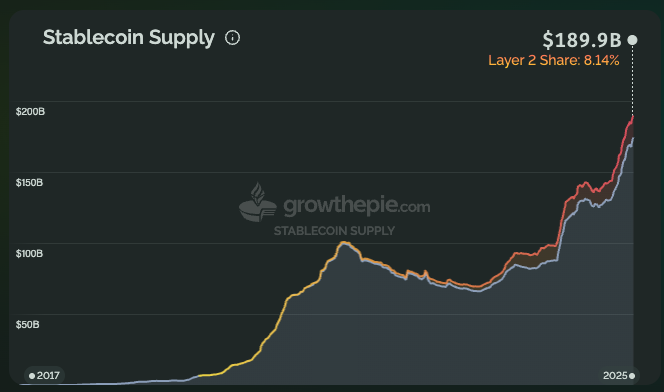
\includegraphics[width=0.9\linewidth]{stablecoins.PNG}
    \caption{\textit{Stablecoins Total Marketcap on Ethereum as of 23OCT2025 - source: \href{https://www.growthepie.com/ethereum-ecosystem/metrics}{Grow the Pie}}}
    \label{fig:enter-label}
\end{figure}

Stablecoins are a far cheaper medium of exchange between participants than traditional rails, faster by three or more orders of magnitude, more secure, and can be private if so desired. They can even be \href{https://x.com/llamapay_io}{streamed by the second.} 

Circle, the American company which built the USDC stablecoin, shocked traditional markets when it peaked at a valuation of over \$70B in the first three weeks of public trading. 

\subsection{Layer 2s}

Ethereum pivoted to the Layer 2 centric roadmap, and in my opinion, this has paid off massively for Ethereum. This was the correct strategic pivot and it will only become more clear as more time passes. 

Robinhood \href{https://robinhood.com/us/en/support/articles/to-catch-a-token-recap/}{announced tokenized equities} in June of 2025 at their keynote \href{https://www.youtube.com/live/FBHmAq5lmZQ?si=MpQUNJN9QSzUSFxr}{"To Catch a Token"} on Ethereum using the Arbitrum layer 2 network and plans to create their own layer 2 on top of Ethereum. It seems they have already tokenized hundreds of assets according to \href{https://dune.com/entropy_advisors/robinhood-stock-tokens}{this dashboard} built by \href{https://x.com/EntropyAdvisors}{Entropy Advisors} that was \href{https://x.com/vladtenev/status/1981472545506525478}{reposted} by CEO Vlad Tenev. 

A layer 2 network brings transaction costs down by an order of magnitude for users by socializing transaction costs across users by aggregating and batching their transactions using advanced cryptography. The most well known and popular layer 2 networks on Ethereum are \href{https://x.com/arbitrum}{Arbitrum}, \href{https://x.com/Optimism}{Optimism}, and Coinbase's \href{https://x.com/base}{Base} network. 

Total Value Locked for Layer 2s on Ethereum is up an impressive amount over the last 4 years:

\begin{figure}[h]
    \centering
    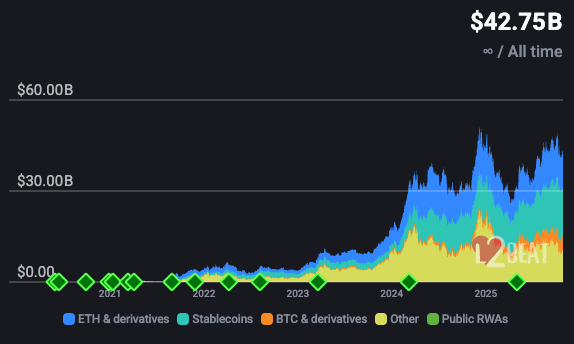
\includegraphics[width=0.8\linewidth]{Layer 2 TVL.png}
    \caption{\textit{Layer 2 Total Value Locked - source: \href{https://l2beat.com/scaling/tvl}{L2Beat}}}
    \label{fig:enter-label}
\end{figure}

\clearpage

\begin{figure}[h]
    \centering
    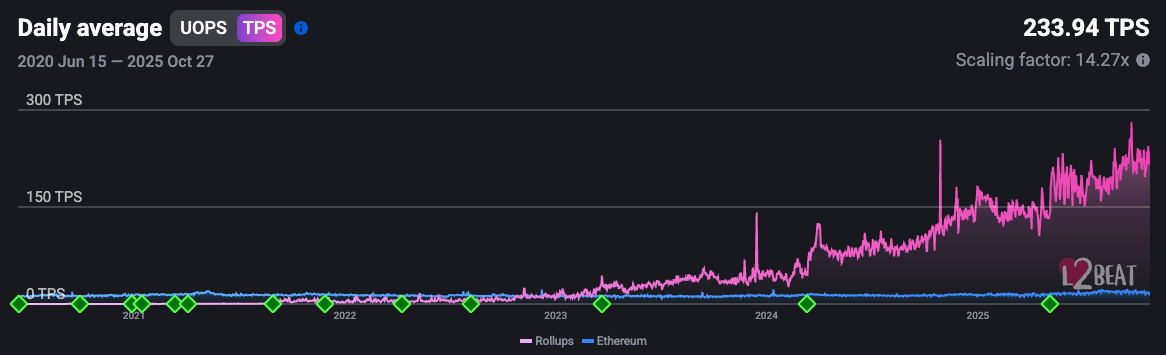
\includegraphics[width=0.9\linewidth]{Layer 2 TPS.PNG}
    \caption{\textit{Layer 2 Total Transactions Per Second - source: \href{https://l2beat.com/scaling/activity}{L2Beat}}}
    \label{fig:enter-label}
\end{figure}

For me, what is even more impressive is the aggregate Transactions Per Second (TPS) of the Ethereum ecosystem as a whole, which has seen an explosion due to new Layer 2s coming online. For reference, I published my first Ethereum paper on 27DEC2021 - when the TPS of the entire Ethereum ecosystem was only $\sim$14 TPS! 

There is still a lot of work to be done - there are ``stages" of development for these layer 2 networks; the best way to think about this is ``how trustworthy a layer 2 is". A deep dive on this concept is in my section on \hyperref[Layer 2s]{Ethereum's Data Layer} later on in this paper.  

\subsection{DeFi}
Over the last four years, we have seen many new applications built on Ethereum; below is a small list of new protocols over the last few years I personally find interesting: 

\begin{itemize}
    \item The Liquid Staking Token sector has come into its own, now worth $\approx$ \$50 Billion as a sector, allowing users to compose on top of their staked ETH for additional yield through utilization in DeFi
    \item \href{https://x.com/Polymarket}{Polymarket} - Prediction market that has gained a large following in the last 12 months, largely due to the 2024 Presidential election
    \item \href{https://x.com/AwakenTax}{Awaken Tax} - the best crypto taxes tool, period. If you use my \href{https://awaken.tax?ref=dm61olox}{referral code}, you'll get 15\% off and I'll get a 15\% revenue share! (This is genuinely a fantastic product, I reached out to the founder to ask for this code, thank you \href{https://x.com/big_duca}{@big\_duca})
    \item \href{https://x.com/SiloFinance}{SILO} - isolated lending markets, think AAVE but with reduced economic risk of an exploit
    \item \href{https://x.com/llamapay_io}{Llamapay} - Llamapay enables payment streaming, imagine getting paid by the second, every second of the day
    \item \href{https://x.com/zkp2p}{ZKP2P} - a way to get paid for offramping your cash via venmo, cashapp, and a few other payment applications
    \item \href{https://x.com/Obol_Collective}{OBOL DVT} - Obol pioneered distributed validator technology (DVT) in Ethereum, allowing stakers to split a validator key between up to 10 participants, increasing validator performance and decentralization. I am part of a cluster with \href{https://x.com/superphiz/status/1730574043508597229}{superphiz}
    \item \href{https://x.com/ensdomains}{Ethereum Name Service} - While not new, it's still cool - imagine having an easy to remember Venmo handle for your ethereum wallet
    \item \href{https://x.com/CoWSwap}{CoW Swap} - The best decentralized exchange (DEX) aggregator on L1 Ethereum for making swaps
    \item \href{https://swap.defillama.com/}{LlamaSwap} - The best DEX aggregator I've found for swaps on Layer 2 networks on Ethereum
    \item \href{https://x.com/safe}{Gnosis Safe} - a fantastic \href{https://www.alchemy.com/docs/multi-sig-contracts}{multisig} wallet for protecting your funds
    \item \href{https://x.com/Rabby_io}{Rabby Wallet} - in my opinion, best wallet for tracking your funds across the Ethereum L1 and L2 ecosystem
    \item \href{https://x.com/0xSplits}{0xSplits} - a great service for automatically splitting payments between participants (or yourself, for tax purposes)
    \item \href{https://x.com/AlchemixFi}{Alchemix} - Self repaying loans. Loans that pay themselves off over time, zero liquidation risk. 
    \item Ethereum ETFs - great for getting exposure to ETH in a tax advantaged retirement account
\end{itemize}

\subsection{Publicly Listed ETH Treasury Companies}

\begin{wrapfigure}{r}{0.45\textwidth}
   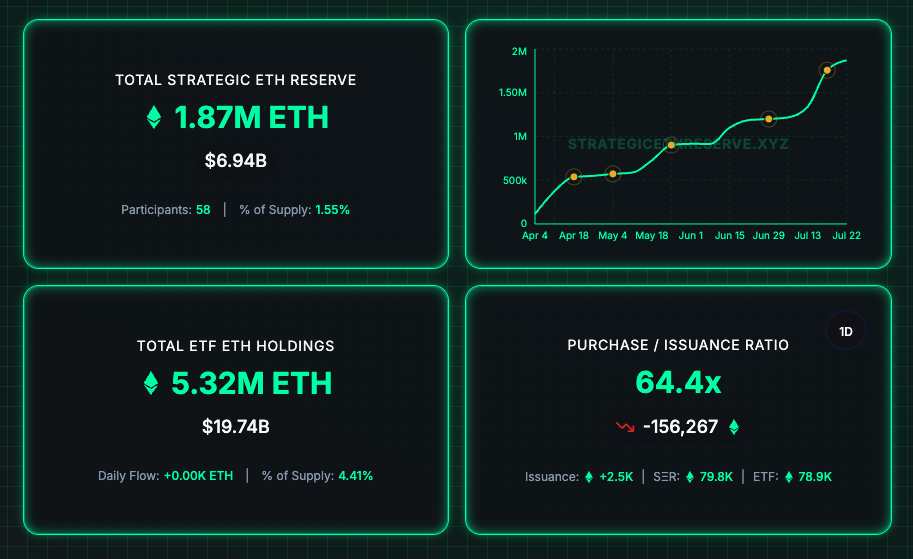
\includegraphics[width=0.45\textwidth]{SER.png}
   \caption*{\textit{The Strategic ETH Reserve - \href{https://www.strategicethreserve.xyz/}{SΞR}}}
\end{wrapfigure}

Starting mid-summer 2025, a handful of publicly listed companies, collectively referred to as Digital Asset Treasury companies (DATs), began the Microstrategy playbook of acquiring Ethereum (rather than Bitcoin, as in Microstrategy's case) and have collectively acquired more than 6 Million Ether. This has solidified Ethereum as a store of value reserve asset, with the added utility that comes along with access to the Ethereum ecosystem, such as yield on staked ETH as well as access to Decentralized Finance protocols, something that Bitcoin cannot offer. These DATs are likely to have an outsized impact on demand for Ether; \href{https://x.com/SharpLinkGaming}{SBET}, with one of the Ethereum co-founders Joe Lubin as its chairman, \href{https://www.sec.gov/Archives/edgar/data/1981535/000164117225020052/form424b5.htm}{intends to acquire} \$5B Ether via at-the-market sales of their stock. Tom Lee from Fundstrat has \href{https://x.com/bitmnr/status/1945857172237393982?s=46&t=e2mii_RCNljiYtI33xapDQ}{a stated goal} of acquiring 5\% (!) of the total supply of Ether - \textit{and is more than half way to his goal!} 

\begin{wrapfigure}{r}{0.4\textwidth}
   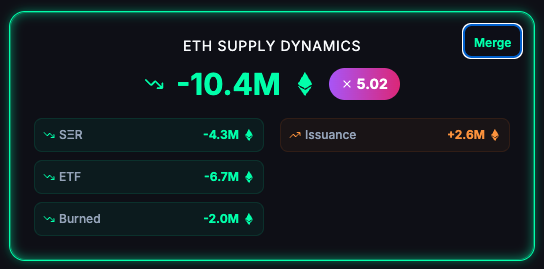
\includegraphics[width=0.4\textwidth]{supply ratio.png}
   \caption*{\textit{5 times as much ETH has been acquired in a DAT, an ETF, or been burnt by tx fees, than has been issued by the network since September of 2022.}}
\end{wrapfigure}

The website \href{https://www.strategicethreserve.xyz/}{Strategic Ethereum Reserve (SΞR)} is a beautiful dashboard for tracking changes in holdings of these companies, as well as other major institutions in the Ethereum community and ETFs that hold Ether. 

One of the coolest aspects about this website is that it tracks daily purchase demand for ETH as a ratio of daily issuance for ETH. On this particular day of writing, approximately 64x as much Ether was purchased as was issued by the network. If this keeps up, it will have a material impact on the price of ETH. 

\subsection{The Merge: Moving from Proof of Work to Proof of Stake}

On September 15th 2022 at block height \href{https://etherscan.io/block/15537394}{15537394}, Ethereum proposed the first Proof of Stake (PoS) block on its network. This was a monumental transition for Ethereum, something that has been a goal for Ethereum since its \href{https://ethereum.org/en/whitepaper/}{whitepaper}, published back in 2014. 

I discuss the benefits of Proof of Stake over Proof of Work in my \href{https://drive.google.com/file/d/1QOn4CBSCqm4lBczFxXCqSBHYueddkAer/view}{paper from three and a half years ago}, but to briefly rehash: 

Ethereum eliminated almost all of its token issuance from Proof of Work (and was even deflationary during a 2 and a half year time period). Ethereum now has close to a 10x multiple of economic security (cost to attack the chain) relative to Bitcoin. Proof of Stake is able to limit the number of times an attacker can successfully attack the network, whereas \href{https://www.youtube.com/watch?v=o8Mg4hzJaFg}{Bitcoin cannot.} Additionally, PoS has benefits around \href{https://dataalways.mirror.xyz/fUBmnyI3Q3KLWzEO7VjQNZzwY_2aTB3AY_7mi99ax2g}{minimizing the Cantillon Effect} relative to Proof of Work systems. 

\begin{figure}[H]
    \centering
    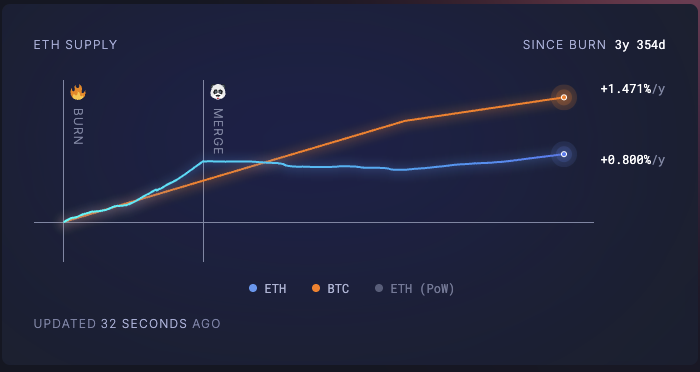
\includegraphics[width=0.75\linewidth]{eth issuance.png}
    \caption{\textit{Since Ethereum moved to PoS, Bitcoin's issuance has far outstripped ETH's issuance over the last four years, image from \href{https://ultrasound.money/}{Ultrasound.money}}}
\end{figure}

If you want to dig deeper on the differences between PoW and PoS, Tim Roughgarden does an excellent deep dive in \href{https://www.youtube.com/watch?v=ZSqxGdsmLHs}{this youtube lecture series} on Proof of Work versus Proof of Stake. 

In April of 2023, Ethereum enabled staking withdrawals, which derisked the full life cycle of staking ETH as validators can be confident they can get their ETH back after a short waiting period. Since then, the amount of ETH staked has \href{https://www.validatorqueue.com/#:~:text=All-,Active\%20Validators,-7d}{close to doubled.}

\section{The Ethereum Improvement Proposal (EIP) Process}

Let's first briefly introduce how the Ethereum community arrives at consensus on which network upgrades to implement (or not implement), before we talk in depth about the roadmap itself. The Ethereum governance process can be messy - no one person or entity is in charge of the process of making decisions - and it is a commonly misunderstood process. This is a brief overview of my understanding of the process, but it does not necessarily happen exactly how I describe below with every upgrade - this is a generalization of the process. 

\begin{wrapfigure}{r}{0.45\textwidth}
   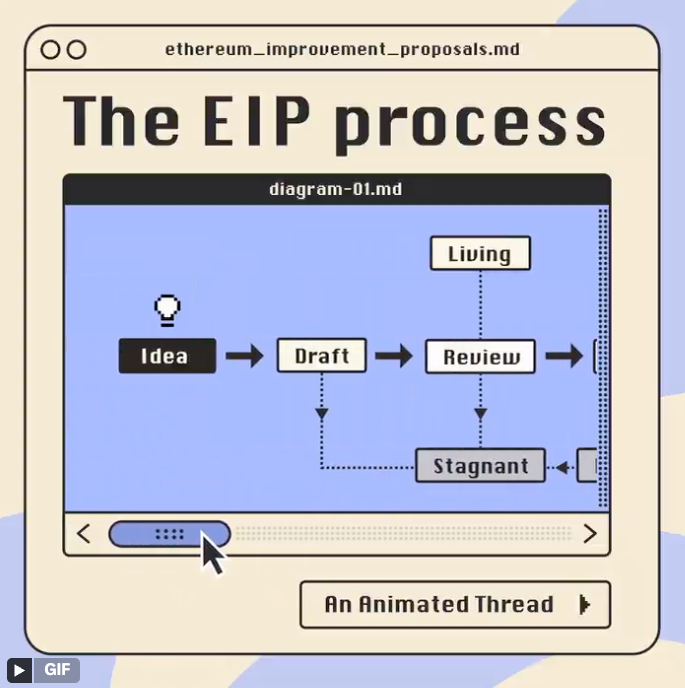
\includegraphics[width=0.45\textwidth]{EIP.png}
   \caption*{\textit{Check out \href{https://x.com/sleety_eth}{Sleety}'s animated \href{https://x.com/tokenmotion_io/status/1851737573300797568}{thread} on the EIP process}}
\end{wrapfigure}

Network upgrades are generally quite involved, so it makes sense to batch groups of EIPs together under a larger network upgrade; these network upgrades have recently been coming out at a cadence of approximately once per year. The naming convention for Ethereum upgrades is a portmanteau of the individual upgrade names for both the Execution Layer and the Consensus Layer. As an example, the currently in progress network upgrade targeted for Q4 2025 is ``Fusaka", a concatenation of ``Fulu" and ``Osaka". Changes to the Execution Layer (EL) have historically been named after cities that have hosted Devcon events, and changes to the Consensus Layer (CL) have historically been named after celestial bodies. 

At a high level, the Ethereum roadmap has many parallel technological upgrades that are all being worked on simultaneously by many different people. The roadmap is split up into focusing on each of Ethereum's three different layers, and the most impactful of these upgrades will be the focus of the rest of this article. 

The community is constantly discussing these research areas online, in \href{https://ethresear.ch/}{forums} and on crypto twitter, and also in person at conferences. Over time, the community coalesces on ideas, and some end up receiving grass roots support from the larger community. Sometimes, more well known community members will signal public support for a particular change to the Ethereum protocol. 

Eventually, a small group of community members who are passionate about bringing that specific change to Ethereum will draft an Ethereum Improvement Proposal, or EIP. This serves as the high level motivation for the upgrade, and doesn't necessarily cover full technical details, as those are usually still in development at this point in the process.  

Anyone can draft and propose an EIP; if an EIP gains enough support from the community, it will end up getting discussed at the bi-weekly ``All Core Developers" call, a public call anyone can watch. There is one for the \href{https://www.youtube.com/watch?v=NQhTiMFDZHQ}{Consensus Layer} - All Core Devs - Consensus (ACDC for short) and one for the \href{https://www.youtube.com/live/1NIvzSliv44?si=0uX_tyXR5qaSijF7}{Execution Layer} (ACDE for short).\footnote{A great example of an EIP being spear headed by a passionate community member was when \href{https://twitter.com/econoar}{Eric Conner} garnered attention and broader community support for \href{https://eips.ethereum.org/EIPS/eip-1559}{EIP-1559}}

At this point, members of the approximately 11 or so different client teams who would actually be responsible for implementing the change to the protocol discuss the EIP as a group. These All Core Devs calls happen regularly on the Ethereum Foundation's \href{https://www.youtube.com/@EthereumProtocol}{youtube channel}, and both \href{https://x.com/TimBeiko}{Tim Beiko} and \href{https://twitter.com/christine_dkim}{Christine Kim} do a fantastic job summarizing these discussions on @X. Christine has also started summarizing these on her podcast \href{https://www.youtube.com/watch?v=ocW16DltZ74}{``The Infinite Jungle"} (although she has since moved on from Galaxy Research, you can find her substack \href{https://christinedkim.substack.com/}{here}).  

It is important to test upcoming network upgrades rigorously, so these large network upgrades will also have multiple devnets and testnets before going live on Ethereum mainnet, where the potential upcoming changes to the network can be tested in as many different failure modes as possible and bugs can be found. 

In June of 2024, Tim Beiko proposed  \href{https://eips.ethereum.org/EIPS/eip-7723}{EIP-7723} to formalize the stages of development for EIPs, and proposed five main stages: 

\begin{itemize}
    \item \textbf{Proposed for Inclusion (PFI)} - someone (can be anyone) has submitted a Pull Request to the meta EIP which tracks the all the proposals for that upcoming hard fork, here is \href{https://eips.ethereum.org/EIPS/eip-7607}{Fusaka}'s Meta EIP
    \item \textbf{Considered for Inclusion (CFI)} - client teams signal their overall support for the EIP so it can move forwards to the next step
    \item \textbf{Scheduled for Inclusion (SFI)} - engineering work is ongoing to include an EIP into the next testnet, and eventually Ethereum mainnet
    \item \textbf{Declined for Inclusion (DFI)} - an EIP has been rejected to be included in this particular network upgrade, but does not mean it will not be included in a future network upgrade. 
    \item \textbf{Included} - the EIPs which ended up going live on Ethereum mainnet are now marked as included. 
\end{itemize}

Tim published a short blog summarizing EIP-7723 discussing these proposed changes to the process \href{https://tim.mirror.xyz/CuRtFjkujKBqVsdvCGvthiPIYaZyzNc5sWIaExw2UpE}{here.} Tim has said his aim with this EIP was to ``facilitate the process, without slowing it down bureaucratically." 

\section{What is next for Ethereum? The Technical Roadmap}

\subsection[\protect\textbf{\small The Blockchain Trilemma}]{The Blockchain Trilemma}

Around Ethereum's 10th Birthday, Justin Drake published a blog post titled \href{https://blog.ethereum.org/2025/07/31/lean-ethereum}{``Lean Ethereum"} where he lays out Ethereum's goal and how to get there.  

\begin{itemize}
    \item \textbf{Ethereum' Goal:} Become the neutral, censorship resistant \textit{``bedrock of the internet of value, securing hundreds of trillions over decades, even centuries."}
    \item \textbf{How to Get There:} Upgrades to Ethereum's three layers:
    \begin{itemize}
        \item \textbf{Consensus Layer} - the layer for establishing Ethereum's economic finality
        \item \textbf{Execution Layer} - the layer responsible for executing users' transactions
        \item \textbf{Data Layer} - the layer responsible for being a public bulletin board for rollups posting their post-execution data to Ethereum
    \end{itemize}
\end{itemize}

 Justin also \href{https://www.youtube.com/watch?v=8mJDt8TGebc}{gave a talk} at the \href{https://www.youtube.com/watch?v=zeNVsuO_fts&list=PLmkdAgtxf3aidisFxgAfbe7AuMmruh4qE}{Bankless summit} discussing his view of the Roadmap at a high level over the next 5 year time horizon. He discussed how each technical upgrade to Ethereum either improves \textbf{execution throughput}, increases \textbf{data availability}, or hardens and democratizes the \textbf{consensus} layer. Justin briefly discussed each of these layers in his Lean Ethereum blog post, and each upgrade that I dive into in this paper will be bucketed into one of these three layers.
Before we move on to the rest of the article - a quick refresher on the blockchain trilemma, with an excerpt from my article from three years ago: \\

\begin{aside}
\begin{wrapfigure}{r}{0.37\textwidth}
   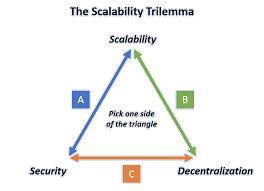
\includegraphics[width=0.45\textwidth]{blockchain_trilemma2.png}
   \caption*{\textit{The Blockchain Trilemma}}
\end{wrapfigure}


\emph{``Historically, blockchains have suffered from the blockchain trilemma - the trade off between security, decentralization, and scalability. Blockchains have had to choose between optimizing for two of these three properties. A brief definition of these three terms:}


\emph{
\begin{itemize}
    \item \textbf{Decentralization} refers to a blockchain's ability to both be credibly neutral and censorship resistant. The less prohibitive it is to become a node operator and validate the chain, the more validators there will be, and the more decentralized the chain will be. 
    \item \textbf{Security} can refer to the cost to successfully attack a network. The more costly it is to attack a network and extract monetary value, the more secure that network is. 
    \item \textbf{Scalability} refers to the number of transactions per second a chain is capable of. If a blockchain can increase its TPS, transaction fees can be set lower, making it more accessible to a higher number of users." 
\end{itemize}}

\end{aside}

The Ethereum road map should be thought about in the context of the blockchain trilemma. Ethereum's technical roadmap is about finding the right tradeoffs in a complicated tradeoff space. The essence of engineering is navigating tradeoff spaces. The blockchain trilemma is the most important tradeoff space all cryptocurrencies must navigate. 

Ethereum's most important properties are security and decentralization, so Ethereum chooses to optimize for these two properties. Ethereum's properties of reliability (\href{https://ethereumuptime.org/}{100\% uptime} since inception), credible neutrality, and censorship resistance, are downstream of its decentralization and security. Every upgrade discussed below is an effort to improve Ethereum's scalability (transaction per second) or its user experience (UX), \textit{without compromising on its values of security and decentralization}. Improving Ethereum's overall TPS will be crucial if it is to become the global center of financial gravity. \href{https://forkcast.org/upgrade/fusaka}{Forkcast,} a community resource for quick references to coming upgrades to the network that are in progress, does a fantastic job highlighting how each individual potential change to the network contributes to either increased scalability to the network or improving UX. 

\subsection[\protect\textbf{\small Ethereum's Consensus Layer}]{Ethereum's Consensus layer}

What is Ethereum's Consensus Layer? What is it responsible for?

The Internet's participants consist of people and entities that do not share interests and do not trust each other. On top of this, the internet is built on unreliable infrastructure and every participant will have a slightly different view of exactly what is happening on the chain. So how do we decide on exactly one history of the blockchain such that no participant needs to trust any other participant, using unreliable internet connections where not every node will always be online? This is the challenge of establishing consensus. 

Proof of Work systems establish consensus by relying on cryptographic randomness and economic incentives. The next block proposer is chosen by whichever miner finds the output of a hash function with a certain number of zeros in front of it. Bitcoin miners then continue mining on the chain with the most amount of total work, to minimize the odds that their work done is wasted. These two mechanisms establish \textit{probabilistic finality}. The difficulty of finding the correct output and becoming the next bitcoin block proposer adjusts dynamically to target an average block time of approximately ten minutes; this is called the ``difficulty adjustment". Because \href{https://www.youtube.com/watch?v=orIgy2MjqrA&t=214s}{no one can predict} the outcome of the hash function without actually just doing the work, the odds that someone is able to revert block history \href{https://www.youtube.com/watch?v=S9JGmA5_unY}{is incredibly small}, (although still non-zero!).\footnote{If the individual miners of the largest bitcoin mining pool, Foundry USA, (~30\% of total hash rate) decided to coordinate to revert the most recent hour's worth of bitcoin block history, it would have $\sim$1\% chance of being successful at this. } 

In contrast, Proof of Stake systems offer \textit{deterministic finality}, unless a significant sum of money is destroyed to change block history that has been finalized. This is because Ethereum Proof of Stake sibyl resistance \textbf{does not} rely on cryptographic randomness to select the next block proposer, and instead relies on \href{https://eth2book.info/capella/part2/building_blocks/randomness/}{endogenous protocol pseudo-randomness} proportional to stake. Proof of Stake systems must provide a guarantee that in order for an attacker to be successful, it must be verifiable that a successful attack would cost a significant sum of money. This concept is called \textbf{Economic Finality}, and in order for finalized block history to change, an obscenely large amount of capital must be provably destroyed. In Ethereum's case, an attacker gets \textit{slashed} if conflicting statements are made about chain history. With 35.7 Million ETH staked, 1/3rd of all staked Ether is today worth $\approx$\$48 Billion, or approximately three (!) nuclear powered aircraft carriers worth of value, such that it is exceedingly unlikely to be a profitable endeavor. 

In blockchains, no one participant's view of the chain can be accepted as truth, so Ethereum uses its Consensus Layer, which is composed of a few different mechanisms that work together, to establish both the canonical history of the chain and for selecting the next block that will be appended to the chain. 

One of these mechanisms is ``forward looking", in the sense that it is responsible for choosing the next canonical block in the chain. The other one is ``backwards looking", in the sense that it cements groups of 32 blocks, also known as epochs, into Ethereum's history (unless an extremely large amount of capital is destroyed) through the finalization process:
\label{Gasper}

\begin{itemize}
    \item \href{https://eth2book.info/capella/part2/consensus/lmd_ghost/}{LMD GHOST:}  A combination of two acronyms, ``Last Message Driven" ``Greedy Heaviest Observed Sub-Tree" is the forward looking mechanism of the two. LMD GHOST picks the next block which will be appended to the front of the chain; the block that gets chosen is the block (must be a valid one) that has the most amount of economic weight voted in favor of it and is referred to as the ``Head" of the chain. Validators submit their local view of the head of the chain; these votes are called attestations. LMD GHOST aggregates validators' view of the head of the chain, weighted by stake; the block with the most economic weight from validators' submitted attestations establishes the head of the chain. 
    \item \href{https://eth2book.info/capella/part2/consensus/casper_ffg/}{Casper FFG:} The Casper Friendly Finality Gadget is the backward looking mechanism of the two and uses a process called \textit{finalization}. Finalizing blocks is a sequential two step process; first justification, then finalization. Blocks get finalized in groups of 32 blocks; each group of 32 blocks is called an epoch. 

    \begin{itemize}
        \item \textbf{Justification:} when an individual validator attests to a group of 32 blocks, or epoch, that validator is making a commitment to never revert the chain history prior to that epoch and broadcasts this to the network. Once $>$ 2/3rds of the network have committed to never reverting that epoch, it is considered justified. But because every validator's view of the network is unique to that validator, this is not enough to finalize a block - you have to be confident that $>$ 2/3rds of the network have also justified the block and \textit{then you have to tell the rest of the network what you heard was justified.}
        \item \textbf{Finalization:} For that block to be finalized, you must communicate to the network what you heard was justified by the network in the previous step. Only after you have heard what the rest of the network heard in step 1 can you be confident that $>$2/3rds of validators have committed to and finalized that particular epoch.
    \end{itemize}
\end{itemize} 
\label{Finality}

\begin{figure}[H]
    \centering
    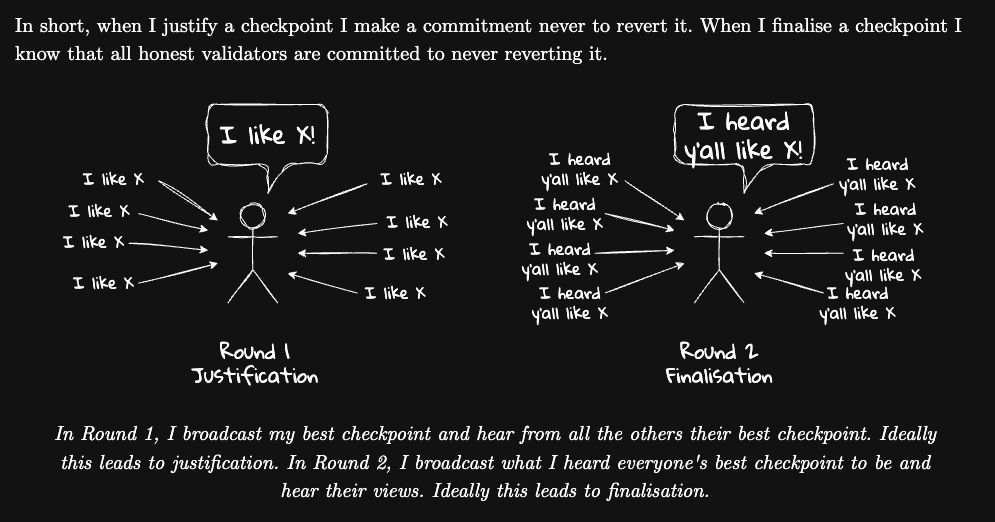
\includegraphics[width=0.9\linewidth]{justification finalization.png}
    \caption{\textit{Above is a fantastic visualization of justification and finalization from Ben Edington's \href{https://eth2book.info/capella/part2/consensus/casper_ffg/}{blog}}}
\end{figure}

The combination of the ``forward looking" LMD GHOST mechanism, responsible for selecting the next canonical block, and the ``backward looking" Casper FFG mechanism, responsible for finalizing block history, together make up Ethereum's Proof of Stake consensus. The combination of these two mechanisms is called \href{https://ethereum.org/developers/docs/consensus-mechanisms/pos/gasper/}{Gasper} and it provides both the properties of \textit{accountable safety}, ensuring that conflicting epochs cannot be finalized without verifiable proof of misbehavior (which results in slashing, or the destruction of, some of the attacker's staked capital), and the second property of \textit{liveness}, meaning that it is always possible for the chain to continue finalizing new blocks. Both properties are defined on page 7 of \href{https://arxiv.org/pdf/2003.03052}{this paper} by the Ethereum Foundation in coordination with \href{https://x.com/SJSU}{SJSU} and \href{https://www.vinai.io/}{VinAI.} 

We now have three ``stages" in the life cycle of an epoch:

\begin{itemize}
    \item \textit{Prejustification: \small(I made this term up to communicate the idea but it's not a formal term)} \normalsize A block has been selected by the LMD GHOST mechanism as the head of the chain, it has been \textit{provisionally} accepted by the chain
    \item \textit{Justification:} $>$2/3rds of the validator set have now committed to never reverting this epoch
    \item \textit{Finalization:} $>$2/3rds of the network is now \textit{aware} that $>$2/3rds of the network has committed to never reverting that epoch and it is now considered final
\end{itemize}
\clearpage
\begin{aside}
    An Informal Mathematical Proof of Economic Finality \textit{(Warning: A small bit of math)}\\
    \\
    In the case where two conflicting blocks are attested to by the network, at least 1/3rd of the validators \textit{must have voted for both conflicting blocks}, and will get slashed. What follows is a proof of this statement. The validators making conflicting attestations would then get slashed, meaning they would lose some fraction their staking deposit, and get booted from the validator set for their misbehavior. This is why their deposit is considered ``at stake". 

    By definition, in order for a block to be considered final, it must have $>$2/3rds of validator stake weight to have voted for that block. Let's define $V_{total}$ as the total validator set and $V_A$ as a subset greater than or equal to 2/3rds of the total validator set $V_{total}$. $V_A$ votes for block $A$. $V_B$ is another subset greater than or equal to 2/3rds of $V_{total}$, but $V_B$ votes for block $B$, which conflicts with block $A$. 

    To find the fraction of validators that voted for both conflicting blocks $A$ and $B$, we can add $V_A$ and $V_B$ and subtract $V_{total}$, then solve for the overlapping fraction of total validators that voted for both conflicting blocks, let's call this fraction $\frac{some}{fraction}$ (this is what we will solve for.) 

\begin{align}
    (V_A+V_B)- V_{total} \quad > \quad \frac{some}{fraction}V_{total}
\end{align}

Since we know both $V_A$ and $V_B$ must both be greater than 2/3rds of $V_{total}$ by definition, let's replace $V_A$ and $V_B$ with the inequality $>2/3V_{total}$

\begin{align}
    (>\frac{2}{3}V_{total})+(>\frac{2}{3}V_{total}) - V_{total} \quad > \quad \frac{some}{fraction}V_{total} 
\end{align}

Combining terms and simplifying, we now know that $\frac{some}{fraction}$ must be greater than or equal to $>1/3rd$ of total validators, meaning at least 1/3rd of the validator set gets slashed. 

\begin{align}
    (>\frac{4}{3}V_{total}) - V_{total} \quad > \quad \frac{1}{3}V_{total} 
\end{align} 

This slashing condition now holds validators at economic risk if they submit conflicting votes that violate the consensus rules of the protocol, resulting in a significant amount of capital being destroyed. If you want to learn more specifics about the slashing mechanism, you can read 
\href{https://x.com/benjaminion_xyz}{Ben Edgington}'s blog called the ETH2 book 
\href{https://eth2book.info/capella/part2/incentives/slashing/}{here.} 
    
\end{aside}

For Ethereum to achieve economic finality today, it takes two epochs to have passed with greater than 66\% of stake having attested to the validity of those Epochs. Because each Epoch has 32 individual 12 second blocks, Ethereum today achieves economic finality after about 12.8 minutes. This is deterministic economic finality - for state history older than 12.8 minutes to be changed, a large amount of staked Ether must be destroyed, approximately \$48 Billion in ETH as of writing!

Ethereum today has about $\approx$ 35.7 Million \href{https://beaconcha.in/}{ETH staked}, which represents just over \$145 Billion in capital at stake, or \$48 Billion in economic security. 
\clearpage
\subsubsection{Improving Ethereum's Consensus Layer}

There are three main parts to improving the Consensus Layer, their goals are to: 


\begin{itemize}
    \item improve the rapidity of achieving \textbf{economic finality} by implementing \textbf{Single Slot Finality}
    \item provide better inclusion guarantees using both shorter block times and also \textbf{preconfirmations}
    \item make Ethereum less susceptible to \href{https://en.wikipedia.org/wiki/Denial-of-service_attack}{Distributed Denial of Service (DDOS)} attacks by implementing \textbf{Single Secret Leader Election}
\end{itemize}

\subsubsubsection{Single Slot (Economic) Finality}
\label{Single Slot Finality}

A block is supposed to be proposed to the network every 12 seconds, but because blocks can be missed if a block proposer is offline for example, this 12 second window for a block proposal is referred to as a ``slot". The goal is to achieve economic finality every slot. This is \textbf{Single Slot Finality} (SSF). Achieving economic finality every 12 second slot would mean achieving finality approximately 20x faster than today. 

Why do we care about Single Slot Finality? If Ethereum wants to be the nexus of financial settlement for the world, it will need to be custodying trillions of dollars worth of value. For organizations who manage this wealth to be comfortable entrusting Ethereum to custody those funds, achieving a very strong economic guarantee that block history will not change after two 12 second slots (24 seconds in total), in contrast to the current $\sim$ 12.8 minute guarantee today, will be a critical component to attracting that amount of wealth to settle on Ethereum in the first place. 

Single Slot Finality is really a mis-nomer, as finality would take more than just one slot. The LMD-GHOST and Casper FFG mechanisms would still apply, except now every block gets a Casper FFG vote, instead of just the first block in each epoch (every 32 blocks). Just as before, there would be three stages: \textit{prejustification}, where a block has been provisionally accepted by the chain as the head block by the LMD-GHOST mechanism, \textit{Justification}, where $>$2/3rds of the validator set have committed to never reverting this block, and \textit{Finalization}, where $>$2/3rds of the validator are assured that $>$2/3rds of the rest of the validator set have committed to that block to canonical chain history. 

So, why does Ethereum's finalization process happen in \textit{groups of 32 blocks at a time,} i.e. at the resolution of 32 blocks, today? Why not execute the same two step process of justification and finalization, just at the resolution of single blocks as described above?

The underlying constraint here is \href{https://notes.ethereum.org/@vbuterin/single_slot_finality#What-are-the-issues-with-developing-an-optimal-aggregation-strategy}{\textit{signature aggregation}} - that it is difficult to aggregate so many signatures in a short enough time frame. Attestations are essentially public commitments from validators to \hyperref[Finality]{never revert block history}. The contents\footnote{An attestation contains a Casper FFG vote to establish finality and an LMD-GHOST vote to select the head of the chain, more \hyperref[Gasper]{here.} } of these attestations are signed, which proves which validator submitted which attestation. 

Today, there are about 1 Million validators who must submit attestations. Verifying 1 Million signatures from each individual validator is not practical inside of a 12 second slot, so to make this more practical, validators submit an attestation only once every 32 blocks, which averages out to $\approx$ 32,000 signatures per 12 second slot. Verifying all 32,000 signatures inside of 12 seconds is still a challenge however, so an additional measure is taken. The signatures are \href{https://eth2book.info/capella/part2/building_blocks/signatures/#aggregation}{aggregated} prior to verification; for signature aggregation, Ethereum relies on two properties of elliptic curve cryptography,  \textit{elliptic curve addition} (ECADD) for signature aggregation and \href{https://en.wikipedia.org/wiki/BLS_digital_signature}{\textit{BLS pairings}} for signature verification. 

\begin{wrapfigure}{r}{0.6\textwidth}
   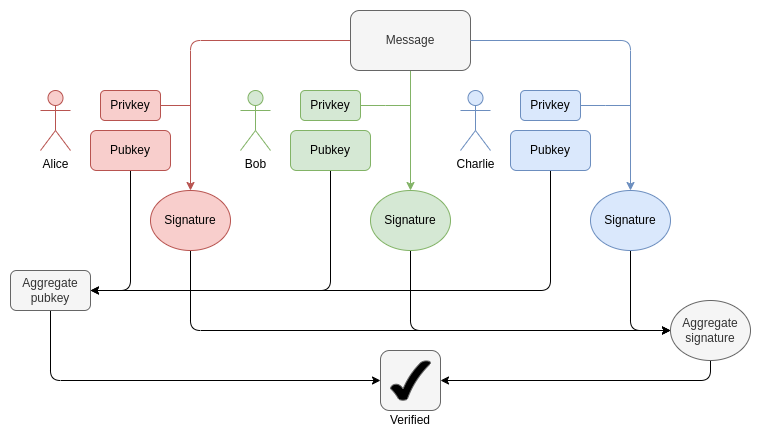
\includegraphics[width=0.6\textwidth]{signature aggregation.png}
   \caption*{\textit{signature aggregation, from \href{https://vitalik.eth.limo/general/2024/10/23/futures4.html\#:\~:text=How\%20BLS\%20aggregation\%20works.}{Vitalik's blog}}}
\end{wrapfigure}

Aggregating signatures is a form of consolidation, where adding signatures results in a \textit{combined} signature that maintains the properties of an individual signature. The aggregated signature can then itself be verified using BLS pairings; if the result is valid, the entire group of signatures that were added together are also all valid. Signature aggregation reduces the work load of verifying 32,000 individual signatures down to verifying only 128 groups of $\approx$ 250 signatures per slot, which is a significant savings. This is not a computationally intensive operation, but the challenge becomes aggregating the signatures fast enough if we are to move towards achieving finality at the slot resolution (every 12 seconds) rather than at the epoch resolution (32 slots, 6.4 minutes).

Moving towards achieving finality at the resolution of single blocks would then require aggregating signatures from the entire validator set of one million validators every 12 seconds, which cannot be done quickly enough using ECADD and BLS verification operations without compromising on Ethereum's goal of keeping validator hardware requirements low. 

To solve this challenge, there are two main competing approaches to achieving Single Slot Finality: 

\begin{itemize}
    \item \textbf{Aggregate signatures more quickly:} Improve the signature aggregation scheme by using recursive SNARKs such that we can aggregate $>$ 1M signatures every twelve seconds (easier said than done)
    \item \textbf{Reduce the number of signatures} that need to be aggregated every slot via an \textit{orbit mechanism}
\end{itemize}

\subparagraph{We can aggregate signatures faster} by deprecating the SHA-256 hash function in favor of a much faster, zk-proof friendly hash function called Poseidon. Then, we generate zero knowledge proofs that the signatures were aggregated correctly using the concept of \href{https://hackmd.io/dR4V2ZJmSfC4VNFob_2lRA#52-SNARK-2-Hash-based-recusive-SNARK-to-replace-BLS-Sig-Aggregation}{\textit{recursive SNARKs}}. A SNARK is a Succinct Non-interactive ARgument of Knowledge, a mathematical proof that can be used to prove that a mathematical operation was performed correctly.  SNARKs can be recursively stacked, meaning SNARKs can be iteratively generated to prove the correctness of other SNARKs, which compounds their efficiency. The benefit here being that, a validator would only be responsible for verifying the correctness of one proof that represents the entire validator set of 1M validators, a very computationally simple task. 

To move towards a zk-proof centric consensus layer, we must prove the state transition function of the consensus chain, which primarily involves constructing proofs of all three main functions of the beacon chain: signature aggregation using ECADD operations, verifying the aggregated signatures using pairings, and verifying the state itself. This is likely a few years away, but is in progress. 

\subparagraph{Or, we can just reduce the number of signatures required per slot} by using an Orbit mechanism, as described by Francesco in this \href{https://youtu.be/6VEEAemYaeI?si=4Jm8hafnxuHfrFzt}{talk}.  

There are two requirements to implement this approach: 

\begin{itemize}
    \item \textit{validator consolidation:} this involves increasing the maximum size of one validator from 32 ETH to 2048 ETH, allowing node operators to combine up to 64 validators into one. This \href{https://consensys.io/blog/ethereum-pectra-upgrade#:~:text=EIP\%2D7251\%3A\%20Increase\%20the\%20MAX_EFFECTIVE_BALANCE}{already happened} with the Pectra upgrade in May of 2025, and has some great benefits, even if we don't end up implementing an orbit mechanism after all. 
    \item \textit{Establishing attester committees:} attester committees would be responsible for attesting to block validity and involve randomly selecting validators proportional to their stake size as a fraction of the maximum validator size of 2048 ETH per validator. The membership of each committee would rotate, hence the ``orbit" naming of this mechanism. 
\end{itemize}

Validator consolidation, proposed in \href{https://eips.ethereum.org/EIPS/eip-7251}{EIP-7251}, allows node operators, potentially running many validators on one machine already, to now consolidate as many as 64 validators with 32 ETH each, down to one validator securing 2048 ETH.  This aims to reduce the total number of validators on the network while still maintaining the same number of unique validator entities, which would ultimately reduce the amount of validator signatures that need to be aggregated each epoch without harming decentralization. This has the added benefit of allowing smaller node operators to compound their stake, whereas before, they would have to wait to add an additional validator at increments of 32 ETH. For some metrics on validator consolidations: \href{https://pectrified.com/mainnet}{pectrified.com}

The attester committees would then be responsible for attesting to each block. The committee's membership rotates, with the probability a validator is selected to participate in a particular committee proportional to the size of its stake as a fraction of the maximum validator size. Validators with 2048 ETH would be a part of every committee, while validators with 32 ETH would only participate every 64 blocks on average (half as often as today). The chances of being selected for a committee increases linearly with validator size until it hits 100\% at 2048 ETH. Each validator would still earn the same rewards on a per ETH secured basis.  This would result in committee sizes of less than 30k validators per slot, making signature aggregation from validators' attestations practical. 

In this \href{https://ethresear.ch/t/orbit-ssf-solo-staking-friendly-validator-set-management-for-ssf/19928}{post} on the ethresearch forum, \href{https://x.com/fradamt}{Francesco} explores a few different approaches to Orbit SSF, and at the end discusses economic incentives to promote Validator consolidation of large validators, since the network cannot force validators to consolidate their stake. 

The end result is that economic finality is achieved far faster with an Orbit mechanism than it is in today's finality mechanism which takes 64 slots (12.8 minutes). 

One of the tradeoffs that the Orbit mechanism's approach to SSF makes, as Vitalik points out in his \href{https://vitalik.eth.limo/general/2024/10/14/futures1.html#:~:text=but%20are%20okay%20with%20the%20cost%20of%20attack%20being%20perhaps%2010x%20less%20than%20today}{blog}, is that Ethereum's economic security would be \textit{limited by the stake size of each committee}, effectively reducing it's overall economic security. 

\subsubsubsection{Single Secret Leader Election}
\label{Single Secret Leader Election}

One of the core responsibilities of a blockchain is being un-censorable. By extension, this means always being available. Ethereum has had \href{https://ethereumuptime.org/}{100\% uptime.} This is largely because of Ethereum's multi-client architecture. 

One risk to Ethereum's availability is the fact that the next two epochs' block proposers (64 blocks in total), although chosen \href{https://eth2book.info/capella/part2/building_blocks/randomness/}{in a pseudo-random fashion}, are made public to the network. An attacker could theoretically Denial-of-Service (DoS) attack those proposers to bring the network down. 

And this kind of attack is not unprecedented. Hudson Jameson tells his \href{https://www.youtube.com/watch?v=hYPCtij_h4o}{first hand account} of being involved in the disaster response while he was at the Ethereum Foundation during the 2016 Shanghai Attacks. These were a form of attempted DoS attacks, although they were not targeted at specific validators because this was in 2016, four years before Ethereum's PoS Beacon chain went live. 

The concept to mitigate this kind of attack is rather simple, but there are complexities that make implementation much more difficult in practice. The idea is to keep the identity of the next proposer private as long as is possible, and ideally, up until the block is actually proposed to the network by the proposer. 

The process of selecting the next proposer is called \href{https://a16zcrypto.com/posts/article/leader-election-from-randomness-beacons-and-other-strategies/}{``Leader Election"}. Making leader election ``secret" involves only the selected proposer knowing that they will be proposing a block at some point in the near future, and each block will need to be proposed by one proposer (unless we move towards a multi-proposer architecture). Putting it together, we get Single Secret Leader Election, SSLE. What makes SSLE difficult is the combination of the leader election being \textit{both} secret \textit{and} single (only selecting one proposer.) Tim Roughgarden explains some of the intricacies of this beginning in \href{https://www.youtube.com/watch?v=au-pyenGexg}{episode 12.8} in his \href{https://www.youtube.com/watch?v=ZSqxGdsmLHs&list=PLEGCF-WLh2RLOHv_xUGLqRts_9JxrckiA&index=62}{series} on Proof of Stake sybil resistant protocols.  

Personally, I think there's a decent chance we won't see an implementation of SSLE in Ethereum until after zero-knowledge proofs become core to the protocol. 
\clearpage
\subsubsubsection{Preconfirmations}
\label{Preconfirmations}

One of the user experience challenges in Ethereum today is the fact that users are faced with 12 second block times; this delay can cause uncertainty around how exactly a submitted transaction gets executed onchain. 

\begin{wrapfigure}{r}{0.5\textwidth}
   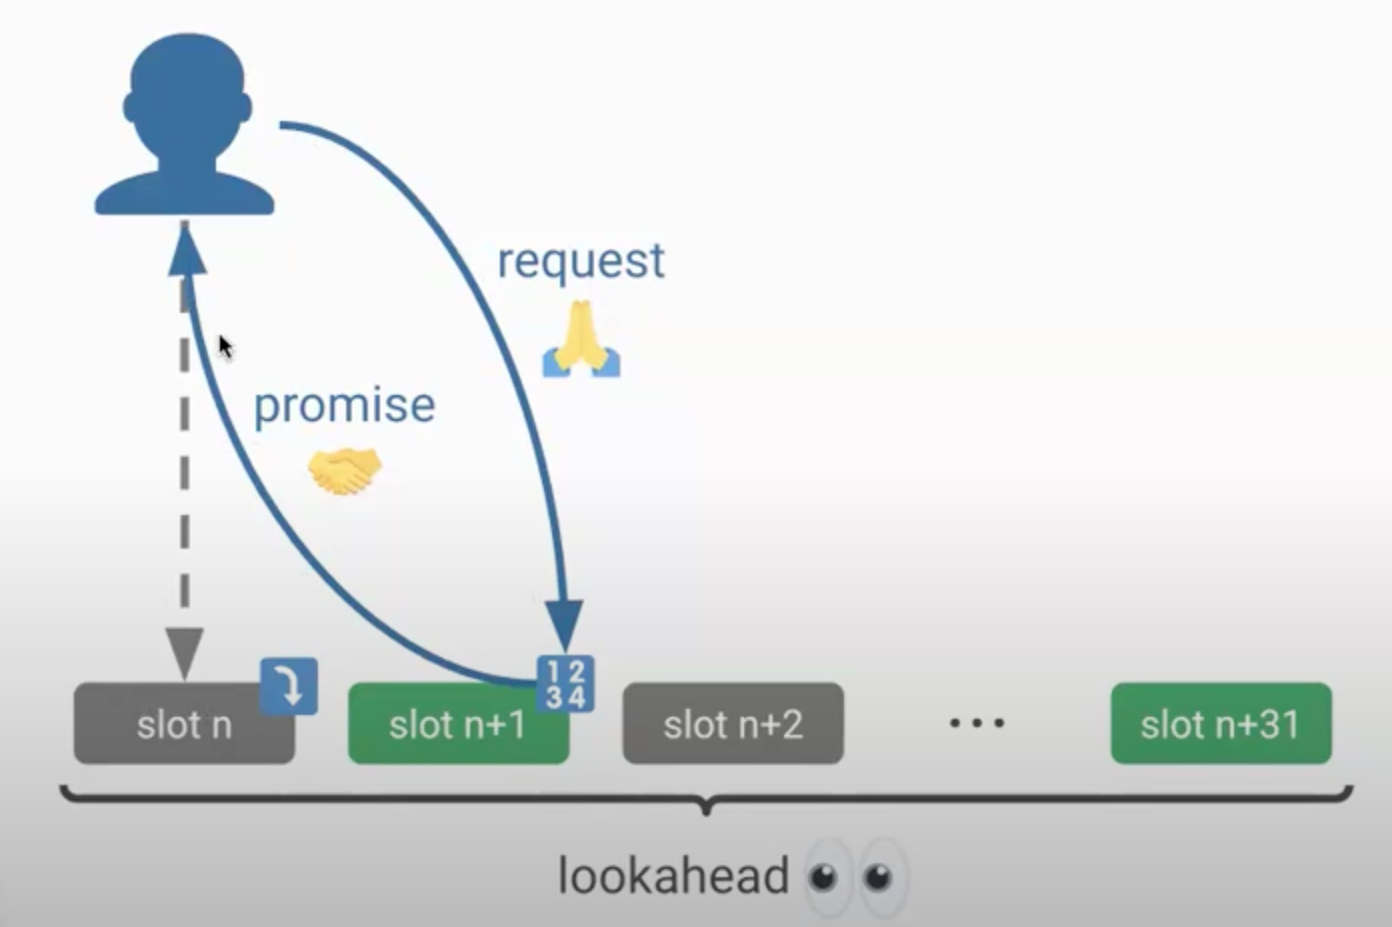
\includegraphics[width=0.5\textwidth]{incl and seq.png}
   \caption*{\textit{From the \href{https://www.youtube.com/watch?v=2IK136vz-PM}{Sequencing and Preconfirmations call \#1}}}
\end{wrapfigure}

To address this, Justin Drake \href{https://ethresear.ch/t/based-preconfirmations/17353}{has proposed} the concept of a preconfirmation, which he discusses in detail in this \href{https://www.youtube.com/watch?v=2IK136vz-PM}{talk}. Preconfirmations involve a proposer providing a promise of transaction inclusion in return for a tip from the user and at the risk of slashed collateral if the proposer reneges on their promise. Preconfirmations would improve Ethereum's UX by providing increased certainty for users that their transaction will be included onchain in a time frame that is more than an order of magnitude faster than the L1 block time of 12 seconds. 

%\begin{figure}[H]
%    \centering
%    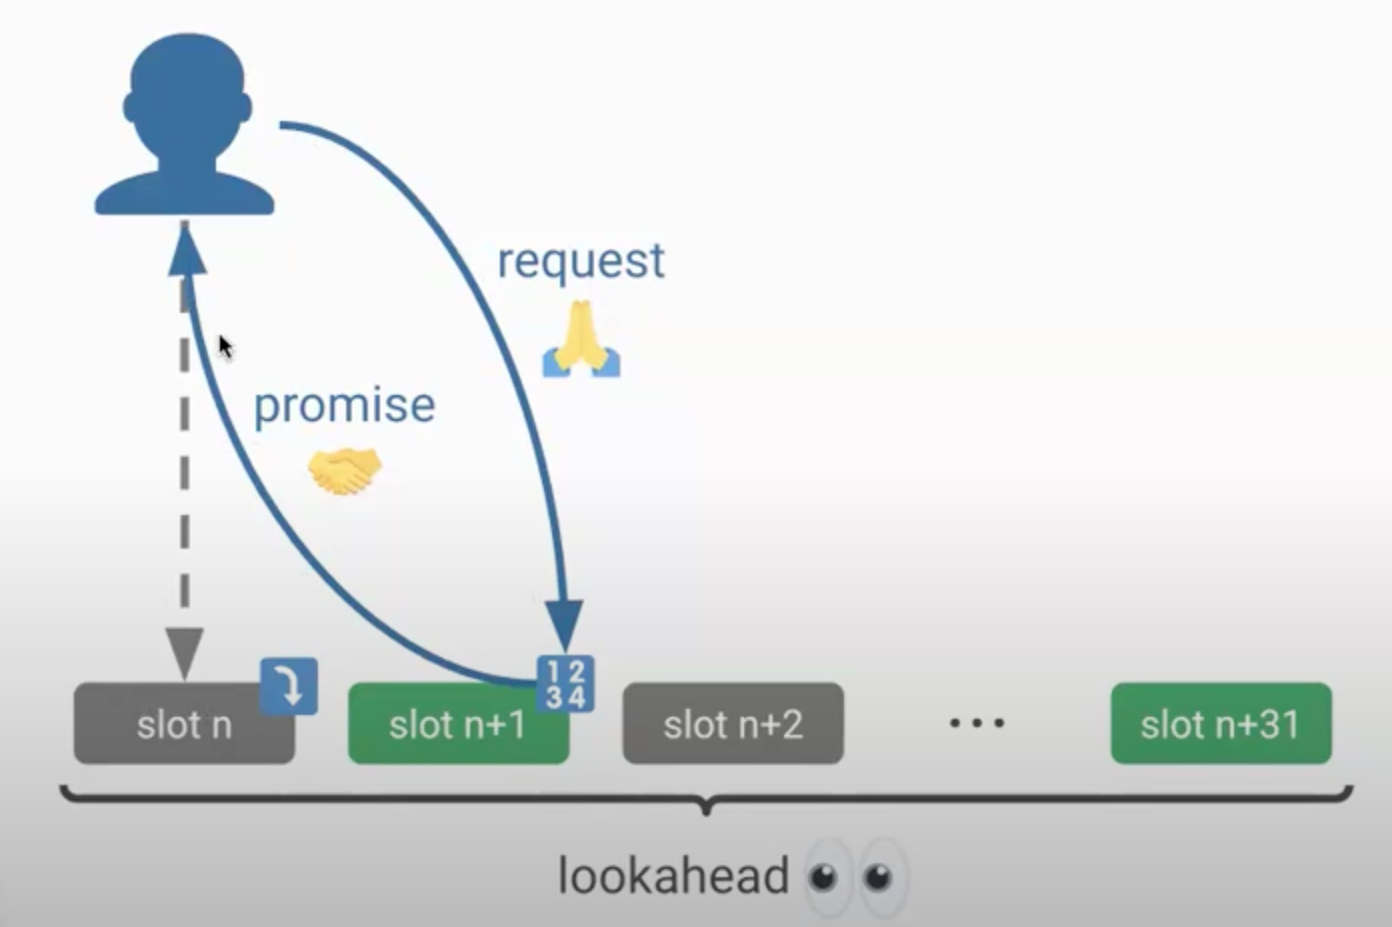
\includegraphics[width=0.7\linewidth]{incl and seq.png}
%    \caption{\textit{From the \href{https://www.youtube.com/watch?v=2IK136vz-PM}{Sequencing and Preconfirmations call \#1}}}
%\end{figure}

In order to have the ability to promise inclusion for a submitted transaction, an L1 proposer must have the right to sequence transactions. Sequencing rights involve the ability to place submitted transactions in any order, and it is usually auctioned off to a block builder that can order transactions in the most profitable way, referred to as maximizing extractable value \hyperref[MEV]{(MEV)}. Because an L1 proposer enjoys monopoly power over sequencing by definition, that proposer can accept requests for the preconfirmation of a transaction and then utilize their monopoly power of transaction sequencing to ensure that transaction gets included in a timely manner. 

\begin{wrapfigure}{r}{0.5\textwidth}
   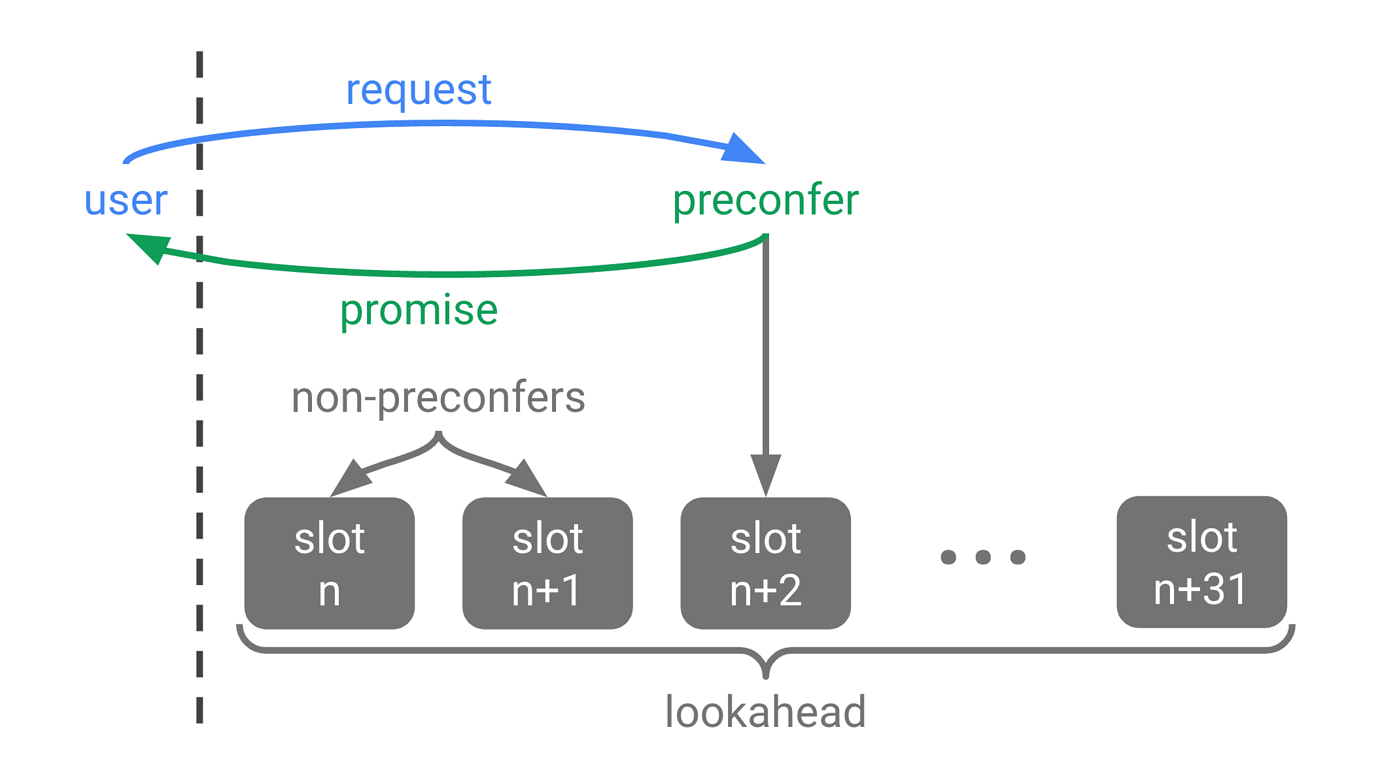
\includegraphics[width=0.5\textwidth]{preconfer.png}
   \caption*{\textit{Being an L1 preconfer for validators would be optional}}
\end{wrapfigure}

Preconfirmations could reduce the perceived block time on Ethereum L1 to just hundreds of milliseconds, a vast UX improvement over the 12 second block time users experience today. 

L1 proposers that opt in to provide preconfirmations are referred to as preconfers and would voluntarily run a sidecar software (in the same way that MEV-boost is a sidecar that \href{https://dune.com/dataalways/staking}{most of the validator set runs} voluntarily) that allows users to submit requests for transaction preconfirmations. The incentive for a proposer to do this would be additional revenue from the tips users submit when requesting a preconfirmation. 

Users submitting preconfirmation requests can be reasonably sure their transactions will be included because of two slashing conditions that \href{https://ethresear.ch/t/based-preconfirmations/17353}{Justin proposes} that would result in the preconfer losing some amount of collateral. Those are: 

\begin{itemize}
    \item \textbf{Liveness fault:} occurs when a slot is missed and the user's transaction is not included onchain because of the missed block proposal
    \item \textbf{Safety fault:} occurs when a slot was not missed, but the preconfirmed transaction was not included onchain. Should never occur if the proposer responsible for including the transaction is honest. 
\end{itemize}

Preconfirmations on Ethereum L1 are already possible today and the first preconfirmation on Ethereum \href{https://x.com/drakefjustin/status/1857083454011101600?referrer=grok-com}{has already happened}.

Additionally, Preconfirmations have deep synergy with Layer 2 networks, the focus of the next Section, because it could address UX challenges associated with \textit{based sequencing.} 

For some more specifics on Preconfirmations, check out this two part series ``Preconfirmations for the Average Joe" \href{https://x.com/ceciliaz030/status/1875558701324759392}{Part 1} and \href{https://x.com/ceciliaz030/status/1890688136491278457}{Part 2}, written by \href{https://x.com/ceciliaz030}{Ceciliaz}. Another good resource is this list curated by Nethermind: \href{https://github.com/NethermindEth/awesome-preconfirmations}{awesome preconfirmations}. 

\subsection[\protect\textbf{\small Ethereum's Data Layer}]{Ethereum's Data Layer}
\label{Layer 2s}

The goal of upgrading Ethereum's Data Layer is simply:

\begin{itemize}
    \item \textbf{scale Ethereum's transaction throughput} without compromising on security and decentralization by ensuring validators are able to participate from home on consumer hardware. 
\end{itemize}

A naive way to scale the layer 1 network would be to increase the computational limits of each block (the gas limit) and increase block size. This would allow more transactions per second to be processed by the network. The drawback to this simple approach is that it would require validators to have more expensive compute hardware and more data storage; increasing the hardware requirements beyond a certain point would make participating in Ethereum consensus too expensive and would centralize the validator set. 

How do we scale Ethereum without compromising on security and decentralization? To accomplish this, the Ethereum community has chosen to pursue a development roadmap focused on scaling Ethereum \textit{both horizontally and vertically} by taking advantage of advanced cryptography in both dimensions. In this section we will focus on the \textit{horizontal} aspect of this scaling approach by improving the transaction throughput of the layer 2 networks that are built on top of Ethereum. The section on \hyperref[Execution Layer]{validity proofs and native rollups} will focus on vertical scaling \textit{without compromising on minimal hardware requirements for validators}, as would be the case in the naive vertical scaling approach described in the previous paragraph. 

\subsubsection{A Brief overview of Layer 2s}

To quickly recap on what a Layer 2 network (L2) is, in very simple terms, Layer 2 networks offer users lower transaction costs relative to Layer 1 Ethereum (L1) by socializing the cost of posting transaction data to Ethereum across many users. User transactions are batched together, the raw transaction data is compressed, and the compressed transaction data is posted to a public ledger. The cost to post that data, which is orders of magnitude less than posting each of those individual transactions to the L1, is then socialized across those same users. There is a rich trade-off space around where that data gets posted, but what's relevant is that user transaction data does get posted and is publicly available for anyone to verify. Layer 2 networks that post their data to the L1 are called ``rollups". The largest, most commonly used L2s built on Ethereum today are all Rollups; these include \href{https://x.com/Optimism}{Optimism}, \href{https://x.com/arbitrum}{Arbitrum}, Coinbase's layer 2 network called \href{https://x.com/base}{Base}, as a few examples. Robinhood also \href{https://www.youtube.com/watch?v=FBHmAq5lmZQ&t=1s}{recently announced} their own layer 2, which will be built using Arbitrum's stack.  

\begin{wrapfigure}{r}{0.5\textwidth}
   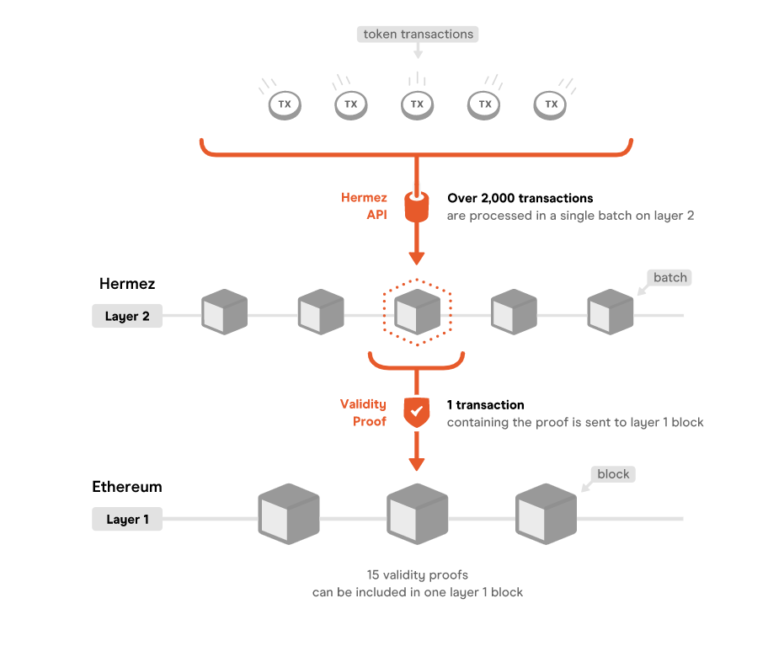
\includegraphics[width=0.5\textwidth]{rollups.png}
   \caption*{\textit{From a brief zk-Rollup explainer on \href{https://en.bitpush.news/articles/4451336}{bitpush news} by Lincoln Murr}}
\end{wrapfigure}

%\begin{figure}[H]
%    \centering
%    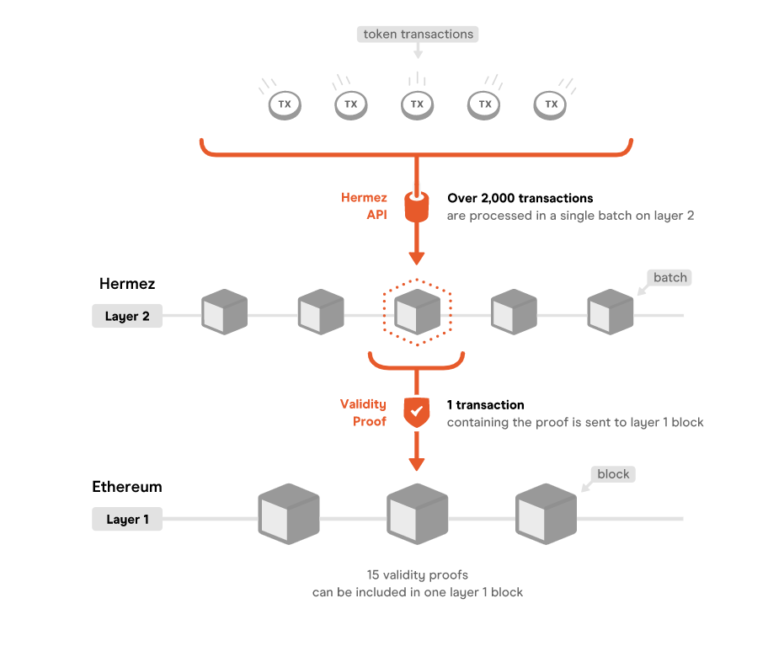
\includegraphics[width=0.65\linewidth]{rollups.png}
%    \caption{\textit{From a brief zk-Rollup explainer on \href{https://en.bitpush.news/articles/4451336}{bitpush news} by Lincoln Murr}}
%    \label{fig:enter-label}
%\end{figure}

An important property of an L2 network is that users must be able to \href{https://x.com/apoorveth/status/1981408173400740037}{permissionlessly withdraw from the Layer 2} by submitting a transaction on Ethereum L1; if users can't withdraw their funds from the L2 permissionlessly, then it is not considered a layer 2 network in the canonical sense. In this way, the Ethereum Layer 1 is able to extend (most of) its property rights to users on L2s while offering access to blockspace that is $\approx$ 10 - 100x cheaper. Here's an \href{https://x.com/donnoh_eth/status/1879210463952818472}{interesting example} of when donnoh.eth was able to force a transaction through on Sony's permissioned layer 2 network, \href{https://x.com/soneium}{Soneium}.  

There are certainly some tradeoffs when it comes to the property rights on L2s versus the L1;  \href{https://l2beat.com/scaling/summary}{L2beat} does a great job highlighting what the tradeoffs are by evaluating Rollups on a set of criteria proposed by Vitalik \href{https://ethereum-magicians.org/t/proposed-milestones-for-rollups-taking-off-training-wheels/11571}{here}. 

He described evaluating Rollups on their trust assumptions and splits them up into 3 successive stages; each stage can be thought of as being along the axis of least trustless (at risk of human intervention) to most trustless (lowest risk of human intervention). These are Stage 0, Stage 1, and Stage 2, with Stage 2 being considered the most trustless of the three stages (safest for users). 

To achieve Stage 2, a Rollup must: 
\label{Stages}

\begin{itemize}
    \item \textbf{Self Sequence:} In the event of Sequencer failure, users must be able to force transactions through to the Rollup from Ethereum L1
    \item \textbf{State validation:} If a faulty transaction was executed by the L2, anyone must be able to permissionlessly submit a fraud proof that a transaction executed by the L2 was faulty in order to revert the faulty transaction
    \item \textbf{Data Availability:} The rollup's transaction data must be posted on Ethereum L1 such that it is available for fraud proof construction
    \item \textbf{Self propose:} Anyone can permissionlessly become a block proposer to the L2 after a time period of inactivity from the whitelisted block proposers
    \item \textbf{Exit Window:} There must be a long enough delay between when  an upgrade to the rollup is proposed and when the upgrade is implemented for users to exit back to the L1 permissionlessly. This way, if the upgrade is malicious, users have enough time to permissionlessly exit the rollup to avoid the malicious upgrade. This is generally accepted to be 30 days. As of October 2025, no rollup has an upgrade delay that meets 30 days. 
\end{itemize}

\begin{figure}[h]
    \centering
    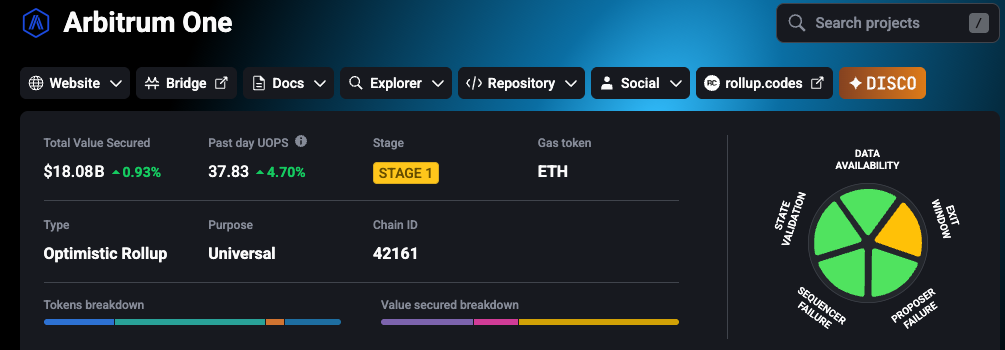
\includegraphics[width=0.9\linewidth]{slices.png}
    \caption{\textit{\href{https://l2beat.com/scaling/projects/arbitrum\#stage}{L2Beat} gives Layer 2s colored slices based on which of the above requirements are met.}}
\end{figure}

So what is the fundamental bottleneck for increasing transaction throughput on Layer 2 networks without increasing user transaction fees?\\

Ethereum's ability to host the data produced by L2s from user transactions is called \textbf{Data Availability}. Ethereum's Data Availability is limited;  Rollups that post their data to Ethereum must compete with each other for the limited space. For this reason, Ethereum's Data Availability is the fundamental bottleneck. 

\subsubsection{Increasing Data Availability Throughput for Ethereum}

\begin{wrapfigure}{r}{0.2\textwidth}
   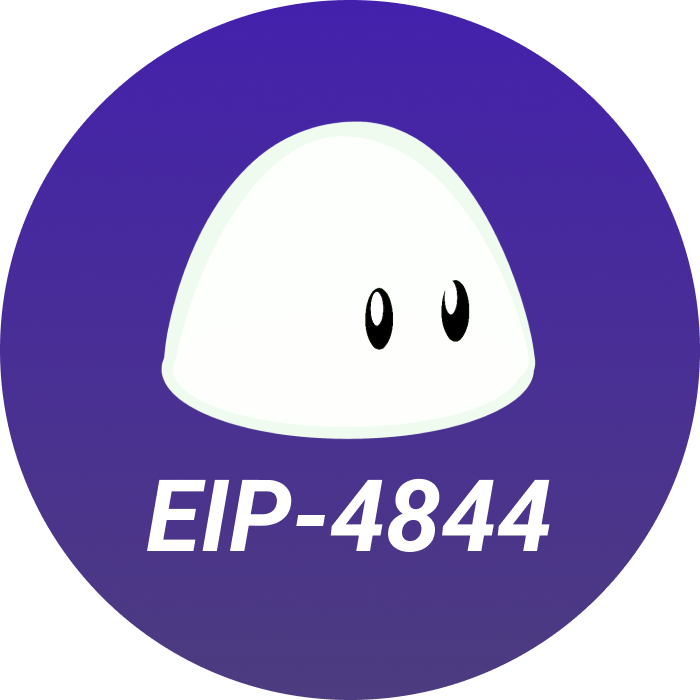
\includegraphics[width=0.2\textwidth]{blobs.png}
   \caption*{\textit{an \href{https://www.eip4844.com/\#faq}{FAQ about blobs}}}
\end{wrapfigure}

As mentioned above, L2 networks must post their data to Ethereum L1 such that it is available for anyone to verify correct transaction execution. 

Before EIP-4844, L2 networks were posting their transaction data to Ethereum's \href{https://www.quicknode.com/guides/ethereum-development/transactions/ethereum-transaction-calldata}{call data}, which is a very limited resource for storage. Call data is also expensive because it persists on the chain forever. The competition for this limited space between Rollups only exacerbated the issue. 

To address this, in \href{https://eips.ethereum.org/EIPS/eip-4844}{EIP-4844} the Ethereum community created a new transaction type for posting L2 transaction data to a ``bucket" for receiving this data, called Binary Large Objects, or ``blobs". These blobs were purpose-built for receiving L2 transaction data, with a new and \href{https://dune.com/0xRob/blobs}{separate fee market} distinct from the standard Ethereum L1 fee market, and an expiration date so they are ``pruned", or deleted, by Ethereum node operators after 4096 epochs, or approximately 18 days. Blobs must be available on L1 for long enough that they are available to anyone who wants to store them, such that Ethereum acts as a real-time \href{https://notes.ethereum.org/@vbuterin/proto_danksharding_faq#If-data-is-deleted-after-30-days-how-would-users-access-older-blobs}{``bulletin board"}, but the network itself is not responsible for storing them forever. Removing them from the network makes blob storage far cheaper than call data. 

Blobs have been extremely effective at reducing L2s' costs to post their data to L1; these savings are passed on to users. This is nicely visualized on \href{https://l2beat.com/scaling/projects/arbitrum#onchain-costs}{L2beat} for each L2, here is Arbitrum's:  

\begin{figure}[H]
    \centering
    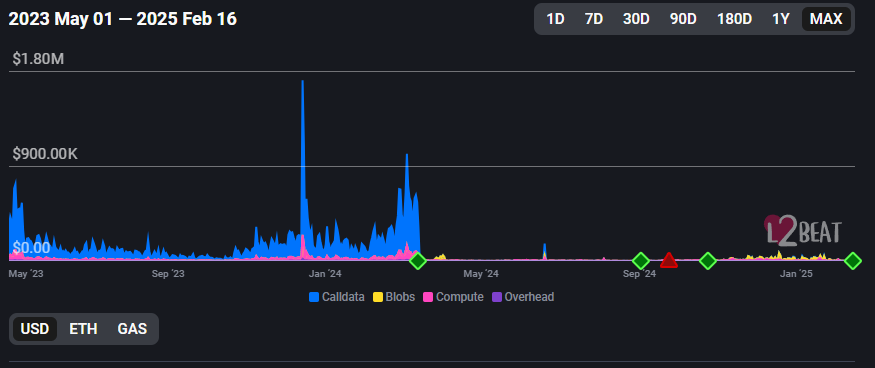
\includegraphics[width=0.8\linewidth]{blob costs.PNG}
    \caption{\textit{can you tell when Arbitrum switched from call data to blobs?}}
    \label{fig:enter-label}
\end{figure}

In order for users to enforce correct transaction execution, all of the data generated by a rollup must be available on the Layer 1. If any of this data is missing, then users will be unable to verify correct transaction execution and construct a fraud proof in case of malicious activity from the L2. Today, all validators download this data and make it available to the network in the form of blobs. 

We have created a cheaper way to store L2 transaction data, but it is still not enough! Only a maximum of 9 blobs can be posted per block on Ethereum, and the blob fee market targets a 6 blob average per block through a fee mechanism. Each blob can only be 128 kilobytes at maximum, and at 12 second block times, this means that the average data availability throughput on Ethereum is approximately 5.5 Gigabytes of space per day, not enough if Ethereum is to be the financial center of gravity for the entire globe. 

One way Ethereum can increase its data availability throughput is to simply increase the number of blobs that can be posted with each block. Ethereum did just that in its most recent upgrade, Pectra, where the blobs per block target was increased from three to six blobs per block. The effect of this change can be seen very clearly in this below chart:

\begin{figure}[H]
    \centering
    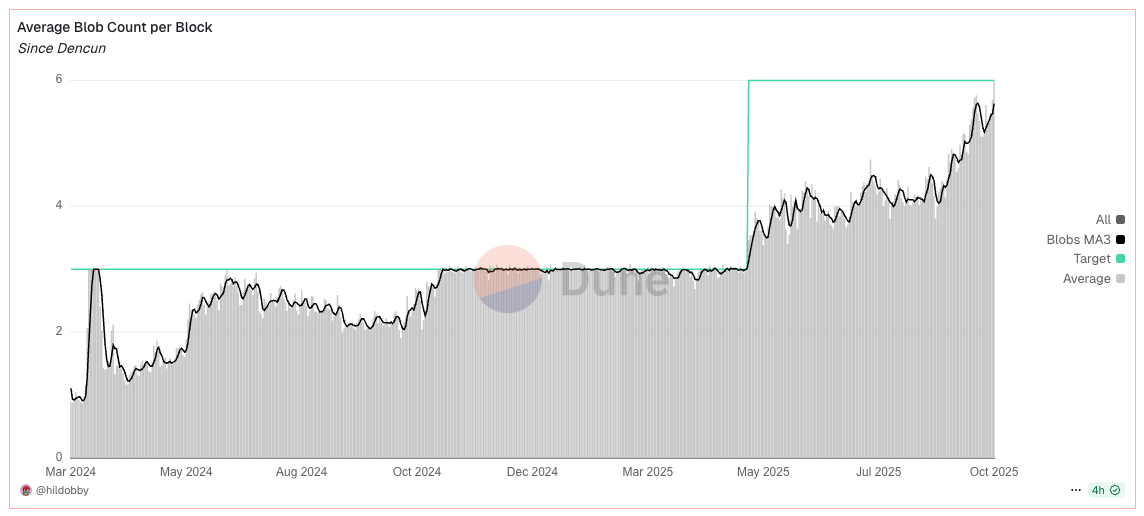
\includegraphics[width=0.8\linewidth]{blobs per block.png}
    \caption{\textit{Blob target increased from 3 to 6 blobs per block in May of 2025, chart is from Hildobby's \href{https://dune.com/hildobby/blobs}{blob dashboard}}}
    \label{fig:enter-label}
\end{figure}

With \href{https://eips.ethereum.org/EIPS/eip-7892}{EIP-7892}, Mark Mackey (\href{https://x.com/EthDreamer}{@ethDreamer}) and Raul Kripalani (\href{https://github.com/raulk}{@raulk}) have also introduced the concept of ``Blob Parameter Only" forks, in which a hard fork would only serve to increase the number of blobs per block, and nothing else. 

A challenge with continuously increasing the number of blobs per block is that the network cannot keep increasing the blobs per block indefinitely without negatively impacting the hardware requirements of becoming a validator due to the increased storage requirements of storing the blobs -  \textit{but Ethereum needs to scale even further.} How can Ethereum make even more efficient use of its blob capacity?

One way we can scale this data availability throughput further, without increasing validator hardware requirements, is through \textbf{Data Availability Sampling.}

\clearpage

\hypertarget{PeerDAS}{\subsubsection{Data Availability Sampling - PeerDAS}}
\label{PeerDAS}

\begin{wrapfigure}{r}{0.4\textwidth}
   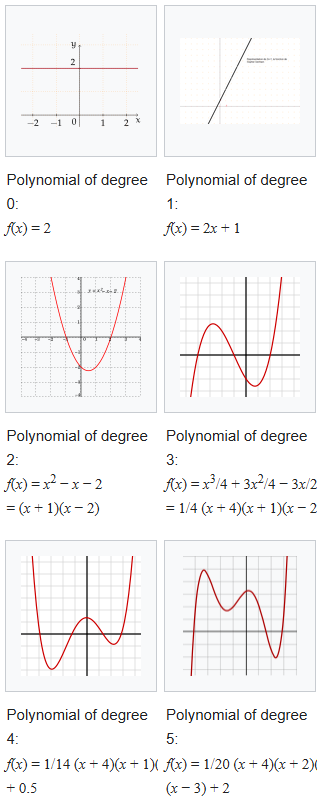
\includegraphics[width=0.4\textwidth]{polynomials.PNG}
   \caption*{polynomials of degree $n$ - image credit \href{https://en.wikipedia.org/wiki/Polynomial}{wikipedia}}
\end{wrapfigure}

Because Ethereum wants to minimize hardware requirements, and bandwidth constraints in particular, Ethereum needs to prove that all of the data is available \textit{without forcing validators to download all of the data.} To do this, validators can sample the data contained in the blobs to check for availability and can prove with an extremely high probability that all of the data is available \textit{without downloading all of it}. This is \textbf{Data Availability Sampling.}

Better yet, if any of the data is missing, Validators are able to reconstruct that missing data using \textbf{Reed Solomon Erasure Coding} \textit{as long as more than 50\% of the data is available.} Reed Solomon Erasure Coding is a way of reconstructing missing data from a data set. 

It works with the following steps:

\begin{enumerate}
    \item \textbf{Convert the transaction data into a polynomial \href{https://www.youtube.com/watch?v=bzp_q7NDdd4}{using Lagrange Interpolation:}} this is called ``encoding the data". In a finite field\footnote{Ethereum blobs would be encoded in a polynomial of degree 4096; the field is considered finite because the polynomial can only be evaluated between $0 \leq x \leq$ and some extremely large prime number, $\sim$ $2^{253}$}, this polynomial \textit{is always unique.}
    \item \textbf{Extend the data:} Evaluate the polynomial at additional data points in a finite field to ``extend" the data. This creates redundancy - we'll see why we do this in a second. 
    \item \textbf{Send the data (in the form of a polynomial) to the recipient:} In this case, this means posting the data as a blob on Ethereum L1
    \item \textbf{Reconstruct the original data:} The data in the blob can be used to reconstruct the original transaction data, \textit{even if some of the blob data is missing!} How? As long as we have more than half of the data in the blob, we know the equation for the polynomial, \textit{which we know is unique}, and we can evaluate it at the parts where data is missing to reconstruct the full blob. 
\end{enumerate}

We start by converting the transaction data into a polynomial - this is called ``encoding" the data. It works by taking advantage of the fact that polynomials of a specific order $n$ in a finite field are unique, when constructed from a data set of $n+1$ points. 

We then evaluate the polynomial at an additional set of points to extend the blob size by a factor of $2$. Extending the blob size introduces redundancy to the transaction data - if $>$ half of the blob data is known, we can determine the polynomial used to construct the blob, and the rest of the entirety of the blob can be reconstructed. The validator set propagates that block throughout the network; because we know that the original transaction data can be reconstructed as long as more than half (\textit{sidenote: it's not actually half, I'll be referring to half because its easier, but a16z does a \href{https://a16zcrypto.com/posts/article/an-overview-of-danksharding-and-a-proposal-for-improvement-of-das/}{fantastic job} breaking this down a bit more deeply if you're curious}) of the data is made available, then the Ethereum network only has to prove that more than half of the blob data is available.  

Now that the network only has to prove that \textit{half of the data is available,} we can introduce the ``Sampling" part of \textbf{Data Availability Sampling}. Each validator is assigned some pseudo-random subset of the blob data and is responsible for downloading that data, storing it, and making it available upon request. 

Since each validator is now responsible for downloading \textit{only a portion} of the full data, this greatly reduces the bandwidth requirement for each validator by a factor dependent on what fraction of the total blob data each validator is required to download. If each validator only has to sample $1/8$th of the data in each blob, then the blob count the network can include per block can be increased by a factor of 8x without increasing the amount of data each validator has to download per block on average. 

\begin{figure}
    \centering
    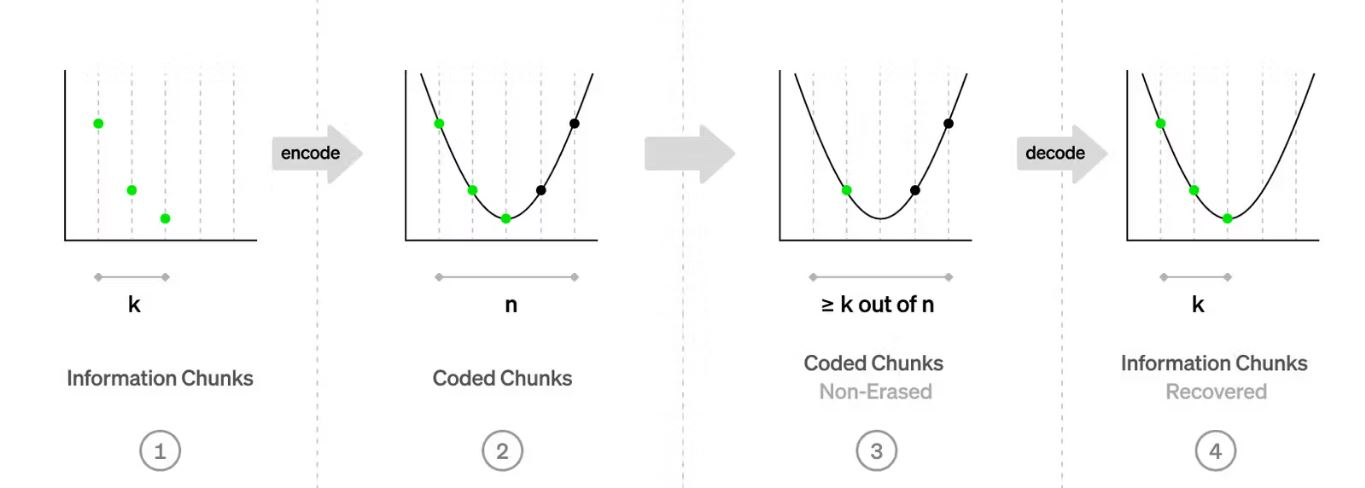
\includegraphics[width=0.9\linewidth]{paradigm DAS image.JPG}
    \caption{\textit{Here is a fantastic graphic from an \href{https://www.paradigm.xyz/2022/08/das}{article} written by \href{https://www.jneu.net/}{Joachim Neu} for Paradigm}}
    \label{fig:enter-label}
\end{figure}

Each validator is now required to make available a small portion of the total blob data, but using math, the network is able to come to consensus about whether or not all the data is available globally. Splitting up the data between the validators is called \textbf{Sharding}, since it ``shards" the data into pieces. Sharding allows the blobs which can be included in each block to be greatly increased, \textit{significantly increasing Ethereum's scalability.}

One incredibly powerful consequence of sharding is that \textit{Ethereum's scalability now increases as more validator nodes join the network!} As Ethereum is able to split the blob storage load across more Ethereum nodes, the Ethereum network is able to store more and more blob data. This can be thought of analogously to torrenting, where data is shared across many nodes. 

PeerDAS will go live in Ethereum's \href{https://forkcast.org/upgrade/fusaka}{Fusaka upgrade}, scheduled for December, 2025. The ultimate goal is to target an average throughput of 128 blobs per block and a maximum of 256 blobs per block. This amount of data throughput is estimated to be able to support up to $\sim$90k TPS. 

\begin{center}
        (125 kilobytes/blob * 128 blobs/block) / (180 bytes per ERC20 transfer) = $\sim$90k transactions per block
\end{center}

As activity on Ethereum's constellation of Layer 2s continues to increase, we may get to the point where layer 2s are burning significant amounts of Ether. This \href{https://ethereum-blob-simulator.netlify.app/}{blob burn simulator}, made by \href{https://x.com/timjrobinson}{Tim Robinson}, allows you to play with your assumptions to figure out how much ETH will be burned, assuming a certain amount of aggregate activity across all rollups. 

How can we improve the transactions per second even further? By reducing the amount of data required for each transaction. The best way to describe this is the following diagram: 

\begin{figure}[H]
    \centering
    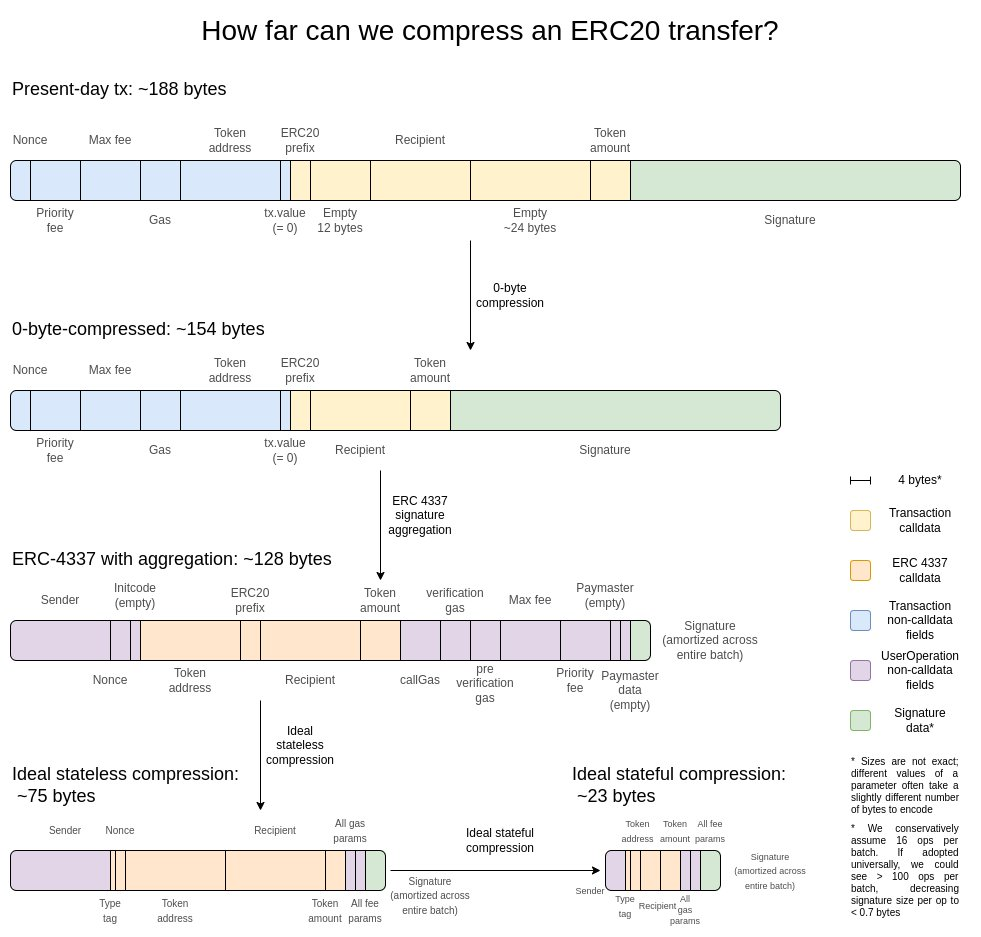
\includegraphics[width=0.7\linewidth]{erc20 data compression.jpg}
    \caption{\textit{reducing erc20 transfer data requirements, Vitalik's original 
\href{https://x.com/VitalikButerin/status/1554983955182809088}{tweet}}}
\end{figure}

By reducing the amount of data required per transaction, we can increase the maximum transactions per second of the chain. 

\begin{comment}
\subsubsection{Based Rollups}

\subparagraph{A Based Rollup} is a rollup that uses the Layer 1 network that it posts its data to also for \textif{sequencing}. 

Sequencing is the process of ordering transactions submitted by users. There are various ways to order transactions submitted by users, some rollups use first come first serve, others extract \hyperref[MEV]{MEV} by reordering transactions, others use a hybrid of the two approaches. 

Many rollups run their own sequencer that is responsible for this transaction ordering. But there are drawbacks for users when a Rollup is dependent on its own sequencer; if a sequencer goes down, the rollup stops dead in its tracks.  (use grok query about times prominent sequencers have gone down; use A Based Thesis for more inspiration on centralized sequencer drawbacks here) 



define sequencing

mention the drawbacks of centralized sequencing

highlight the benefits of based sequencing and the UX challenges, which could be solved by based preconfirmations

mteam's talk on \href{https://youtu.be/_iee7LkcUeQ?si=wfOTlHdqTkAVECh0}{based rollups}

Layer 2 Rollups use sequencers to order transactions that are submitted by users. One of the challenges around sequencers on the largest layer 2 Rollups Many rollups use centralized sequencers that are responsible for ordering transactions
\end{comment}


\subsection[\protect\textbf{\small Ethereum's Execution Layer}]{Ethereum's Execution Layer}
\label{Execution Layer}

One of the ultimate goals of Ethereum as decentralized blockchain technology is enabling easy verification that the current state of the chain is the deterministic output of everything that has ever happened on that chain. At its simplest, a blockchain can be boiled down to a \textbf{State Transition Function} (STF), where the input is the current state of the blockchain and the incoming transactions, and the output is the newly updated state of the chain. As Vitalik discusses in his blog, 

\begin{align}
    S' = STF(S, B)
\end{align}

Where $S$ is the current state, $B$ is the current block, and $S'$ is the output of the state transition function (i.e. the next block). In other words, \textit{it is an accurate ledger}, and anyone can easily verify the state of the ledger is correct. 

To execute state transitions, Ethereum uses the Ethereum Virtual Machine (EVM). The EVM is a virtual environment which consists of many different \href{https://www.ethervm.io/}{low level opcodes} (e.g. addition, subtraction, multiplication, division, etc.) that combine to complete higher level logic. More generically, the set of these opcodes together is called an ``instruction set architecture", or ISA. These opcodes act sequentially on current blockchain state to produce a deterministic outcome $S'$ based on the transaction contents of a block. 

Today, each validator accesses stored blockchain state, re-executes these opcodes sequentially using the blockchain's current state, then verifies the output matches the proposed block. Because of the need to fully re-execute transactions in order to verify the state transition occurred correctly, execution and verification are intrinsically linked. 

In the future, we can \textit{decouple execution and verification} by eliminating the need for every full ethereum node to re-execute each block by instead having validators check a small (few hundred Kilobytes), lightweight mathematical proof for correctness. Getting there will require implementing \textbf{Stateless Verification} and \textbf{Validity proofs}, and will ultimately enable \textbf{Native Rollups}.

\subsubsection{Improving Ethereum's Execution Layer}

There are three main parts to improving the execution layer, their goals are:

\begin{itemize}
    \item \textbf{Stateless Verification:} Minimizing the amount of data that is needed to store the \textit{current state} of the blockchain $S$ (which today consumes hundreds of GB) and needs to be stored by fully verifying Ethereum nodes
    \item \textbf{Validity proofs:} Using mathematical proofs that are easily checked for correctness (and can even be verified on devices with limited compute, e.g. smart watches) to prove that the \textit{state transition function}, $STF( S,B)$, correctly outputs the state of the chain $S'$ after taking the current sate and the current block as an input (i.e. executing users' transactions correctly)
    \item \textbf{Native Execution:} Because validity proofs are constant size and verifying their correctness takes milliseconds, the EVM can be enshrined as a \textit{precompile}, enabling scaling increases of $>$100x on the Ethereum Layer 1
\end{itemize}

The combination of stateless verification and validity proofs unlocks native execution and enables the vision Vitalik explains succinctly at Rollup Day 2022 and Justin Drake described recently in an interview with Gelato:

\begin{center}
\textit{``My vision of the future of running an Ethereum node is... you should not need to have a piece of fancy hardware... you have your phone, you should be able to stake \$1M of ETH... on your phone if you want to... an Ethereum block might contain 3.5MB of data and a SNARK... download the 3.5MB... verify the SNARK, done. Block is correct."} - Vitalik Buterin, \href{https://youtu.be/6hfVzCWT6YI?si=cubN-8mEUoNr3n_z&t=1409}{link}
\end{center}

\begin{center}
    \textit{``...instead of the validators having to re-execute L1 blocks, they just have to verify SNARK proofs. And these SNARK proofs are constant size and constant time to verify. You just take a few milliseconds to verify, and downloading the proof is very small and constant size, so you could imagine removing the gas limit, having arbitrary large blocks, and that not mattering to the validators, because the amount of work they have to do is constant and doesn't matter what the gas limit is... we should be able to achieve 1 Gigagas per second, which is about 1,000 times more than what we have (today)."} - Justin Drake, \href{https://youtu.be/0q-qT67yyVs?si=cIWbDG-6zHFDh-hS&t=1196}{link}
\end{center}

Let's dive a bit deeper into both stateless verification, validity proofs, and native execution.  

\subsubsection{Stateless Verification}
\label{Stateless Verification}

An important part of making verification ``easy" is minimizing the hardware requirements of verifying the state, where ``state" refers to current account balances, every smart contract that has been deployed to Ethereum, data stored onchain, etcetera. Verifying the state involves starting with the initial state of the chain, referred to as ``genesis" (or a socially propagated checkpoint to prevent long range attacks)\footnote{Weak subjectivity involves establishing checkpoints to eliminate the threat of long range attacks, read more \href{https://ethereum.org/en/developers/docs/consensus-mechanisms/pos/weak-subjectivity/}{here}}, and re-executing every transaction that has occurred onchain to verify that you got the same result as everyone else. Today, this requires a large amount of data which grows every day. The ultimate goal of \textbf{stateless verification} is to use mathematical proofs that are easily verifiable to prove Ethereum's state \textit{without needing to download all of Ethereum's state data}, which today is close to (2TB) and grows in size at approximately 30GB per year. This data is stored in a \href{https://www.alchemy.com/docs/tree-data-structures}{``tree"} format.\footnote{Shoutout to \href{https://x.com/Alchemy}{Alchemy} for the fantastic four part series on data storage in Ethereum in their section on cryptography basics you can find \href{https://www.alchemy.com/docs/tree-data-structures}{here}} Trees are used in computer science to store data efficiently for data management and retrieval. 

Blockchains store and retrieve data with every change to state, so it is important to both minimize the time it takes to retrieve data from the set, as well as minimize the total amount of data storage needed for the blockchain to function. Today in Ethereum, this data is stored in the form of a Merkle PATRICIA trie, MPT for short, (generally pronounced ``try", short for re\textit{trie}val - all tries are trees, but not all trees are tries; 
 PATRICIA being short for Practical Algorithm to Retrieve Information Coded in Alphanumeric), which is a special type of search tree. 

\begin{wrapfigure}{r}{0.6\textwidth}
   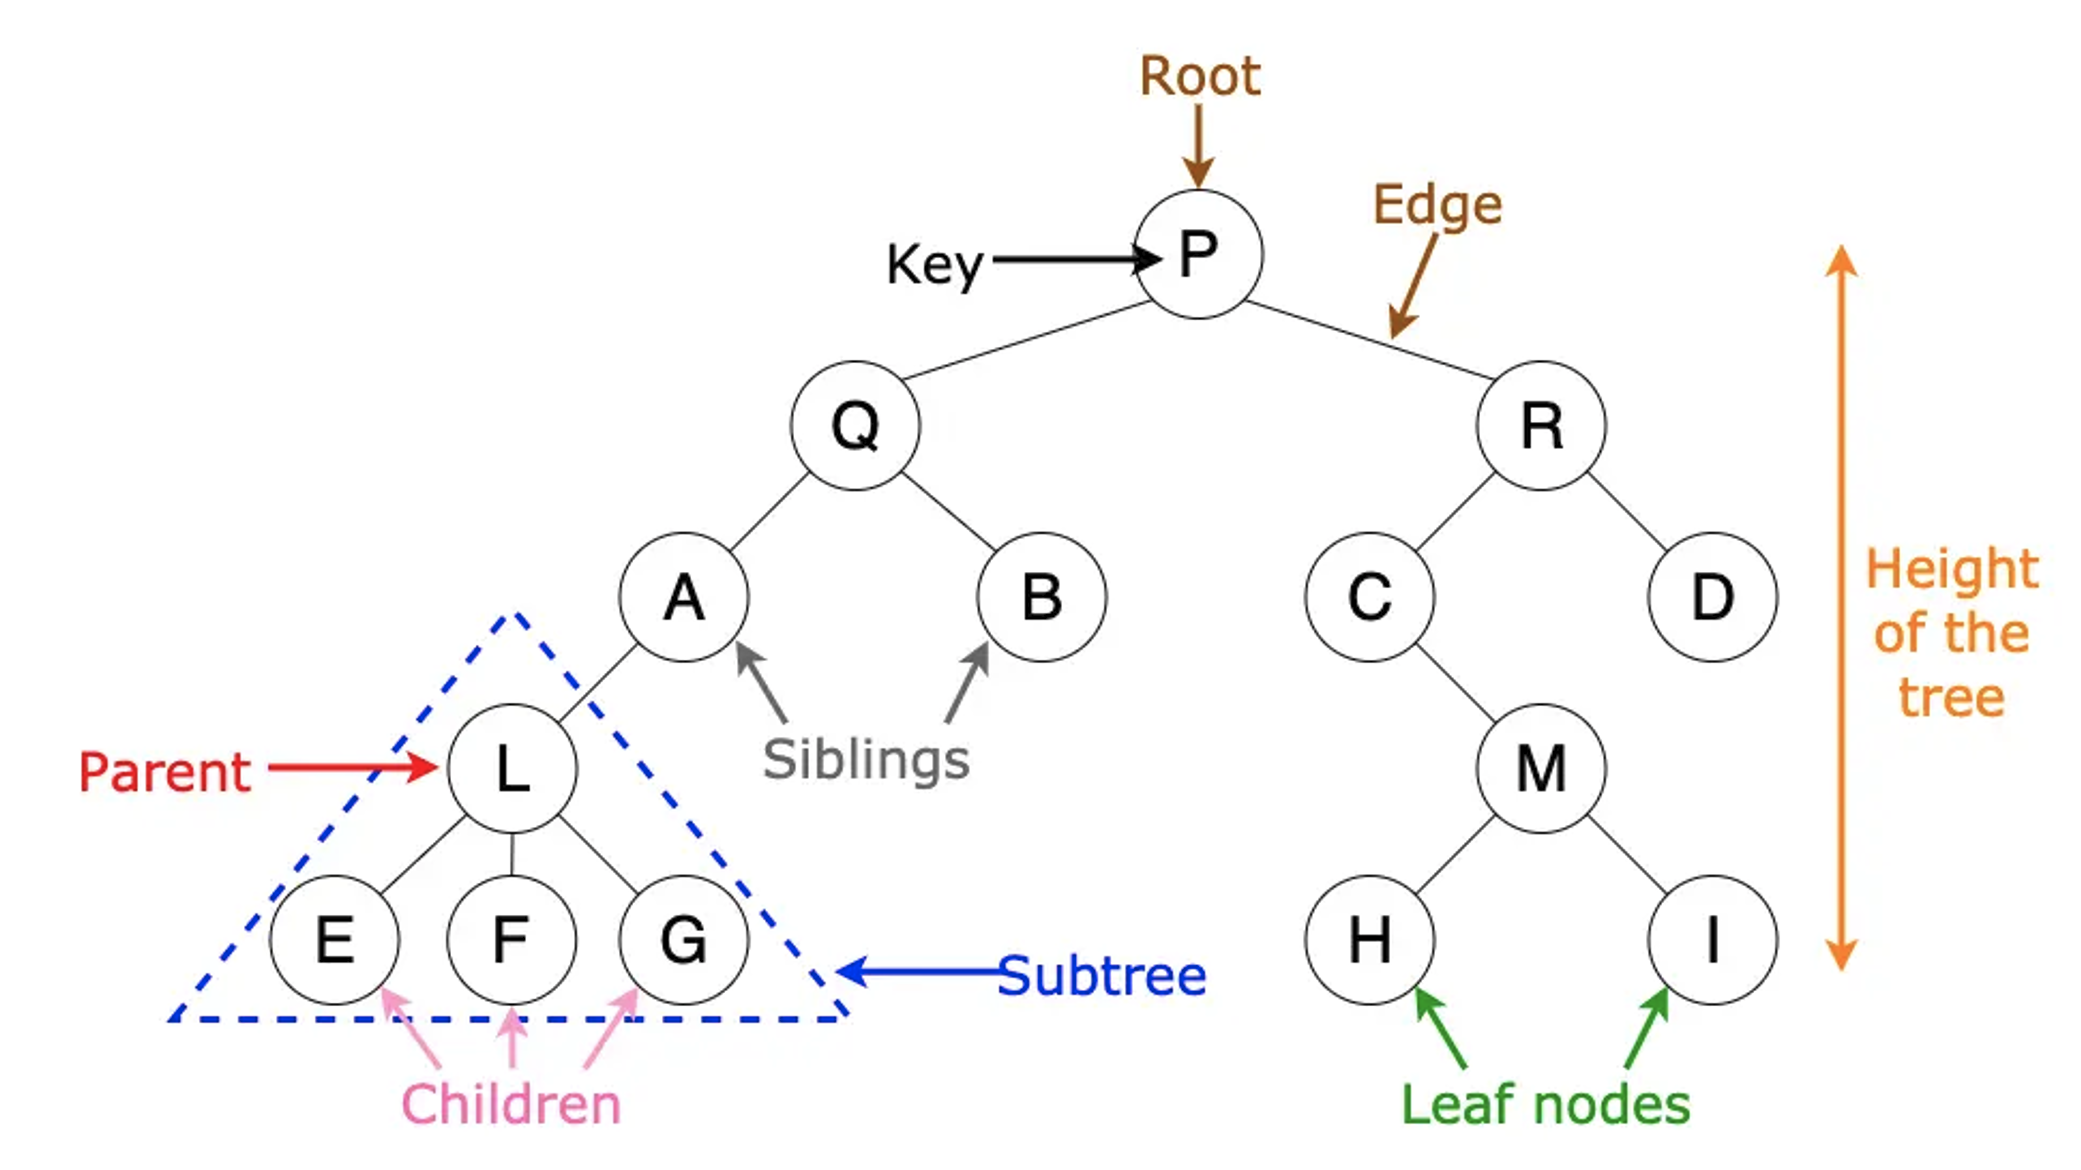
\includegraphics[width=0.6\textwidth]{tree.PNG}
   \caption*{\textit{A Tree Diagram from \href{https://www.alchemy.com/docs/tree-data-structures}{Alchemy's docs}}}
\end{wrapfigure}

Let's break down what makes Ethereum's search tree both a ``Merkle" and a ``PATRICIA trie". Ethereum's data structure is considered \textbf{Merkle} because of how the integrity of the contents of the trie are verified - using hashes. In the context of verifying state, the advantage of this architecture is that it becomes easy for anyone to verify transaction ``D" exists in the block without even needing the entire contents of the block, by calculating the hash of the root using only hash of D, hash of C and D together (R), and hashing Q+R; if the result is different than the expected result, we know that \textit{something} is different between the two data structures we are comparing (i.e. your local view of the contents of that block versus the network's view, as a simple example), even if the difference is extremely small. 

\begin{wrapfigure}{r}{0.5\textwidth}
   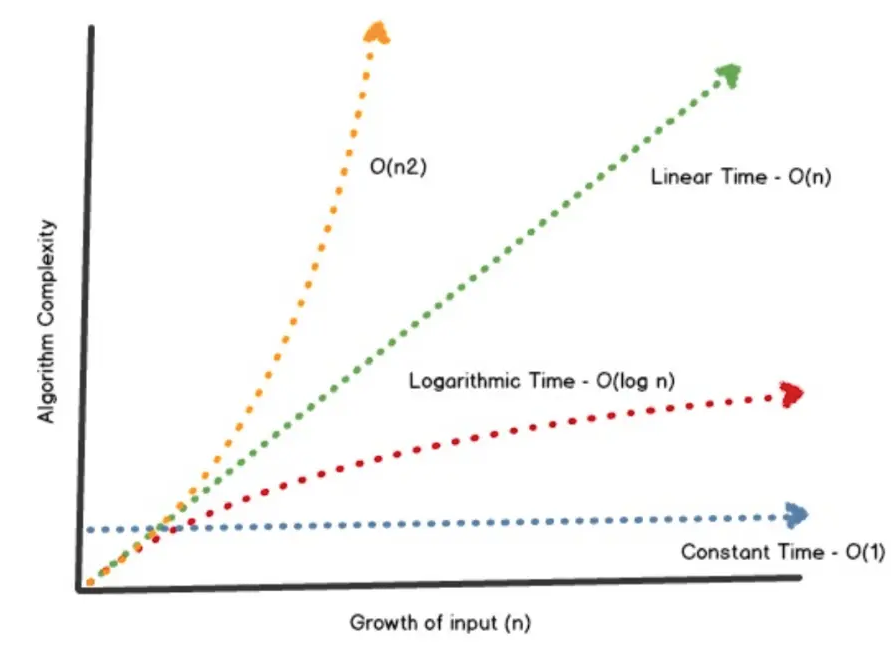
\includegraphics[width=0.5\textwidth]{time complexity.PNG}
   \caption*{\textit{Also from \href{https://www.alchemy.com/docs/tree-data-structures}{Alchemy's docs}}}
\end{wrapfigure}

Ethereum's trie is described as \textbf{PATRICIA} because it is organized such that shared prefixes are not stored more than once (this is called prefix based), meaning that all Ethereum addresses starting with ``0x1..." are stored under the same branch. This reduces both the amount of data storage required to store state and the retrieval time. Ethereum's MPT is hexary, meaning each branch of the state tree can have 16 children. 

Retrieving data from data structures for verification requires both \textit{time} and the \textit{data itself}. \href{https://en.wikipedia.org/wiki/Time_complexity}{Time complexity} is the relationship between how long it takes to search a specific data structure relative to the growth of its input size \textit{n}; \href{https://en.wikipedia.org/wiki/Space_complexity}{space complexity} is a similar concept, but instead focuses on minimizing storage required by storing data efficiently, such as in an MPT structure. Space and time complexity are expressed using big \textit{``O"} notation, with the function in the parentheses representing the relationship between the growth of the size of the input and the length of time it takes to compute the output, or the amount of storage space required. MPTs are considered fairly efficient, with the time it takes to search the tree \textit{O(log(n))}. 

Even though the MPT is considered relatively space and time efficient, state verification can be improved much further using the concept of a \textbf{``witness"}. A witness enables \textbf{stateless verification} and consists of two parts: 

\begin{itemize}
    \item the data that will be accessed in order to execute this state change (account balances, contract code, storage slots, for ex.)
    \item a cryptographic proof that the data accessed from prior state is correct
\end{itemize}

Utilizing witness data for verification of state transitions significantly reduces bandwidth and storage requirements compared to re-executing the raw state transitions; instead of needing the current full state data, only the witness data and the very computationally light step of verifying the correctness of the downloaded proof is needed, which is now approximately two orders of magnitude smaller than the state itself! 

Unfortunately, MPTs are fundamentally \textit{unfriendly} to cryptographic proofs  (and by extension producing witnesses, Vitalik explains briefly why  \href{https://vitalik.eth.limo/general/2024/10/23/futures4.html\#:~:text=of\%20the\%20MPT\%3A-,It\%27s,-a\%20hexary\%20tree}{here}), so Ethereum will need to move away from MPT to a new state tree structure that is more friendly to cryptographic proof construction. 

\subsubsubsection{Moving away from MPT: Verkle Trees versus STARKed Binary Hash Trees}

There are two approaches that are being considered, with positives and drawbacks to both. 

\begin{itemize}
    \item \textbf{Verkle Trees} - Just as in my section on \hyperlink{PeerDAS}{PeerDAS}, Verkle Trees take advantage of Elliptic Curve Cryptography to generate a concise proof, called a vector commitment, where a mathematical proof is constructed from the contents of the state tree being accessed for this particular state transition; this proof is much smaller than the original data itself. 
    \item \textbf{STARKed Binary Hash Trees} - This approach involves switching away from a hexary Merkle tree to a binary Merkle tree (each branch of the state tree only has two children instead of 16), generating the witness data (which itself is a proof), and then generating a STARK proof (Scalable Transparent Argument of Knowledge, or STARK for short) of the witness data (yes - a proof of a proof!). The STARK proof is what gets downloaded by the validator set running light clients, which is now a very small amount of data and easily checked for validity with a very small amount of computational power. 
\end{itemize}

If Ethereum wants to transition to relying on \textbf{witnesses}, then it must select one of these two approaches. \\

\begin{minipage}[t]{0.48\textwidth} % Left minipage (slightly less than 0.5 to account for spacing)
\textbf{Verkle Trees:}

\begin{itemize}
    \item[] \textit{Advantages} inlude:
\end{itemize}

    \begin{enumerate}
        \item More mature than STARK proofs, implementation would be simpler and faster
        \item Verkle proofs are updateable, which can use useful for proving the validity of transactions in the mempool and Inclusion Lists before they are propagated to the rest of the network
    \end{enumerate}

\begin{itemize}
    \item[] \textit{Disadvantages} include:
\end{itemize}

\begin{enumerate}
    \item Elliptic curves cryptography is \textit{not} quantum resistant, so switching to Verkle trees means potentially risking additional hard forks down the road to harden the chain against quantum computers
\end{enumerate}
    
\end{minipage}\hfill % Horizontal fill for separation
\begin{minipage}[t]{0.48\textwidth} % Right minipage
\textbf{STARKed Binary Trees:}

\begin{itemize}
    \item[] \textit{Advantages} inlude:
\end{itemize}

    \begin{enumerate}
        \item STARKs over hash functions add quantum resistance
        \item Can reduce full node sync time relative to Verkle trees
        \item STARKs compress witness data and have a fixed size overhead, minimizing validator bandwidth requirements even further
    \end{enumerate}

\begin{itemize}
    \item[] \textit{Disadvantages} include:
\end{itemize}

    \begin{enumerate}
        \item Limitation becomes the computation time needed to generate the STARK proof of the witness data

    \end{enumerate}
    
\end{minipage}\\
\\
\\
Regardless of which track is chosen, both approaches reduce state storage requirements by roughly \textit{two orders of magnitude} (100x); fully verifying clients would only need a few GB of storage and could be done on a mobile device. The ultimate goal for \textbf{stateless verification} is efficient access to and proof of current state, by downloading a lightweight mathematical proof and checking its validity. 

If I had to take an educated guess, I would bet that the Ethereum community comes to consensus around a STARKed binary hash tree for state storage due to its quantum resistant properties. 

\subsubsection{Validity Proofs and zkVMs}
\label{Validity Proofs}

Validity Proofs involve proving the state transition itself. The goal is to first prove current state (using \textbf{stateless verification}) and then to prove \textit{the state transition occurred correctly} (processing users' transactions correctly) without needing to re-execute onchain transactions locally by verifying lightweight, compact mathematical proofs, an operation that can be done on devices with very limited compute. Justin Drake has been explicit that the goal is to even be able to do this on devices as computationally limited as smart watches; he has referred to this as ``\href{https://youtu.be/8mJDt8TGebc?si=pN0WVLy1tBWHoFDs&t=1224}{feather staking}". Once feather staking becomes possible, almost any device with any amount of compute power would be sufficient for running a validator, making Ethereum validation much more accessible. This is not possible today because validators must re-execute every transaction on the blockchain to check for validity. 

The key unlock validity proofs allows is we can \textit{massively increase the block gas limit}. Gas is a unit of measurement of the computational effort required to execute transactions using the state transition function. The validator set has a limited amount of compute and storage, so a fee mechanism is used to limit consumption of those resources. This fee mechanism sets a price for each computational unit, called the \textit{gas price}. Gas is consumed when users pay transaction fees and the transaction fee is denominated in Gigawei per gas, or one billionth of one Ether. 

\begin{figure}[H]
    \centering
    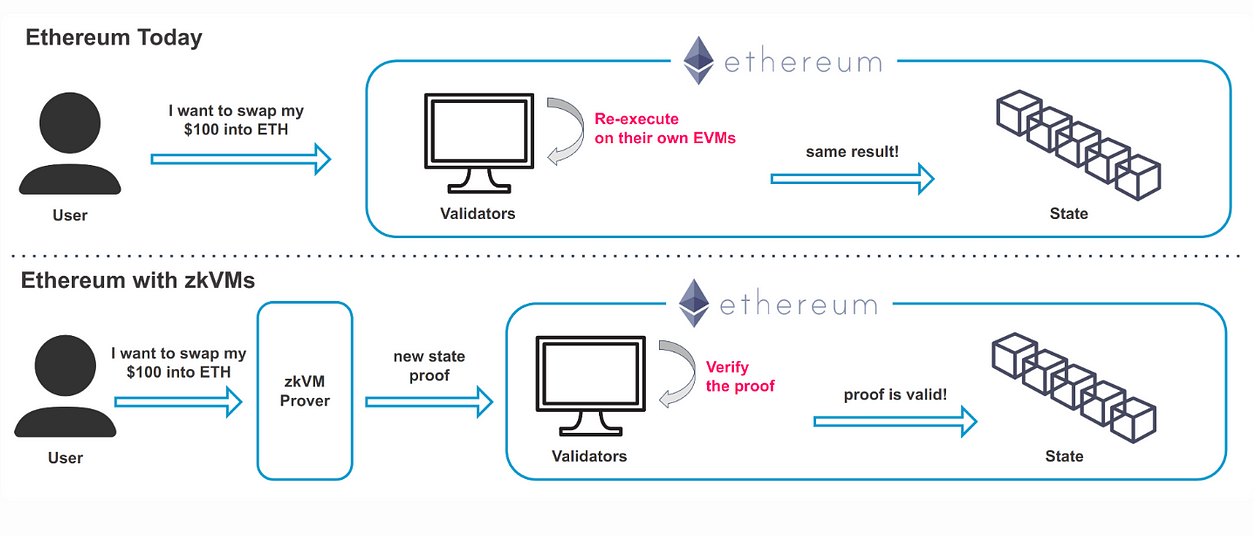
\includegraphics[width=0.9\linewidth]{zkVMs.png}
    \caption{\textit{from this \href{https://fenbushicapital.medium.com/benchmarking-zkvms-current-state-and-prospects-ba859b44f560}{deep dive} on zkVMs by Fenbushi Capital}}
\end{figure}

Verifying validity proofs are valid is constant time to verify, meaning that it is \textit{independent of the complexity of the block execution that it is proving}. Validators can prove the correctness of the proof and know the state transition occurred correctly without needing to re-execute the contents of the block themselves. This then means that the gas limit has no impact to the validator set, and the fundamental bottleneck becomes the length of time it takes to generate proofs of the block execution, which is a problem the validator set would not have to deal with.  

There are a few engineering challenges associated with validity proofs, but all seem solvable. From easier to more involved: 

\begin{itemize}
    \item \textbf{Proof generation} will require beefy hardware and validators with limited compute can't generate them. Who generates the proofs?
    \item \textbf{Replacing the EVM} will be a requirement. The EVM is not friendly to proof generation - just like the Merkle PATRICIA tree, it will have to be swapped out for something that is significantly easier to generate zero-knowledge proofs of. Vitalik \href{https://ethereum-magicians.org/t/long-term-l1-execution-layer-proposal-replace-the-evm-with-risc-v/23617}{proposed swapping out the EVM} in favor of RISC-V (pronounced risk five). 
\end{itemize}

\subparagraph{Who generates the proofs?}

In my estimation, the ``simplest" problem here is the crypto-economic problem of - ``who will generate the proofs?" While it's true that checking the validity of these proofs will be done reliably on a mobile device by a decentralized validator set, generating the proofs themselves will still need to be completed by a relatively beefy piece of hardware. 

This is an active area of development; there are a couple of different approaches that are in consideration, that are not necessarily exclusive to each other. \href{https://ethresear.ch/u/Julian/summary}{Julian} has been fairly active on this topic and has been involved in writing proposals that look at this problem from a few different angles. 

One \href{https://ethresear.ch/t/prover-killers-killer-you-build-it-you-prove-it/22308}{approach} involves making it the responsibility of the block builder for that block to provide a validity proof along with the block. This eliminates the concern around ``prover killers", in which it was possible for an attacker to grief a prover by intentionally generating a block that is expensive to prove. Another, potentially complimentary approach, would be to establish a ``prize contract" where block builders could deposit a prize for proof generation, to be paid out to who ever permissionlessly provided the proof in the following block. This might be useful for block builders who don't want to or can't be involved in proof generation.  

\subparagraph{Replacing the EVM with RISC-V} Another challenge around validity proofs involves the time it takes to generate block proofs. 

In order for proof generation to be practical, it needs to happen inside of a $\approx$ \href{https://blog.ethereum.org/2025/07/10/realtime-proving#:~:text=With%20the%20current%20slot%20time%20of%2012%20seconds%20and%20maximum%20time%20to%20propagate%20data%20across%20the%20network%20of%20~1.5%20seconds%2C%20realtime%20means%2010%20seconds%20or%20less.}{10 second time frame}, and ideally within 4 seconds. Unfortunately, the EVM is fundamentally unfriendly to proof generation, because of its \href{https://faizannehal.medium.com/understanding-the-stack-based-architecture-of-evm-af45dc9819f2}{stack based architecture}, and its 256 bit-word architecture, which just means that the EVM requires every input to be 256 bits (even true/false values are padded with zeros to 256 bits!). ZK proofs are generated over finite fields (generally 64-bits) that are smaller than 256 bits, to optimize for 64-bit operations on GPUs, requiring each input to the EVM to be split into chunks, adding significant overhead. 

One creative way to relax this 10 second constraint on proof generation is to delay generating the stateRoot of the block by one slot, as proposed in \href{https://eips.ethereum.org/EIPS/eip-7862}{EIP-7862}. This would allow an additional $\approx$ 12 seconds for proof generation. 

To avoid the need to generate proofs of the EVM directly, many zkEVM teams take the approach of converting the EVM instruction set to another, simpler instruction set called RISC-V through an interpreter, which causes a massive slowdown of \href{https://x.com/pumatheuma/status/1915541516128600348}{approximately 50-800x}. Despite this significant slowdown, it is still faster than trying to prove the EVM directly. To address this, Vitalik \href{https://ethereum-magicians.org/t/long-term-l1-execution-layer-proposal-replace-the-evm-with-risc-v/23617}{proposed} eliminating the overhead of converting EVM instructions to RISC-V by replacing the EVM with the RISC-V instruction set. As \href{https://x.com/0xJaehaerys}{jaehaerys.eth} explains in this excellent \href{https://x.com/0xJaehaerys/status/1960051628129865918}{article}, RISC-V has a series of advantages: 

\begin{itemize}
    \item it has a formal specification that is machine readable, unlike the EVM
    \item much smaller, simpler set of low level opcodes ($\approx$ 47 versus the EVM's $\approx$ 140) 
    \item RISC-V has an open ecosystem with mature tooling and supports 64-bit operations, which can fit in the finite fields used for zero-knowledge proofs
\end{itemize} 

This transition will likely \href{https://vitalik.eth.limo/general/2025/05/03/simplel1.html#:~:text=the%20following%20process%20for%20a%20VM%20change}{happen in stages}, will result in making proof generation practical, and will ultimately enable \href{https://x.com/0xJaehaerys/status/1944859201291083887}{orders of magnitude increases in scaling} of Ethereum L1. Because validators will no longer be responsible for block execution, but instead will \textit{only be responsible for checking validity proofs that are fixed in size regardless of the contents of the block being proved}, the gas limit can be increased significantly. Justin Drake even believes Ethereum can \href{https://www.youtube.com/watch?v=yvP39-EOADU}{reach 10 Million aggregate TPS by 2035}. For more on the state of validity proofs, \href{https://ethproofs.org/}{ethproofs.org} shows a dashboard of block proving times, costs, and trust assumptions associated with each of the different zkVMs.

\subparagraph{But how do we know zero-knowledge proofs are not ``proving" invalid inputs?} To be confident enough to protect hundreds of billions in value, we must be confident they won't \href{https://blog.lambdaclass.com/responsible-disclosure-of-an-exploit-in-succincts-sp1-zkvm-found-in-partnership-with-3mi-labs-and-aligned-which-arises-from-the-interaction-of-two-distinct-security-vulnerabilities/}{``prove" something that is invalid.} 

Analogous to client diversity in Ethereum L1, one approach to this problem involves having \href{https://www.youtube.com/watch?v=6hfVzCWT6YI}{multiple provers}, where more than one prover generates proofs of block execution and a super majority of the provers establishes consensus. This can be thought of in an analogous way to client diversity in L1 Ethereum, where having multiple clients establishes redundancy and resilience due to the fact that clients are built in different software languages by different teams with different approaches. The likelihood these clients will exhibit overlapping failure modes is extremely minimal, ensuring \href{https://ethereumuptime.org/}{100\% up-time} for Ethereum. 

Validity Proofs, because they are so simple to verify, allow massively increasing the gas limit of Ethereum Layer 1. A validator receives a SNARK proof that proves the state transition occurred correctly in the block, and verifies the proof is correct \textit{without needing to re-execute the contents of the block}.  

As a consequence of the massively increased gas limits, the EVM can be enshrined as a \textit{precompile}, enabling \textit{Native Rollups}.

\subsubsection{Native Rollups}
\label{Native Rollups}

Validity proofs are the technological innovation that make Native Execution practical. 

Validity proofs remove the gas limit as a bottleneck, allowing an arbitrary amount of transactions to be included in each Ethereum L1 block. This unlocks \textit{Native Execution}, which involves enshrining the execution layer's state transition function, i.e. the EVM, as a \textit{precompile}. Layer 2 networks can then call this precompile, which is essentially an input/output function that is by construction equivalent to the EVM's state transition function. 

Rollups that take advantage of this new precompile will be called \textit{Native Rollups}. Native Rollups have significant advantages over non-native rollups, namely around reducing attack vectors for users, simplicity of development, and forward compatibility with Ethereum L1. \href{https://x.com/pumatheuma}{Uma Roy}, CEO of \href{https://x.com/SuccinctLabs}{Succinct Labs} developing a leading zkVM, and Justin Drake do a fantastic job \href{https://youtu.be/0TOnHHnB6Ro?si=dZFF5jDdiLCUE4ou}{breaking this down} in a Bankless interview. \\

Native Rollups have the following advantages over non-native rollups: 

\subparagraph{They no longer need to develop their own state transition funciton, and no longer need fraud proof infrastructure.}

In the Bankless interview with Uma and Justin, David does a great job \href{https://youtu.be/0TOnHHnB6Ro?si=7UiKfIUPfdSi_Wuk&t=1827}{revisiting} the concept of Rollup \hyperref[Stages]{stages}, in which there are five requirements for rollups. One of those requirements involves having \href{https://l2beat.com/scaling/projects/arbitrum#state-validation}{very complex} fraud proof infrastructure that would allow a user to prove a faulty state transition occurred and revert it. \begin{wrapfigure}{r}{0.3\textwidth}
   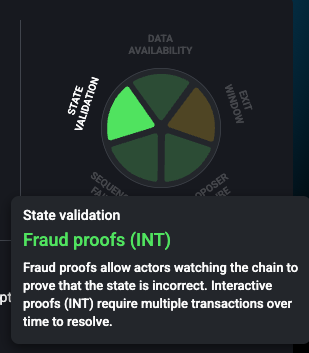
\includegraphics[width=0.3\textwidth]{pie slice.png}
   \caption*{\textit{State Validation is removed as a risk vector for users, graphic of Arbitrum's current stage 1 progress, from \href{https://l2beat.com/scaling/projects/arbitrum}{L2Beat}}}
\end{wrapfigure} If a Rollup becomes native by relying on the enshrined EVM precompile, that state transition becomes canonical by definition, \textit{making the fraud proof infrastructure unnecessary.} 



\textit{This removes a risk surface for users} - they can be confident the state transition occurred in compliance with the EVM. As David puts it nicely, \textit{"With Native Rollups, we just eliminate that slice (state validation) entirely."} Governance risks disappear as security councils become obviated as well. 

\begin{center}
    \textit{"(Layer 2s require)... prover networks, there's watchtowers in the case of fraud proof games, there's security councils, all of that ancillary infrastructure just collapses to one line of code where you're just calling the precompile. So not only is it a massive security improvement, it's a massive simplicity improvement as well."} - Justin Drake
\end{center}

\subparagraph{This also removes a significant source of overhead for rollup development, making rollup deployment far simpler.} Native Rollups can skip the development overhead of the fraud proof and challenge infrastructure \textit{because their state transition function is EVM equivalent by construction,} making native rollup development far faster and cheaper. 

\subparagraph{Native Rollups will be forward compatible with Ethereum Layer 1.} As the EVM changes, non-native rollups are required to keep pace with these changes in order to stay EVM equivalent, if that is their goal. By contrast, Native Rollups \textit{don't need to do this,} as the EVM precompile will be upgraded by Layer 1 Ethereum. 

For more on Native Rollups, L2Beat put together a great resource on Native Rollups \href{https://native-rollups.l2beat.com/}{here.} This \href{https://medium.com/l2beat/native-rollups-where-they-are-and-where-they-are-going-cb21eb103d46}{article} titled \textit{"Native Rollups: Where they are, and where they are going"}, a collaboration between Donnoh.eth from L2Beat and \href{https://x.com/ConorMcMenamin9}{Conor McMenamin} from the \href{https://x.com/NethermindEth}{Nethermind} client team, does a fantastic job exploring where Native Rollups are today and the tradeoff space between throughput and composability for different Native Rollups that are looking to interoperate. Donnoh also gave a \href{https://youtu.be/0O3JyJpMQLQ?si=6sAghjK242mx0W1t}{talk} on Native Rollups at Token 2049 just a few weeks ago where he gives the background and highlights their fantastic benefits, including their potential for 10M aggregate TPS between L1 + L2s, verifiable on a smart watch! Justin Drake mentions \href{https://x.com/drakefjustin/status/1978435449489158312}{here} that zkEVMs will ultimately allow a 100x in Ethereum L1 scaling and that there will be an update on progress for proof generation at Devconnect in November 2025. 

\subsection{\textbf{MEV, ETH Issuance, and Quantum Resistance}}

These three research directions did not fit neatly in to the Execution, Data, and Consensus buckets, but are critical none the less. 

\subsubsection{Minimizing the Centralizing Effects of MEV}

\begin{center}
    ``One of the biggest risks to the Ethereum L1 is proof-of-stake centralizing due to economic pressures." - Vitalik Buterin
\end{center}

Left unchecked, economies of scale are an existential threat to \textit{every} L1 blockchain and Ethereum is no exception. Economies of scale are a centralization vector for the protocol; the bigger you are, the faster you grow relative to the competition. In the limit, ie over long enough time horizons, this can cause problems with the core functioning of the protocol. 

Ethereum's most pressing threats from centralization currently revolve around MEV and its rate of issuance of new Ether from staking rewards. 

Ethereum is successful when Ethereum preserves decentralized block validation and robust censorship resistance, as Vitalik describes:

\begin{center}
    ``We get a chain where block production is... centralized, but block validation is trustless and highly decentralized, and specialized anti-censorship magic prevents the block producers from censoring." - Vitalik Buterin, \href{https://vitalik.eth.limo/general/2021/12/06/endgame.html}{``Endgame"}
\end{center}

Mike Neuder does a fantastic job making this more explicit in his \href{https://ethresear.ch/t/mechan-stein-alt-franken-ism/20321}{``Mechan-stein"} post (more on this below), where he describes the three properties we want to preserve: 

\begin{itemize}
    \item \textbf{A Competitive Builder Market} \verb|->| \textbf{Property 1: } We want to make the market for the right to order transactions (MEV extraction) as \textit{transparent and competitive as possible.}
    \item \textbf{Block validation remains decentralized (and thus trust-minimized)} \verb|->| \textbf{Property 2: } By ensuring the attester role remains as simple as possible, we can ensure that block validation, the process of achieving consensus, remains as accessible, decentralized, and credibly neutral as possible. 
    \item \textbf{The chain is censorship resistant} \verb|->| \textbf{Property 3: } Ensuring that transactions cannot be excluded from the chain. 
\end{itemize}
\label{Properties}


Let's start with outlining one of the centralizing forces Ethereum faces first, MEV, and then we can discuss how to minimize its impact. 

\subsubsubsection{What is Maximum Extractable Value (MEV)?}
\label{MEV}

Maximum Extractable Value (MEV), formerly Miner Extractable Value in the days of Proof of Work, in a general sense is when some form of onchain value is available to be arbitraged, generally through a transaction ordering mechanism, by a sophisticated actor who is able to take advantage of a less sophisticated user that submitted a transaction. A really simple example in the Proof of Work days might have been if a user tries to execute an arbitrage trade that would net them \$1000, but a miner who became aware of that trade from the public mempool before it gets included in a block replaces that transaction with their own, taking the \$1000 reward for themselves. In this toy example, the miner was able to use their privileged knowledge of incoming order flow and put their transaction ahead of the user's. An early post from user pcmgoohan on \href{https://www.reddit.com/r/ethereum/comments/2d84yv/miners_frontrunning/}{reddit} describes this problem well. \href{https://x.com/bertcmiller}{Bert Miller} from Flashbots wrote a very entertaining \href{https://x.com/bertcmiller/status/1402665992422047747}{series of posts} about MEV that is absolutely worth your time; he is known for popularizing the MEV landscape as the \href{https://bertcmiller.com/glimpse.html}{dark forest}. 

\textbf{MEV is a centralizing force.} One way we know MEV is a specialized field and a centralizing force is that we can see a \href{https://en.wikipedia.org/wiki/Pareto_distribution}{Pareto Distribution} of the top MEV bots on Ethereum listed by total profit: \\

\begin{figure}[H]
    \centering
    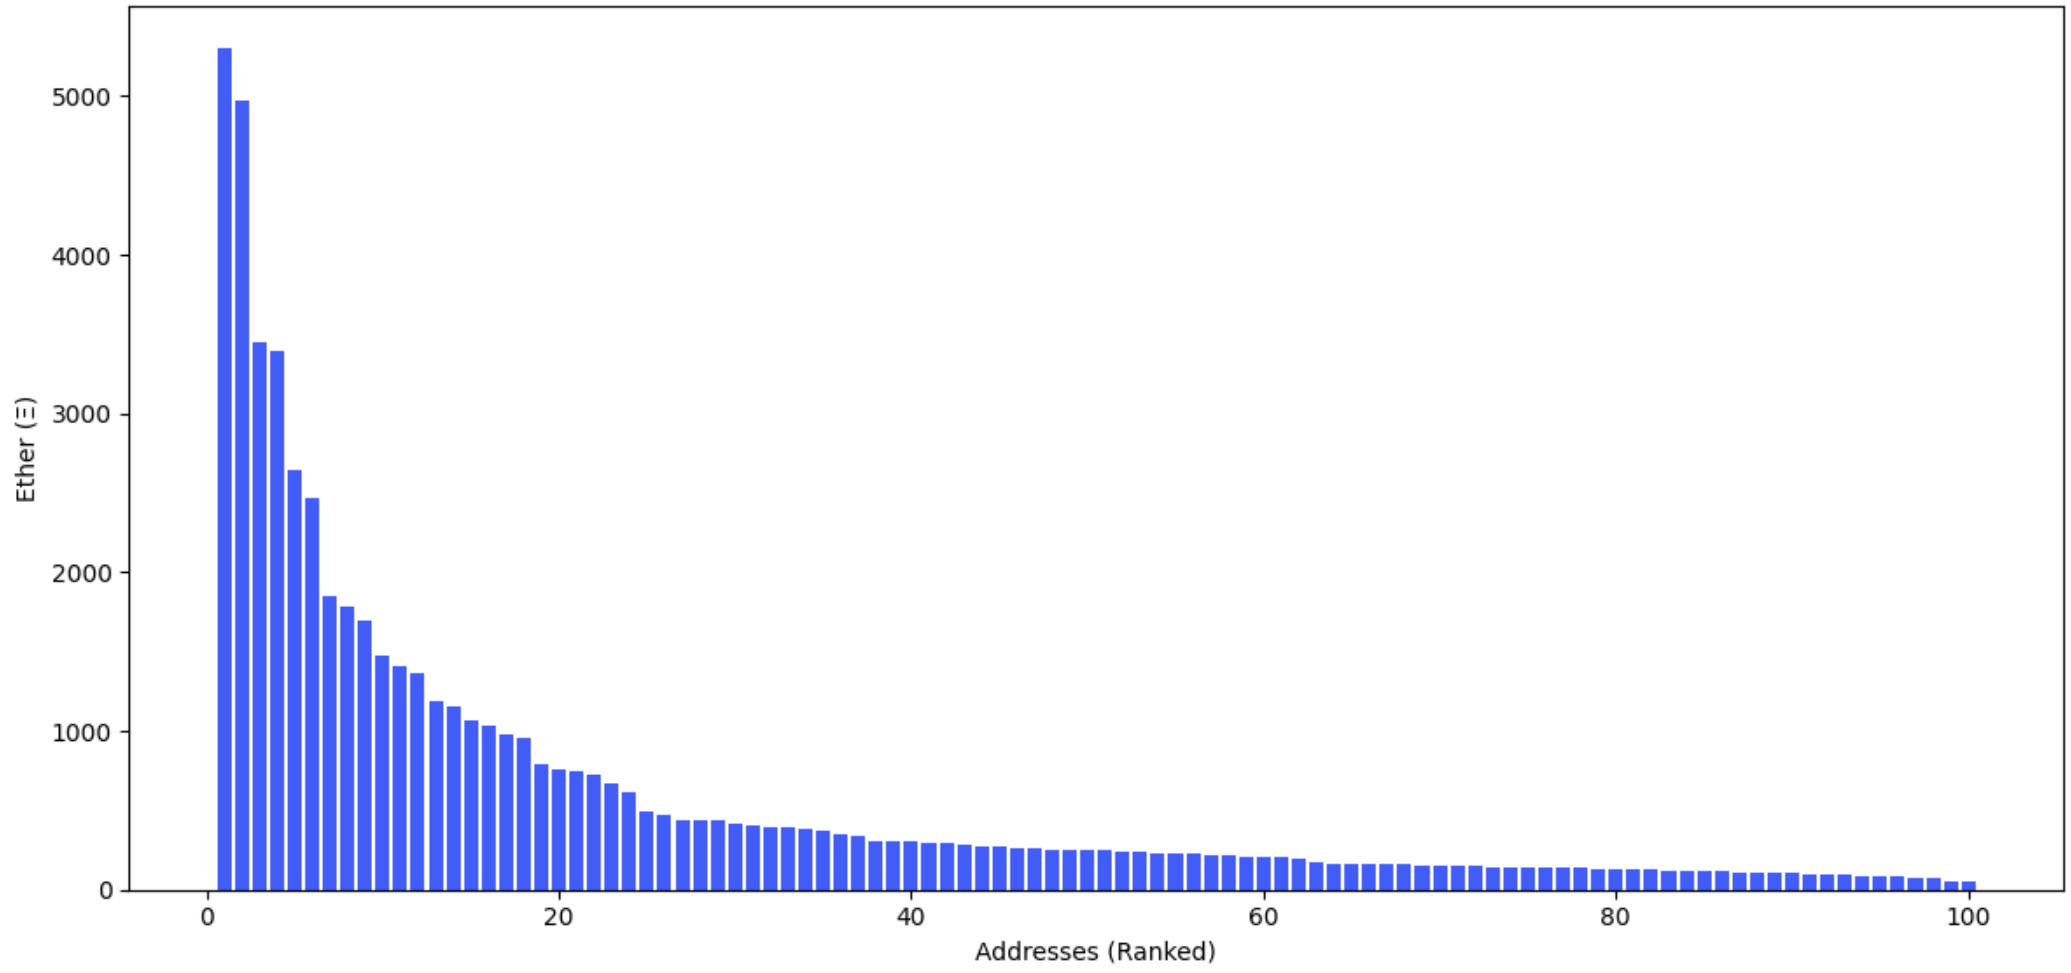
\includegraphics[width=0.9\linewidth]{MEV pareto distribution.PNG}
    \caption{\textit{A (not exhaustive) graphic Distribution of MEV bot profits I generated, data is from \href{https://libmev.com/leaderboard}{libmev.com} by \href{https://x.com/crypticwoods_}{@cripticwoods\_}}}
\end{figure}

The best performing MEV bots have an advantage over the competition; this advantage gives the highest performers the ability to go after even the tiniest profit opportunities with extremely slim profit margins, allowing them to capture opportunities that are not available to less performant MEV bots. These advantages then compound - creating the pareto distribution we see above. 

\begin{figure}[H]
    \centering
    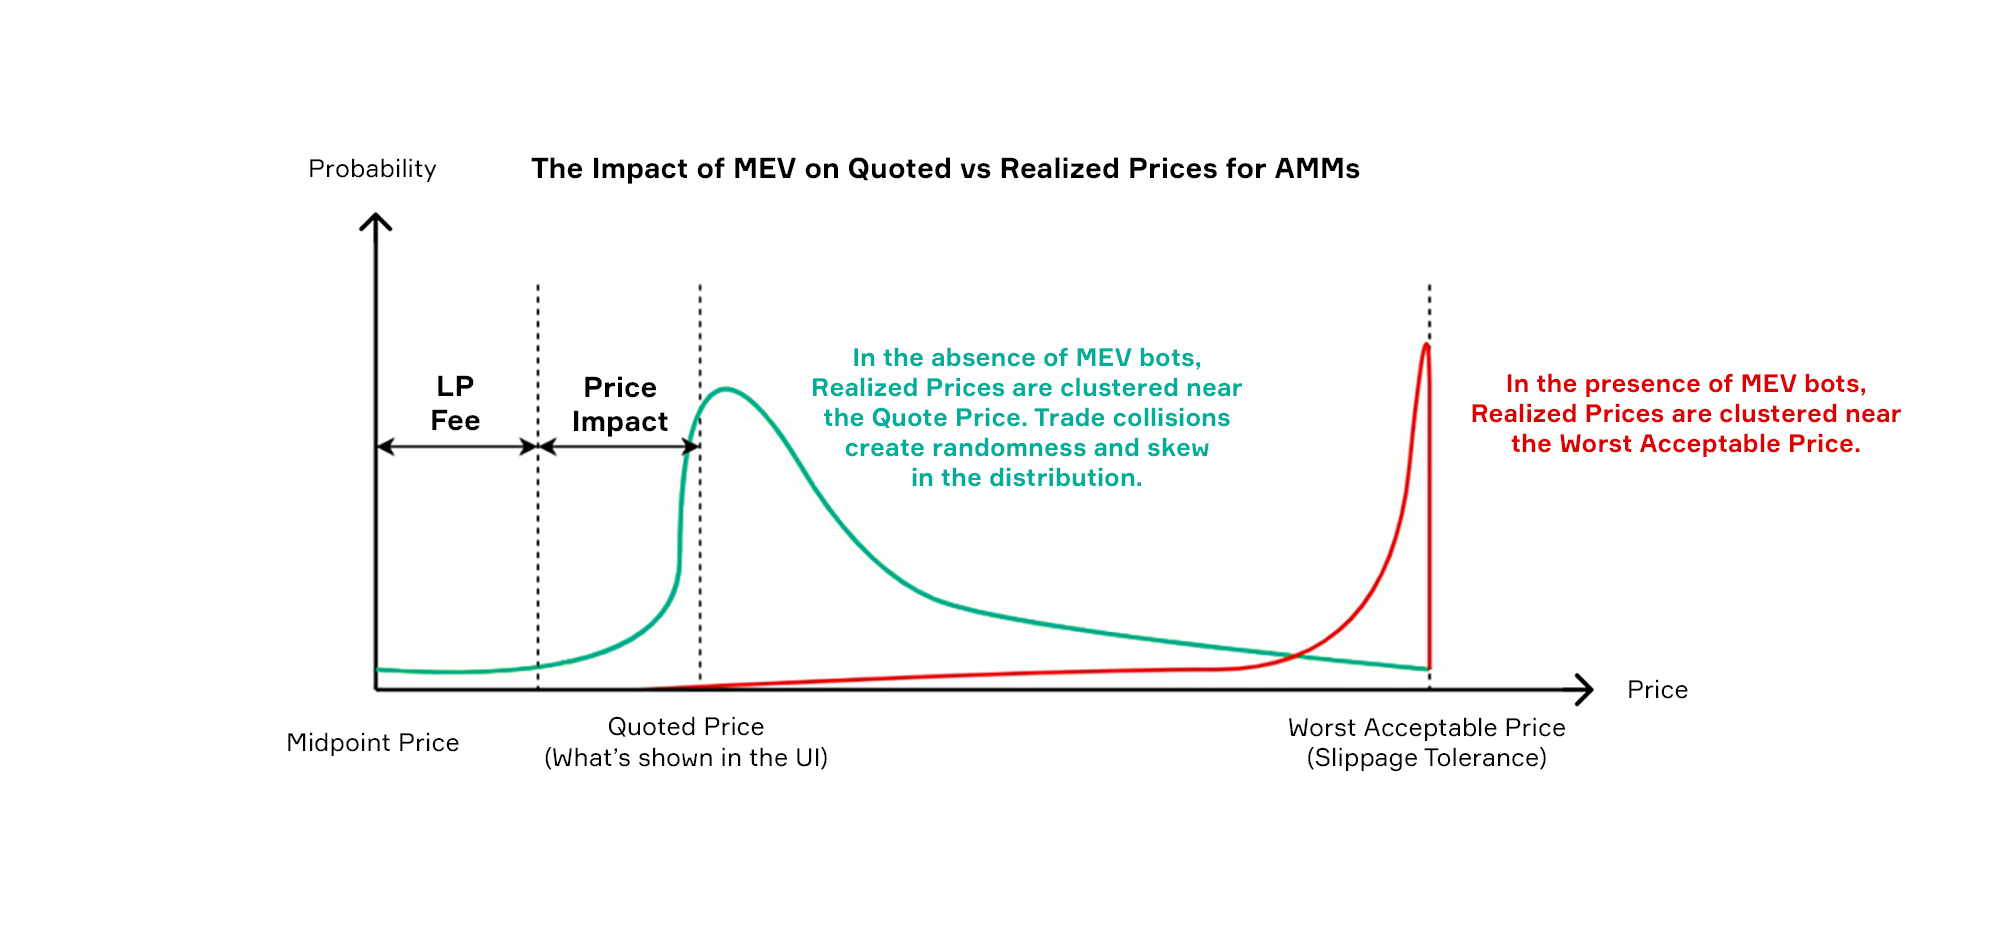
\includegraphics[width=0.9\linewidth]{MEV bot slippage.png}
    \caption{\textit{Your slippage is MEV bots' opportunity, read more on 0x.org \href{https://0x.org/post/measuring-the-impact-of-hidden-dex-costs}{here}}}
\end{figure}

While MEV does have some positive impacts on the ecosystem - mainly around maintaining an efficient market across trading platforms, such as CEX/DEX arbitrage - MEV does also have some serious negative externalities. It can mean worse trade execution for the small guy and pushes gas costs up on Ethereum L1 due to the sheer amount of activity of MEV bots. Most alarmingly, in the PoW days, MEV rewards were far larger than the block reward from mining; this dynamic incentivized attackers to rent compute power and reorganize the chain in their favor - a threat to consensus! The seminal paper called \href{https://arxiv.org/pdf/1904.05234}{\textit{Flash Boys 2.0: Frontrunning, Transaction Reordering, and Consensus Instability in Decentralized Exchanges}} sought to quantify MEV and describe these threats to decentralized consensus. Due to MEV acting as a vector for centralization and the potential threats to consensus due to MEV driven incentives to reorg the chain, the Ethereum community has realized that minimizing the impact of MEV is important to the long term survival of Ethereum. 

\subparagraph{\textit{How do we minimize the centralizing effects of MEV?}}



As I see it, minimizing MEV involves two components. The first is to \textbf{make the market for MEV as competitive as possible.} Making the MEV market more competitive means there are more actors earning MEV at a slower rate, which slows down the rate of centralization of sophisticated actors. \href{https://x.com/phildaian}{Phil Daian}, one of the authors of the Flashboys 2.0 paper mentioned earlier, went on to found \href{https://www.flashbots.net/}{Flashbots}, a company that has made it its mission to democratize MEV - or, put another way, make the market for MEV more accessible, increasing the number of competitive participants. 

\clearpage

\begin{comment}
\begin{wrapfigure}{r}{0.5\textwidth}
  \begin{minipage}{0.45\textwidth}    % Slightly smaller than wrapfigure width to avoid overflow
    \quad\quad\quad\quad\quad\large \textit{Combatting MEV}
    \begin{enumerate}
      \item \normalsize\textbf{make the competition for MEV as competitive as possible:} MEV is often referred to as the \href{https://bertcmiller.com/glimpse.html}{``the dark forest".} Making more market participants more aware of existing opportunities increases competition for those opportunities and erodes competitive edges. [link to Flashbots inspect and any other tools that help illuminate the forest?]
      \item \textbf{isolate the validator set from centralizing forces:} Unbundle functions so that market sophistication can be ``contained" into specific sectors that we are ``okay" with if they centralize (link to vitalik's post on this topic). Provide examples of market functions and what is actually being unbundled. Where are we going? 
      \item \textbf{Maintain censorship resistance through the centralization-resistant attester layer (ie Inclusion lists).} \textit{This is the goal.} 
    \end{enumerate}
  \end{minipage}
\end{wrapfigure}
\end{comment}

\begin{aside}
   \textit{An aside worth mentioning:} It's important to understand that today the validator set is responsible for two main functions. 
   
   \begin{enumerate}
       \item \textbf{Block proposals:} This part is relatively easy to understand - validators build blocks locally by aggregating transactions from the public mempool, place them in order of transaction fee, and propose them to the network for inclusion. Alternatively, a validator can select a block that has been built for them by the specialized builder market and served to them through a \href{https://beaconcha.in/relays#t7d}{relay}, which has a much higher chance of maximizing their payout from execution layer rewards. \href{https://docs.flashbots.net/flashbots-mev-boost/introduction#:~:text=%E2%80%8B,from%20a%20marketplace%20of%20builders.}{MEV-Boost} serves as the infrastructure mechanism to establish the relationship between validators and the block builders who compete in an auction. You can think of this as an out of protocol implementation of ``Proposer Builder Separation" - more on PBS in a bit. 
       \item \textbf{Attestations:} Attestations consist of two parts, one forward looking and one backward looking. The forward looking piece is responsible for selecting the next consensus block, aka ``the head of the chain", via the \href{https://eth2book.info/capella/part2/consensus/lmd_ghost/}{LMD-GHOST} fork choice rule. The backward looking piece finalizes blocks, forever cementing them into the chain at the risk of economic loss from a large portion (specifically, a minimum of 1/3rd) of the validator set. This is done via the  \href{https://eth2book.info/capella/part2/consensus/casper_ffg/}{Casper the Friendly Finality Gadget} mechanism. The combination of these two mechanisms form Ethereum's Proof of Stake consensus protocol. 
   \end{enumerate}

\end{aside}

The second component involves a realistic understanding that \textit{centralizing forces will always exist in markets.} In lieu of completely eliminating it, the key for Ethereum is to isolate the centralizing effects of MEV \textit{away from the set of attesters.} 

\subsubsubsection{Isolating the Attester Set - Achieving \hyperref[Properties]{Properties 1 \& 2}}

As \href{https://x.com/barnabemonnot}{Barnabe} describes in his post, Ethereum \href{https://mirror.xyz/barnab%C3%A9.eth/QJ6W0mmyOwjec-2zuH6lZb0iEI2aYFB9gE-LHWIMzjQ}{ has given} validators the right to both propose blocks and attest to them, establishing the network's consensus. 

The problem with this is that today, Ethereum validators \textit{are the sole entity with the right to include transactions and in which particular order to include them in} via the block proposal mechanism. Because optimizing economic value (and extraction) from a block is such a high skill endeavor (read: requires powerful hardware, proprietary algorithms, and requires capital), the block building market suffers from centralization. \href{https://www.youtube.com/watch?v=69IZIIsanvM}{In a talk at Devcon}, Jonah Burian says the centralizing effect of MEV is due to the monopoly proposers have (validators today) over the right to order and include transactions when proposing blocks. 

\begin{wrapfigure}{r}{0.3\textwidth}
   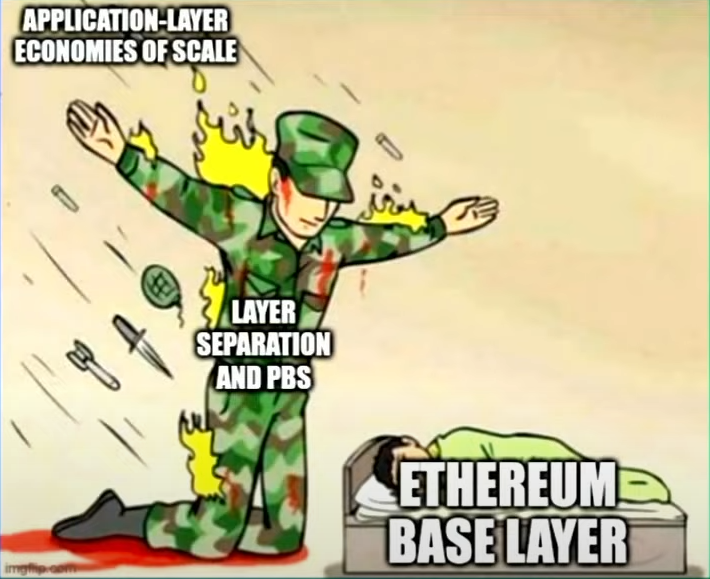
\includegraphics[width=0.3\textwidth]{insulating L1.PNG}
   \caption*{\textit{\href{https://www.youtube.com/watch?v=OD54WfVuDWw}{Devconnect Amsterdam}, 2022}}
\end{wrapfigure}

Due to this high skill requirement, most validators sell their right to transaction ordering using \href{https://docs.flashbots.net/flashbots-mev-boost/introduction}{MEV-Boost}. MEV-Boost is an optional piece of software that runs in tandem with traditional Ethereum consensus and execution layer clients, called a sidecar. MEV-Boost was developed by Flashbots and it gives validators the ability to auction off their right to order transactions in a block to block builders who specialize in maximizing value extraction from blocks via optimal transaction ordering, in exchange for the higher rewards that come with the optimized transaction ordering. \href{https://x.com/nero_eth}{Toni} from the Ethereum Foundation has a \href{https://mevboost.pics/}{great dashboard} focused on MEV-Boost.  

MEV-Boost greatly increases competition in the block building market; the reason for this is that block builders are willing to pay \textit{almost} all of their earnings to compete for the right to build the block. More competition means lower margins for builders, which has the effect of slowing centralization, relative to the world where MEV-Boost does not exist, a world where we would see an opaque, private order flow to a small subset of validators develop. 

\begin{figure}[H]
    \centering
    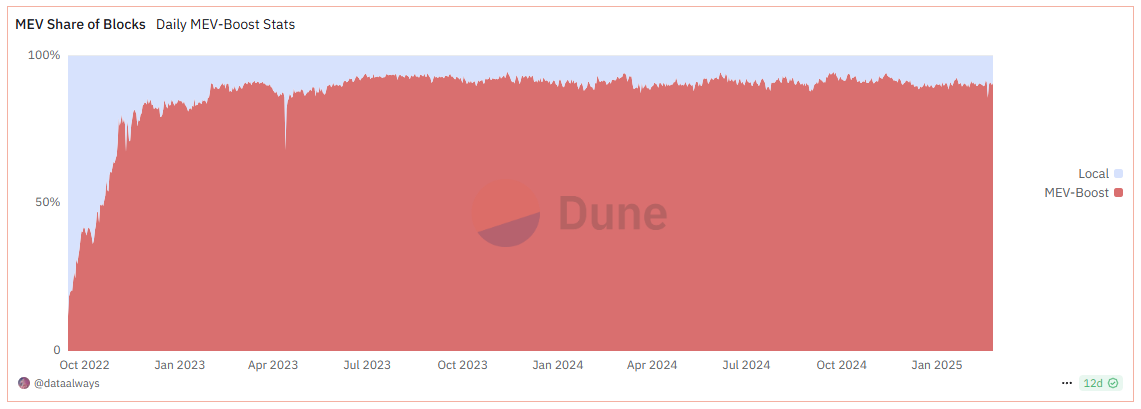
\includegraphics[width=0.9\linewidth]{MEVBoost share.PNG}
    \caption{\textit{MEV-Boost adoption share over time, by \href{https://x.com/Data_Always}{@Data\_Always}}}
\end{figure}

This \href{https://dune.com/dataalways/staking}{dashboard} on Dune by \href{https://x.com/Data_Always}{@Data\_Always} does a fantastic job illustrating graphically that about 90\% of validators use MEV-Boost to sell their transaction ordering rights - a clear indication that block builders who specialize in extracting value from optimizing transaction ordering inside blocks are far better at doing so than vanilla validators who build their blocks themselves. 

MEV-Boost makes MEV extraction more \textit{accessible and transparent} by obviating the need for trusted, private channels for block delivery from the builder market to block proposers. This helps to democratize access to MEV revenue more evenly across the validator set. 

Although validators are both block proposers and attesters, what we really care about is \textit{preventing centralization at the attester layer}. If the set of attesters suffers from centralizing forces, then the chain's consensus can be co-opted by a few privileged actors, and would be at risk of manipulation from a small number of privileged entities. The logical conclusion is to \textit{insulate the attester role from the effects of MEV}. 

\begin{center}
    \textit{The key to isolating the attester set from the centralizing effects of MEV is to simply have validators auction off their block building rights to the market of specialized block builders.}  
\end{center}

In this way, validators no longer have to compete in the competitive block building market, and can just collect \textit{most} of the MEV earnings without needing to have sophisticated software and hardware. Validators who sell these block building rights earn most of the MEV earnings, because block builders are competing with each other in an auction to pay validators more than other block builders. 

MEV-Boost does a great job allowing block proposers to auction their block building rights to the block building market today, but it is extra-protocol and involves some trust assumptions between the proposer and the block builders. The next step is to enshrine this relationship into the core Ethereum protocol to make it trustless. \href{https://eips.ethereum.org/EIPS/eip-7732}{EIP-7732}, enshrined Proposer-Builder Separation (ePBS), aims to do exactly this. ePBS is targeted for \href{https://forkcast.org/upgrade/glamsterdam}{Glamsterdam} in 2026. 

So, if we can prevent centralization at the attester layer by breaking the functions of the MEV pipeline into its constituent parts \textbf{\textit{and insulating the attester set}} \textbf{\textit{away from the parts that centralize}}, then we can minimize the threat from MEV by preventing any actor from achieving undue influence over Ethereum consensus, which would result in losing its credible neutrality and/or censorship resistance.  

By having the set of attesters sell their rights to propose blocks, this approach aims to achieve our first two properties from the beginning of this section. 

\subsubsubsection{Censorship Resistance - Achieving Property 3}
\label{Censorship Resistance}

Now that we believe we can achieve the first two properties, the last piece we need is ensuring we can maintain censorship resistance even with a centralized block building market. Centralization of block builders is not as much a threat to Ethereum as centralization of the set of attesters \textit{as long as block builders cannot censor transactions}. 

The mechanism for ensuring censorship resistance with a centralized builder market that benefits from economies of scale would work by \textit{holding this small set of centralized block builders accountable} in a crypto-economic sense if they don't include transactions. The primary effort around holding builders accountable involves the concept of \textbf{Inclusions Lists (ILs)} in this proposal called \href{https://ethresear.ch/t/fork-choice-enforced-inclusion-lists-focil-a-simple-committee-based-inclusion-list-proposal/19870}{FOCIL}, or Fork-Choice enforced Inclusion Lists, put forward by \href{https://x.com/soispoke}{soispoke}. Here is the \href{https://eips.ethereum.org/EIPS/eip-7805}{more formal EIP-7805} write up for FOCIL; it is being \href{https://forkcast.org/upgrade/glamsterdam#eip-7805}{Considered For Inclusion} in Glamsterdam as of October 2025. 

\begin{wrapfigure}{r}{0.5\textwidth}
   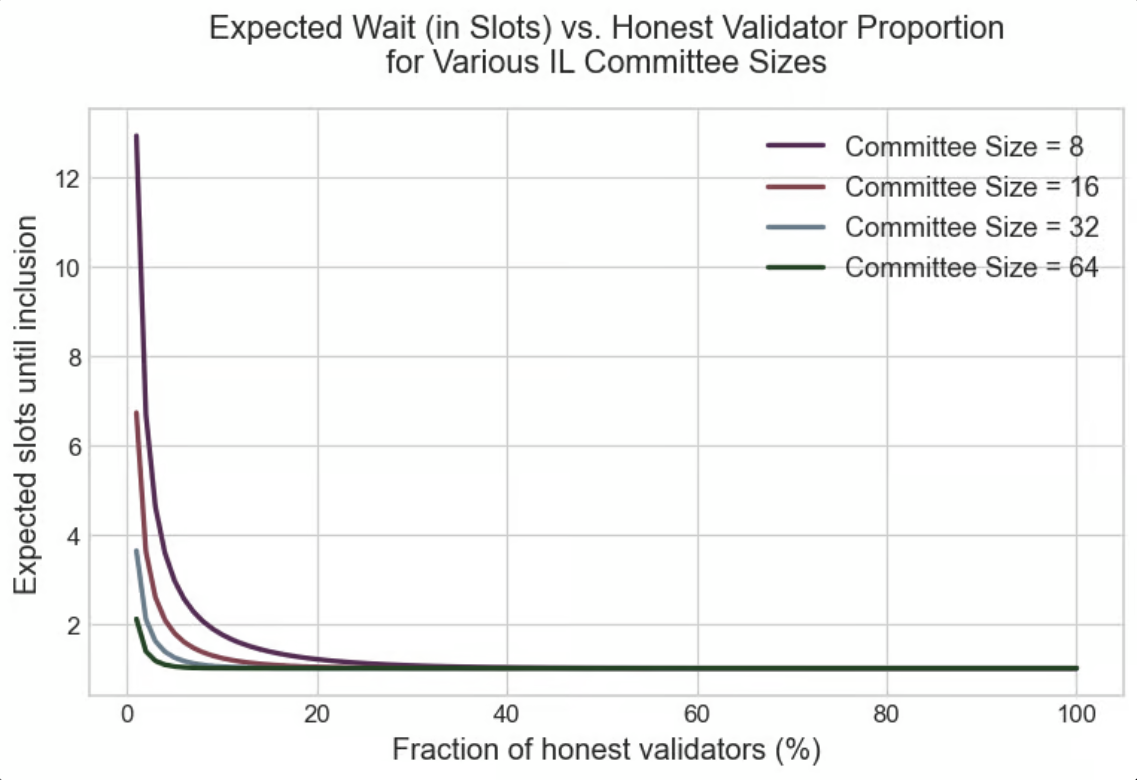
\includegraphics[width=0.5\textwidth]{focil effectiveness.PNG}
   \caption*{\textit{The IL Committee size \href{https://warpcast.com/soispoke/0xb2817f20}{doesn't have to be that big} to ensure censorship resistance}}
\end{wrapfigure}

An IL would be a list of transactions constructed by a committee of randomly selected attesters that each submit a list of transactions from the their own view of the public mempool. These lists would then be aggregated together (repeated transactions eliminated), and then submitted to the builder for inclusion. The block produced by the builder then gets checked by all attesters against this aggregated list by the committee of attesters. If the block resembles the IL above some canonically defined threshold, the block is considered valid. If the block does not resemble the IL enough, the block is not considered valid by the committee of attesters and it does not get included. The builder will have done the work but will miss out on their reward!

As long as one of the IL committee participants is honest, block builders can be held accountable; this is a 1-of-N honesty assumption. According to soispoke, for an IL committee of size 16, statistically only about 15\% of the validator set need to be honest for transactions to be included within the same slot. In this simulation, FOCIL seems to be a fairly robust mechanism for ensuring censorship resistance. 

One additional problem we have to solve is this - if we already sold block construction rights to block builders, how do we ensure a list of transactions from the public mempool are still included? The solution would be to allow builders flexibility around how the block is constructed, and as long as it is \textit{close enough} to the aggregated IL, the block is valid. What would likely happen, is the most valuable transactions would dominate the earliest part of the block to allow for close to optimum MEV extraction, and the later transactions in the block would more closely reflect the inclusion list. 

\subsubsubsection{Putting It All Together - Achieving all three properties}

In a post on ETHresear.ch, \href{https://x.com/mikeneuder}{Mike Neuder} discusses an approach that explicitly aims to achieve all three properties; he calls it \href{https://ethresear.ch/t/mechan-stein-alt-franken-ism/20321}{``Mechan-stein"}. Mike aims to combine the below sub-mechanisms into one approach by treating them as building blocks. 

\begin{aside}
    A brief aside - a ``slot" refers to the 12 second length of time where a block could be proposed, regardless if a block is proposed or not. The ``execution payload" refers to the transactions, or the contents of the block, the would occupy the block. The execution payload is what gets built by block builders and passed along to proposers for inclusion. 
\end{aside}

\begin{itemize}
    \item \textbf{Attesters sell their block building rights:} To achieve properties 1 \& 2, in this construction, attesters sell their block building right to builders, just as before in MEV-Boost, but this relationship is now formalized in protocol. The question becomes, \textit{when} to sell the rights - some set amount of time \textit{before} the slot has started, say for example, 32 slots before hand, or \textit{right at} the beginning of the slot? Mike debates the merits of both approaches; ultimately, one would have to be chosen over the other. \href{https://x.com/0xquintus?lang=en}{Quintus} from Flashbots also does a great job highlighting the tradeoff space around how to isolate the attester set \href{https://collective.flashbots.net/t/isolating-attesters-from-mev/3837}{here}. 
    \begin{itemize}
        \item \href{https://ethresear.ch/t/payload-timeliness-committee-ptc-an-epbs-design/16054}{\textit{Payload Timeliness Committee}} \textbf{\textit{(PTC)}} involves attesters auctioning off their block building rights \textit{during the slot}, encouraging builder competition. Potential draw-back here being that because of the ``real time" nature of the auction, this \textit{may} encourage sophisticated strategies by the attesters during the auction process to maximize rewards. If only some of the attesters are sophisticated enough to employ these tactics, it which might jeopardize property \#2, ensuring attester duties remain as \textit{unsophisticated} as possible. \textbf{PTC} effectively enshrines the out-of-protocol block building market that MEV-Boost had established.  The name comes from a specific part of this mechanism that aims to hold block builders accountable, ensuring that the execution payload was delivered to the proposer on time, as opposed to delaying delivery in an attempt by the builder to maximize MEV extraction at the expense of network liveness. 
        \item \href{https://ethresear.ch/t/execution-auctions-as-an-alternative-to-execution-tickets/19894}{\textit{Execution Auctions}} \textit{(\textbf{EA)}} aim to enshrine a similar out-of-protocol block building market just as PTC, with the difference being that the auction occurs 32 slots ahead of the start of the slot. The main difference between running the auction during the slot versus running it ahead of time is that the block builders who are the best at \textit{predicting} the expectation value of MEV extraction from execution payloads would win out; this is likely quite a difficult endeavor and the most sophisticated block builders would have an inherent advantage. So \textbf{EA} could potentially achieve property \#2 more effectively than \textbf{PTC}, but not necessarily encourage as competitive of a builder market, property \#1.\footnote{Another concept takes this a step further. Instead of running the auction a mere 32 slots ahead of time, it creates the concept of \href{https://ethresear.ch/t/execution-tickets/17944}{``Execution Tickets"}, which would represent the right to  build at some random point in time in the future. \href{https://www.youtube.com/watch?v=IrJz4GZW-VM}{Link to a talk} Justin Drake gave at Columbia, and a great \href{https://www.ephema.io/blog/beyond-the-stars-an-introduction-to-execution-tickets-on-ethereum}{article} by \href{https://x.com/ephemalabs}{Ephema Labs.}} \href{https://x.com/malleshpai}{Malesh Pai} from Rice University and \href{https://x.com/MaxResnick1}{Max Resnick} point out \href{https://youtu.be/jhzf1Jj_vwI?si=IkrAPRJgqjeOfnEj}{in this talk} that there are some extreme risks of centralization in the block builder market by selling block building rights into the future, as opposed to a just-in-time auction like in PTC. 
    \end{itemize}
    \item \textbf{A transaction inclusion mechanism} is implemented to ensure censorship resistance for the protocol (by preventing transaction exclusion). \textbf{FOCIL} aims to meet that need, which is property \#3. With the builder having discretion over how the block is built as long as it meets the aggregated IL threshold, it's likely the highest value transactions would dominate the beginning of the block, with the latter portion of the block's contents resembling the IL more closely. 
\end{itemize}

The combination of the above two building blocks would together aim to achieve our three properties, and would look something like this (with \textbf{PTC} implemented instead of EA): 

\begin{figure}[H]
    \centering
    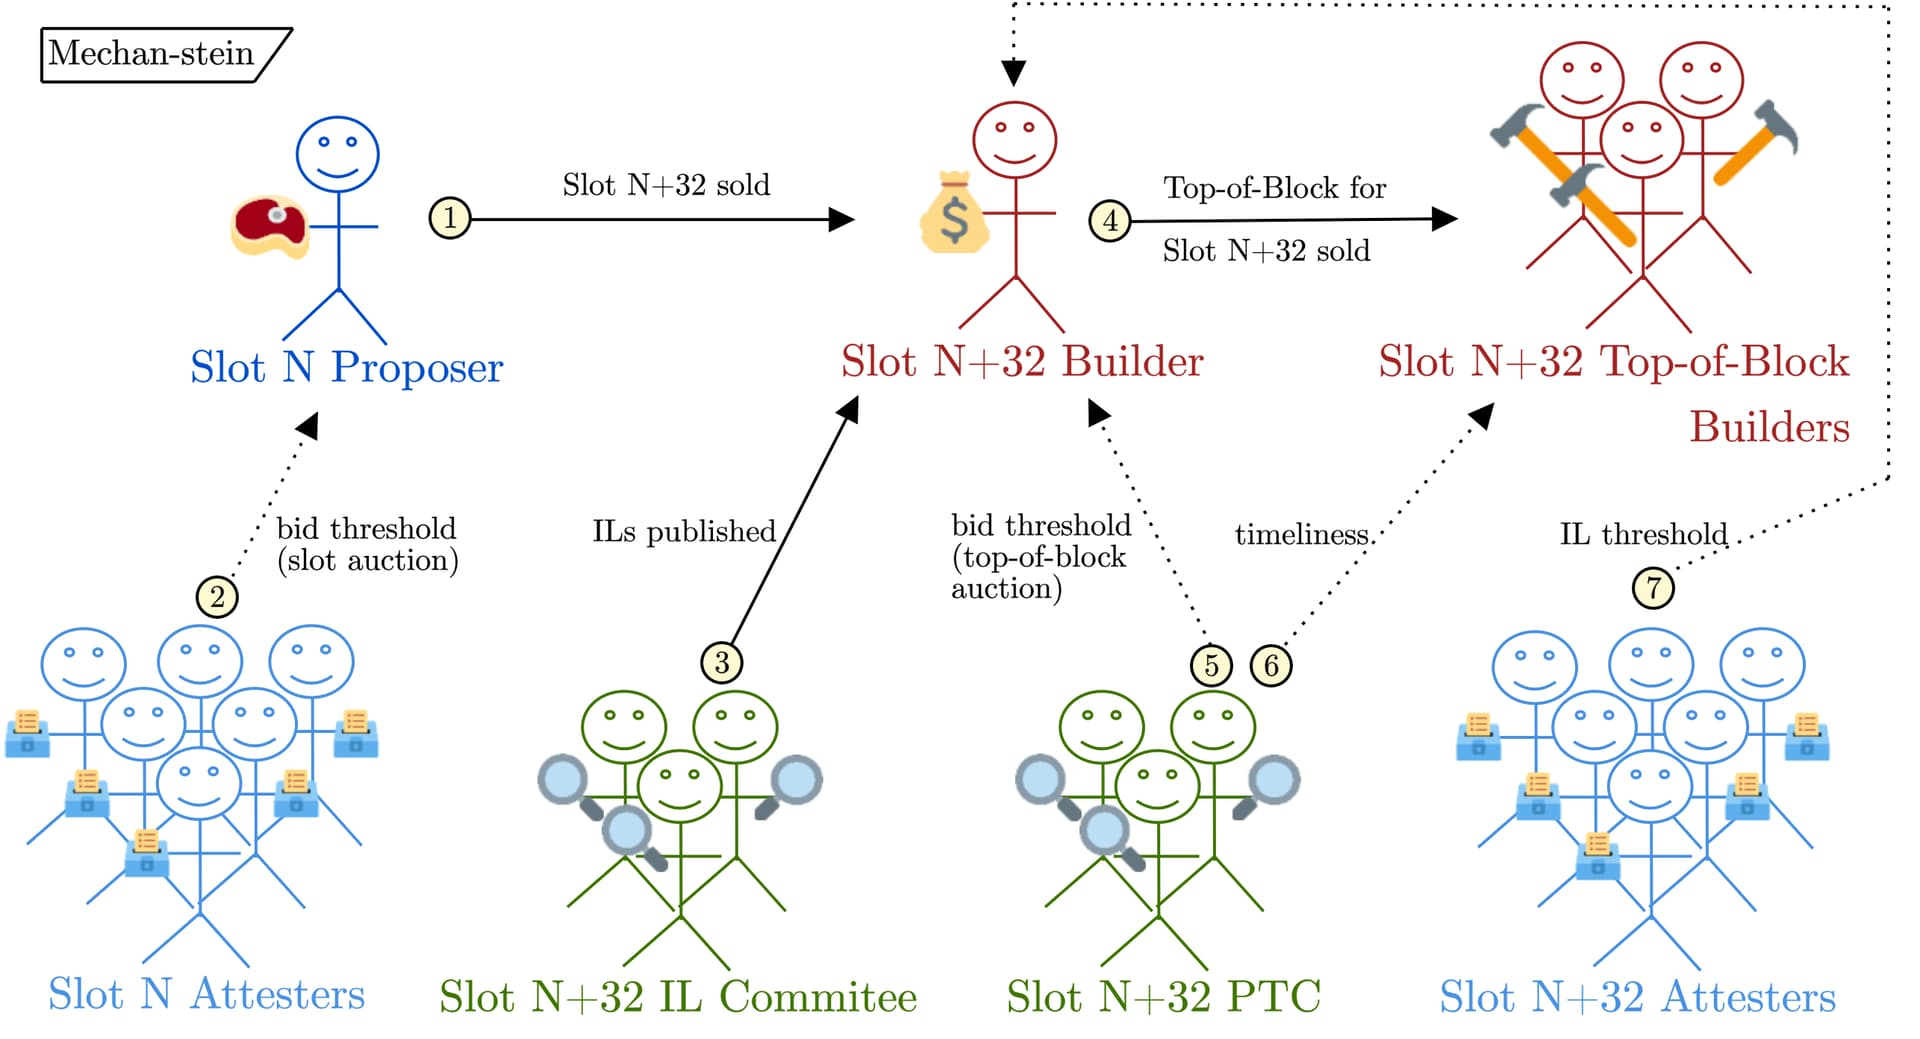
\includegraphics[width=0.85\linewidth]{mechanstein.jpeg}
    \caption{\textit{A lot going on here, which is one of the drawbacks of ``Mechan-stein" that Mike highlights in his article}}
\end{figure}

With Mechan-stein, we may have a relatively centralized builder market, but we would have one that is unable to censor, attestation remains a light task and block validation stays decentralized, and users cannot be excluded from participating in Ethereum. 

\begin{aside}
    \item \textbf{Honorable Mention: Multiple Concurrent Proposers} Another approach to mitigating MEV was introduced in \href{https://www.youtube.com/watch?v=mJLERWmQ2uw}{this talk} by \href{https://x.com/MaxResnick1}{Max Resnick.} Calling it BRAID, Max describes the implications of having more than one block proposer at the same time. This maximizes block producer competition and at the same time increases the cost of censoring transactions; the cost of censorship \href{https://ethresear.ch/t/concurrent-block-proposers-in-ethereum/18777}{scales linearly} with both the transaction tip (which would supplant the tip from the transaction that would otherwise have been included) and the number of proposers, since the attacker would have to censor all potential proposers. This approach would aim to achieve properties 1 \& 3, with property 2 being the tradeoff as it may require slightly higher proposer/attester hardware requirements. I leave this as an aside as Max has left the community and I am not sure who (or if) someone has picked up the torch in this research direction, although I would like to see it continue to be explored. 
\end{aside}

\subsubsubsection{Combatting Centralization in the Block Building Market}

Although centralization of the block building market is \href{https://vitalik.eth.limo/general/2021/12/06/endgame.html}{not as much of a threat to Ethereum as centralization at the attester layer}, it is still important; Flashbots is attempting to make the block building market more competitive with a piece of software called \href{https://collective.flashbots.net/t/introducing-buildernet/4173}{BuilderNet.} BuilderNet is a decentralized (although it has a white-list at the moment), open source, collaborative block building network. Galaxy research had a \href{https://youtu.be/3Ybrk7_Uyj0?si=p4T5TEKhSdC-kOEr}{great interview} with Robert Miller from Flashbots, the same Robert Miller who wrote the series on the Dark Forest of MEV. 

In today's MEV pipeline, block builders have built up trusted relationships with searchers who specialize in finding MEV opportunities onchain. These searchers send these opportunities, called orderflow, to the block builders they have built up these trusted relationships with. Searchers have to trust that block builders won't take these opportunities for themselves. The challenge with this is that these relationships are very unique to a small number of searchers and block builders; they're opaque and difficult for newcomers to compete with. 

\begin{wrapfigure}{r}{0.5\textwidth}
   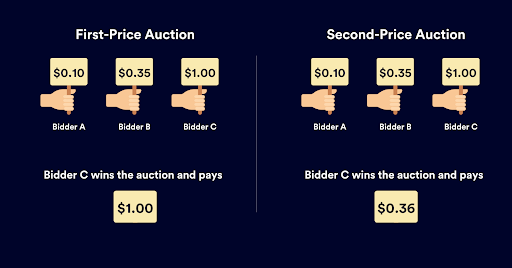
\includegraphics[width=0.5\textwidth]{second price.png}
   \caption*{\textit{First versus Second Price Auctions}}
\end{wrapfigure}

Remember, Flashbots' goal is to democratize these revenue streams by making them \textit{more transparent} to enable \textit{more competition.} BuilderNet's goal is to make these relationships obsolete by creating a network for builders to share orderflow from users, making orderflow a commodity. The question becomes, why would a successful block builder join BuilderNet, if they already enjoy exclusive orderflow from the searchers they have built relationships with? \clearpage

The reason is because BuilderNet will \textit{attract orderflow from users}, increasing MEV opportunities for block builders, by issuing \href{https://buildernet.org/docs/refunds}{\textit{user refunds}}, enabled by a mechanism inspired by \href{https://www.youtube.com/watch?v=VUN-k_nfDts}{\textit{second price auctions}}. BuilderNet bids in the MEV-Boost auction less than the true value of the block, then refunds users proportional to the value they contributed to the block from their orderflow. Through this refund mechanism, BuilderNet will be the best place for users to go who want to land a transaction onchain. This refund mechanism will attract infrastructure providers (who want to attract users), allowing BuilderNet to create a network effect around attracting the most valuable orderflow. which will also attract block builders who want a piece of the orderflow. 

As of now there are only 3 builders on BuilderNet, but Flashbots believes more builders will come as BuilderNet's network effect grows due to its superior access to user orderflow. BuilderNet has \href{https://buildernet.org/blog/beaverbuild}{attracted Beaver Build} to build blocks on BuilderNet, one of the most successful block builders on Ethereum. 

\subsubsection{The ETH Issuance Problem}

One challenge Ethereum faces is issuance of new Ether. There are a few reasons why this is a challenge, although at first glance it may not look like a problem: 

\begin{figure}[H]
    \centering
    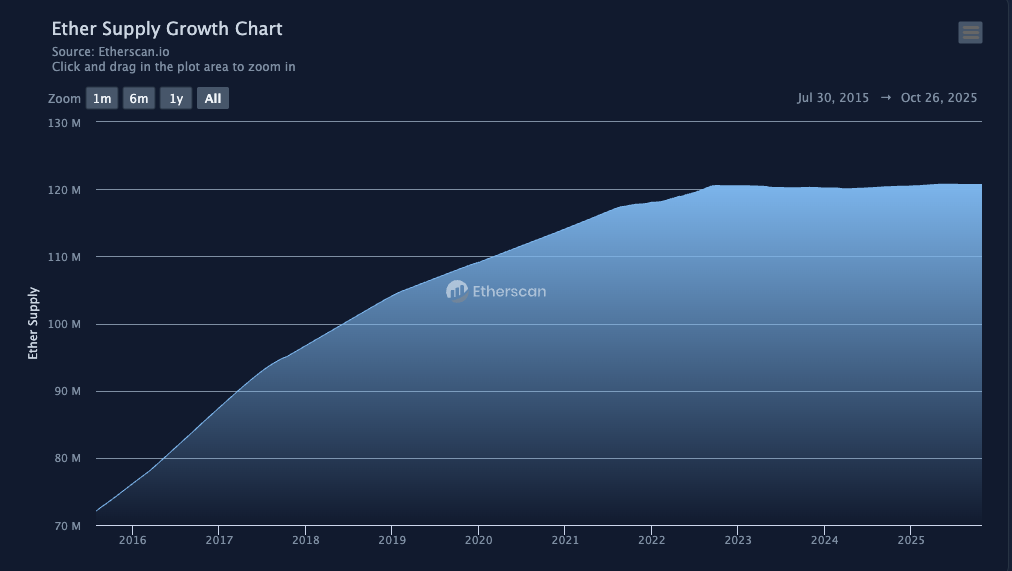
\includegraphics[width=0.95\linewidth]{ETH supply.png}
    \caption{\textit{How the total ETH supply has evolved over the years, from \href{https://etherscan.io/chart/ethersupplygrowth}{Etherscan}}}
\end{figure}

It should immediately be obvious that issuance of new ETH \textit{significantly} dropped almost overnight in September of 2022 with the activation of the Merge. The Ethereum network now \textit{inflates less per year than Bitcoin}, at least until the next Bitcoin halving in April 2028. 

Let's first briefly go over how issuance in Ethereum works. Validators are paid in ETH for securing the network; they have a few differing revenue streams. They earn ETH from attesting timeliness, \href{https://eth2book.info/capella/part2/incentives/rewards/#sync-committee-rewards}{sync committees} in support of \href{https://ethereum.org/developers/docs/nodes-and-clients/light-clients/}{light clients}, and for proposing blocks. They also earn revenue from MEV extracted from their block proposals, but this is not newly issued ETH, like the other sources of revenue are. 

Ethereum incentivizes validators to perform their duties well by paying them in ETH, but also by slashing their staked deposit in the case of misbehavior. As more ETH is staked, each individual validator earns a lower annual percentage yield, but the total network issuance of new ETH increases. The relationship between a validator's expected APR and the total ETH staked on the network is an \href{https://notes.ethereum.org/@mikeneuder/subsol#1-Inverse-Root-Curve-current-issuance}{inverse square root curve}: 

\begin{align}
    APR \approx \frac{2.6*64}{\sqrt{total\ staked\ ETH}}
\end{align}

An important concept is \textit{real yield}, which is the difference between the total issuance of the network and the expected yield for each validator. As an example, if each validator earned 2\% staking yield but the total network issuance was 2\% per year, then the \textit{real yield would be zero.}

\href{https://x.com/casparschwa}{Caspar} does a good job illustrating this concept with the following graphic from his \href{https://ethresear.ch/t/endgame-staking-economics-a-case-for-targeting/18751}{ethresear.ch post}: 

\begin{figure}[H]
    \centering
    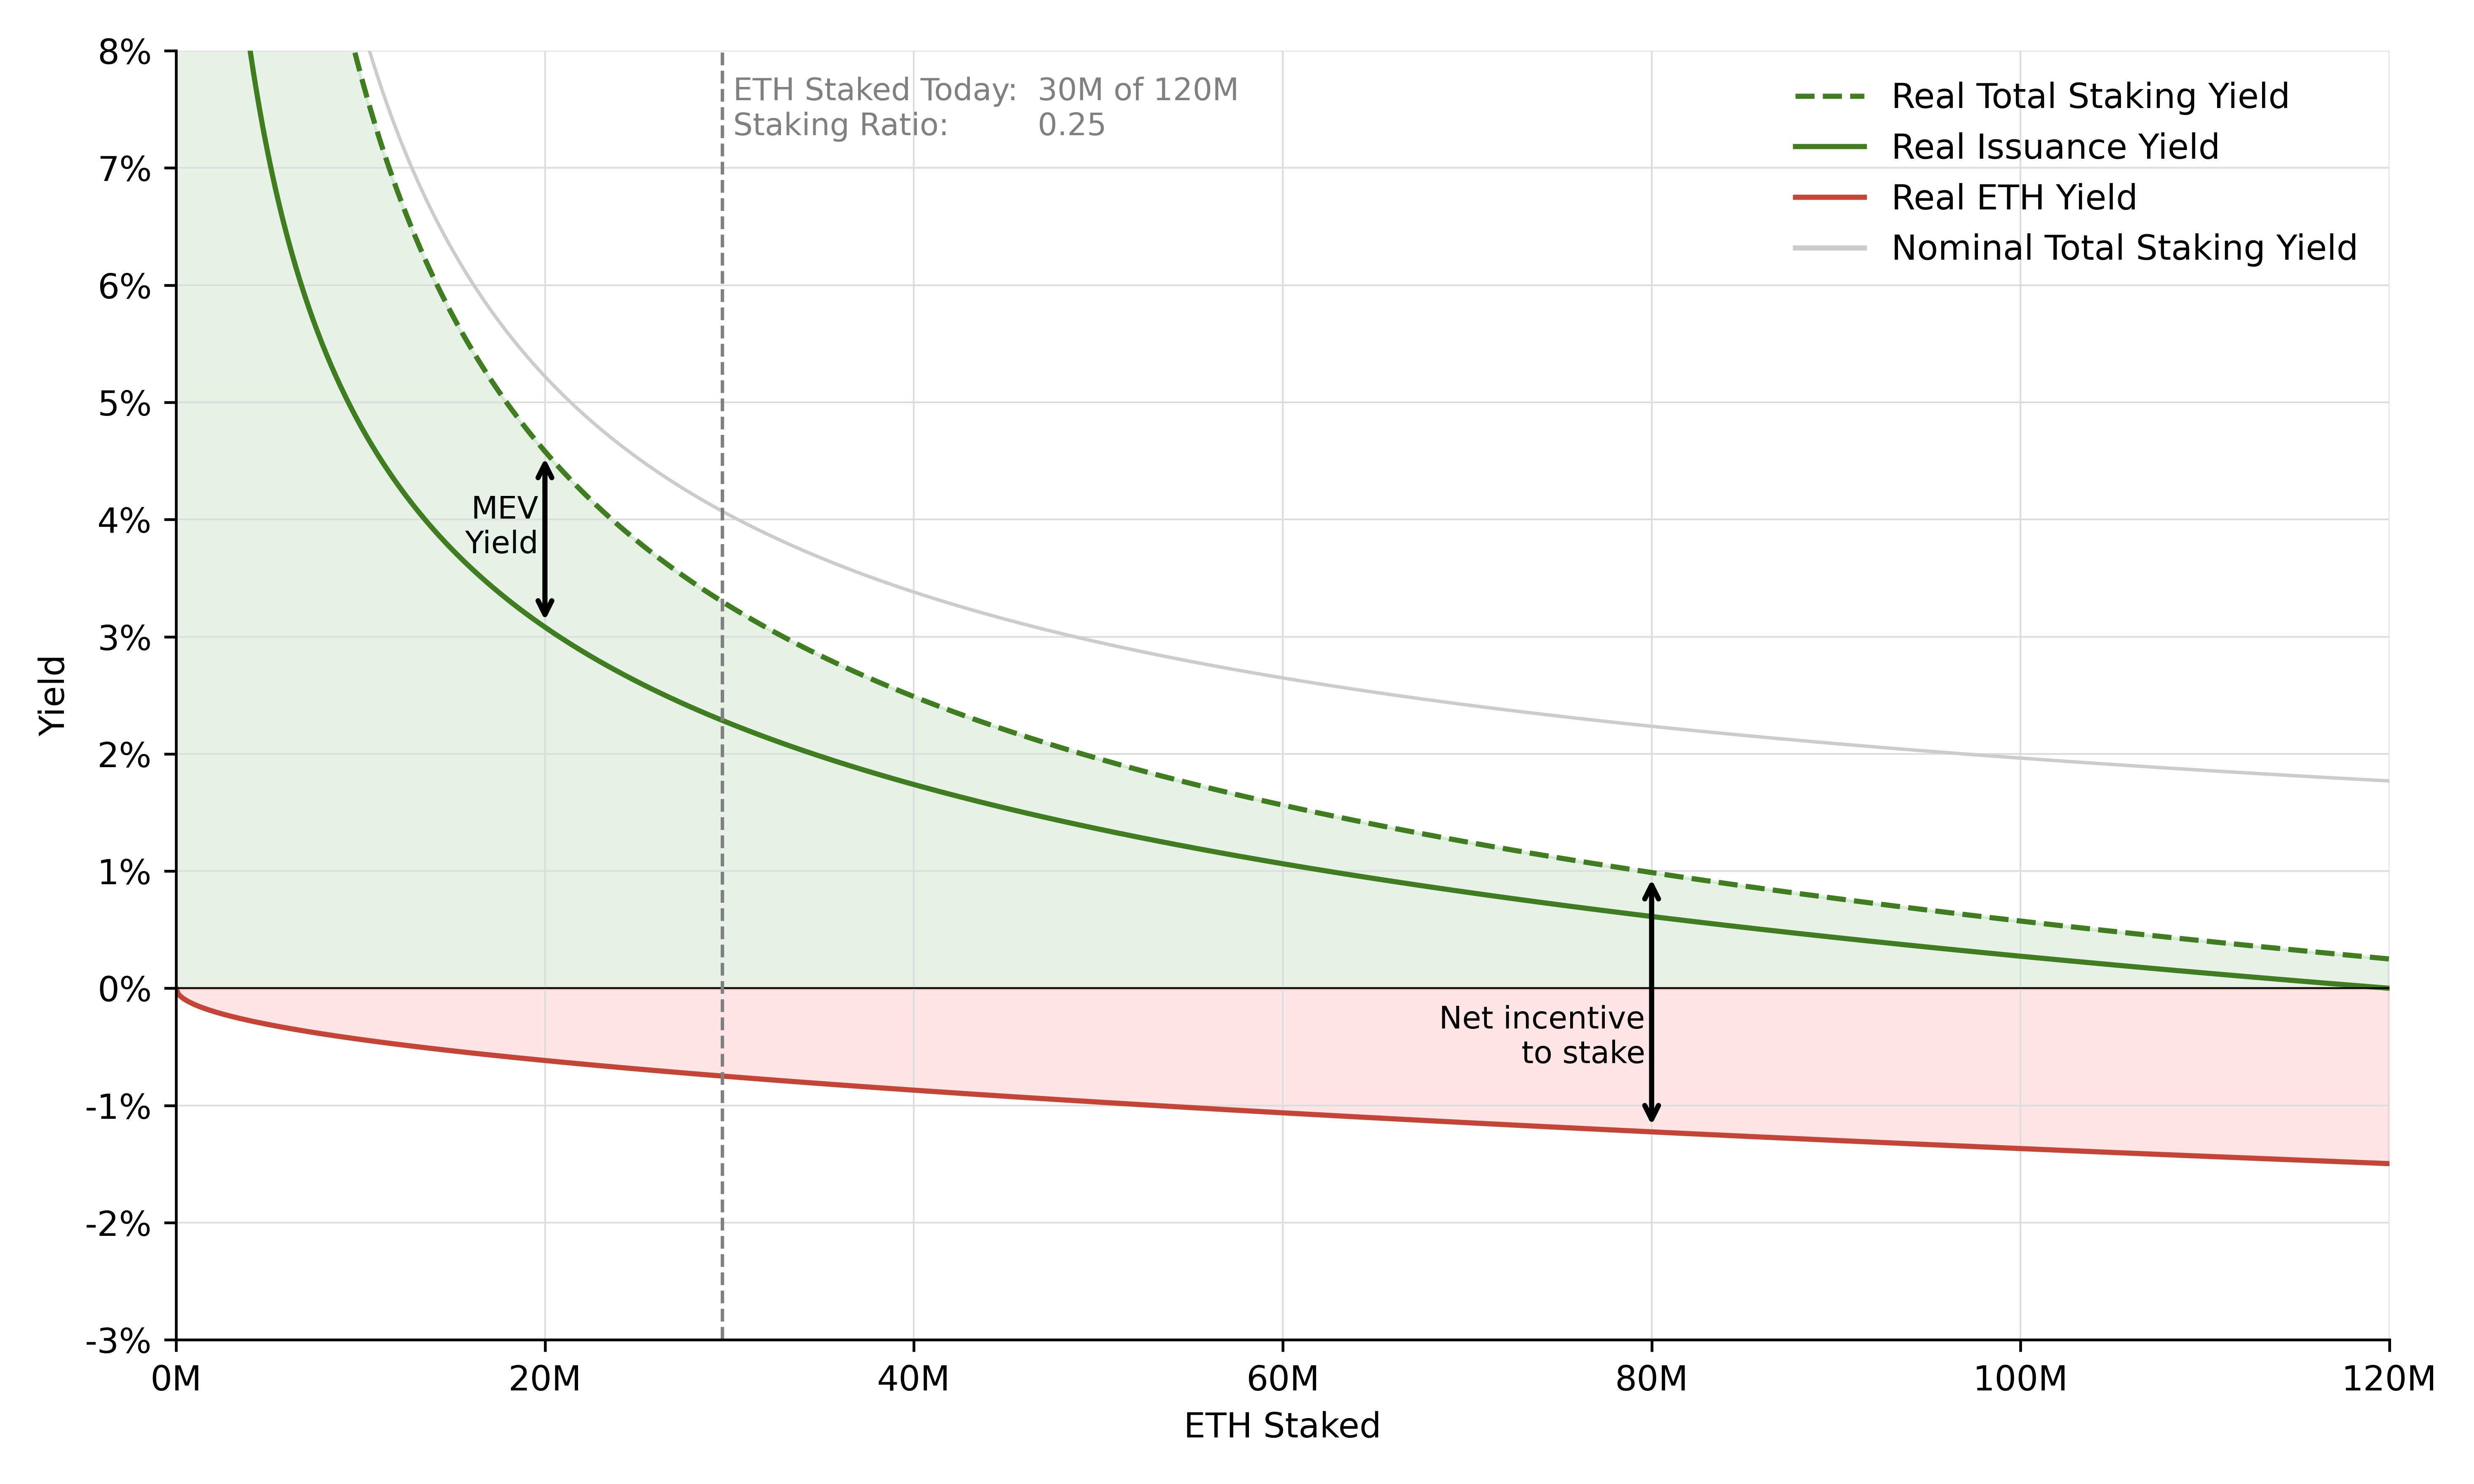
\includegraphics[width=0.95\linewidth]{real yield.png}
    \caption{\textit{As more ETH is staked, real yield (dashed green line) tends to near zero, even though nominal yield (gray line) remains close to 2\%}}
\end{figure}

Check out Ben Edgington's blog for a deep dive on how Ethereum's \href{https://eth2book.info/capella/part2/incentives/issuance/}{issuance} works and how \href{https://eth2book.info/capella/part2/incentives/rewards/}{rewards} for validators works. 

What exactly is the problem here? The problem comes down to the below elements: 

\subparagraph{Dilution Causes a Tragedy of the Commons} With staked ETH ETFs \href{https://x.com/Grayscale/status/1975147923387363421}{coming online}, staking ETH is about to become even more frictionless. \href{https://x.com/JustDeauIt}{Mike Nadeau} wrote an \href{https://thedefireport.io/research/the-50-billion-cascade#impact-on-economic-security}{excellent article} discussing the impacts of staked ETH ETFs. Liquid Staking Tokens and staked ETH ETFs allow holders to passively earn the staking yield. As staking friction falls, more ETH is staked, increasing the dilution for non-stakers; this creates a stronger incentive for them to stake just to avoid dilution. In a scenario where almost all ETH is staked due to this dynamic, ETH the asset would be suffering from 2\% dilution while stakers experience negative real yield, after accounting for taxes. 

\subparagraph{Loss of ETH as Permissionless Money:} As more Liquid Staking Tokens (LST) are minted, an LST could potentially gain strong network effects around having more liquidity than un-staked ETH. This introduces systemic risk to the ecosystem, one that would not exist if ETH remains the dominant form of permissionless collateral in the ecosystem. \\

\href{https://x.com/weboftrees}{Anders} did a good job \href{https://youtu.be/m91Wu6-cdwk?si=pEZ6Y7L0K3Wq7ZQa}{at Devcon} in November of 2024 discussing his ``\href{https://ethresear.ch/t/practical-endgame-on-issuance-policy/20747}{Practical Endgame for Issuance Policy}" and I am in favor of this approach. 

\subsubsection{Making Ethereum Quantum Resistant}
\label{Making Ethereum Quantum Resistant}

Ethereum is working towards hardening itself against quantum threats, but it is very early in exploring this research path, \textit{so this section will generalize and be very brief.} Probably the best resource to deep dive this topic is this inaugural \href{https://www.youtube.com/watch?v=g-PDKIAqw-A&list=PLJqWcTqh_zKGPctGzVOBllZnCPQj-g7d3}{post-quantum workshop}, a 3 day workshop specifically on Ethereum's quantum resistance roadmap that was just posted four days ago (as of writing). 

Quantum resistant cryptography \href{https://en.wikipedia.org/wiki/Post-quantum_cryptography}{already exists} as a cryptographic primitive, but the challenge for Ethereum will again come back to the limitations of the speed of signature aggregation, just as in the section on \hyperref[Single Slot Finality]{Single Slot Finality.} Quantum-resistant signatures, were Ethereum to switch to them today, would introduce a 10x performance degradation to Ethereum's TPS. \href{https://youtu.be/g-PDKIAqw-A?si=uYvITr67sQnTHISe&t=887}{According to Justin Drake}, ``\textit{this is one of the last things we need to do to de-risk this direction}" (quantum resistance, my emphasis). 

The most important takeaway here is that \textit{Ethereum is taking Quantum Computing very seriously and is planning for this eventuality.} 

\clearpage

\section{Endgame}

Ethereum boasts \href{https://ethereumuptime.org/}{100\% uptime} and will become the global censorship resistant, neutral public infrastructure that powers global finance. 

\hyperref[Single Slot Finality]{\textbf{Single Slot Finality}} will enable sub $\approx$ 30 second economic finality, \hyperref[Single Secret Leader Election]{\textbf{secret leader election}} will make Ethereum highly DDoS resistant, and \hyperref[Preconfirmations]{\textbf{preconfirmations}} will provide users with a fast, fintech-like experience. 

\hyperref[PeerDAS]{Data Availability Sampling} will allow the network to load-share Layer 2 transaction data across the network, allowing scalability and decentralization to increase \textit{in tandem.}

\hyperref[Validity Proofs]{\textbf{Validity Proofs}} and \hyperref[Stateless Verification]{\textbf{stateless verification}} will allow attesting to happen on very compute limited devices, even smart watches, while allowing the gas limit to increase 100 fold, to allow as much as 10k TPS on Ethereum layer 1. Validity proofs will also unlock \hyperref[Native Rollups]{Native Rollups}, making rollups trustless and decreasing their development timelines.

Ethereum is expending serious effort towards \hyperref[Making Ethereum Quantum Resistant]{post-quantum security}. 

All while Ethereum is the most incentive compatible public infrastructure for all participants, with an attester set that is more isolated from centralizing forces than on any other blockchain. 

The result is that Ethereum's network effects are growing stronger by the day, and name brands are \href{https://ethereumadoption.com/built-on-ethereum?view=byDate}{building on Ethereum}. 

The financial infrastructure of the world will be built on Ethereum. 

\section{Resources}

\subsection{Data Dashboards}

\begin{itemize}
    \item \href{https://ethereumadoption.com/built-on-ethereum/}{Ethereum Adoption} - a dashboard that showcases house hold brands building on Ethereum, built by \href{https://x.com/hanni_abu}{Hanniabu}
    \item \href{https://www.validatorqueue.com/}{Staking Entry and Exit Queue Dashboard} - dashboard for staking entry and exit queue, also built by \href{https://x.com/hanni_abu}{Hanniabu}
    \item \href{https://www.growthepie.com/}{Grow the Pie} - A great data source for all things Ethereum
    \item \href{https://defillama.com/}{DeFiLlama} - Another great data source for all things crypto related
    \item \href{https://l2beat.com/scaling/summary}{L2Beat} - focused on Ethereum Layer 2s, also a great educational resource
    \item \href{https://www.strategicethreserve.xyz/}{Strategic ETH Reserve} - A data source for all things Ethereum Treasuries and Ethereum ETFs related
    \item \href{https://ultrasound.money/?timeFrame=since_merge}{Ultrasound.money} - A website focused on Ethereum's supply
    \item \href{https://dotpics.info/}{Toni's Collection of Dashboards} - A collection of dashboards built by \href{https://x.com/nero_eth}{Toni} from the Ethereum Foundation which features stats on censorship, block reorgs, MEV-Boost, and more
    \item \href{https://dune.com/discover/content/trending}{Dune Analytics} - the best source of real time blockchain data
    \item \href{https://forkcast.org/}{Forkcast} - An informational website about Ethereum's upcoming hardforks
    \item \href{https://ethproofs.org/}{ETH Proofs.org} - A website dedicated to displaying zkVM block proving times and trust assumptions associated with zkVMs
    \item \href{https://dashboard.etherealize.com/}{Etherealize's dashboard} - a beautiful dashboard focused on ETH being a store of value, built by \href{https://x.com/Etherealize_io}{Etherealize}
    \item \href{https://orderflow.art/}{Orderflow.art}, an interactive dashboard showing the lifecycle of transactions on Ethereum
    \item \href{https://app.rwa.xyz/}{RWA.xyz} - a beautiful dashboard tracking Real-World Assets hosted on the largest blockchains
    \item \href{https://www.ethismoney.xyz/}{ETH is Money} - an ETH is money dashboard
    \item \href{https://leanroadmap.org/}{Lean Consensus R\&D Roadmap} - A roadmap dashboard focused on Ethereum's Consensus layer
    \item \href{https://ethroadmap.com/}{ETH Roadmap} - focused on Ethereum's roadmap as outlined by Vitalik's six research tracks, although now outdated
    \item \href{https://rollup.wtf/}{Rollup.wtf} A real time dashboard that displays TPS for the constellation of L2s
    
\subsection{Podcasts and Youtube Channels}
    \item Justin Drake's \href{https://youtu.be/8mJDt8TGebc?si=pu-F31lkjmbDXMcA}{thoughts} on the Ethereum Roadmap at the Bankless Summit last year
    \item Three more Justin Drake interviews: \href{https://youtu.be/0q-qT67yyVs?si=gOJnrS50vgXIHTEv}{1}, \quad \href{https://youtu.be/jUFVOUq0-fc?si=Q0UiEPqx4iAnnTSS}{2}, \quad \href{https://youtu.be/88FDeg5JaUk?si=VWmv2tByzgNVo0oZ}{3}
    \item \href{https://www.youtube.com/@Bankless}{The Bankless Podcast} - An Ethereum focused podcast by \href{https://x.com/TrustlessState}{David Hoffman} and \href{https://x.com/RyanSAdams}{Ryan Sean Adams}
    \item \href{https://www.youtube.com/@TheDailyGwei}{The Daily Gwei Podcast} - one of the best sources of Ethereum news by \href{https://x.com/sassal0x}{Anthony Sassano}
    \item \href{https://www.youtube.com/@EthereumProtocol}{Ethereum's More Active Youtube Channel} and another \href{https://www.youtube.com/@EthereumFoundation}{older channel}
    \item \href{https://www.youtube.com/watch?v=KNJGPI0fuFA&list=PLEGCF-WLh2RLOHv_xUGLqRts_9JxrckiA}{Tim Roughgarden's} youtube lecture series on blockchains

\subsection{Technical Resources and Reading Materials}
    \item An Ethereum \href{https://ethereum.org/glossary/#proof-of-stake}{Glossary}
    \item A 6 part \href{https://vitalik.eth.limo/general/2024/10/14/futures1.html}{blog} series by Vitalik that deep dives Ethereum's roadmap
    \item \href{https://ethresear.ch/}{ETH Research} - Ethereum's premier research forum
    \item \href{https://ethereum-magicians.org/}{ETH Magicians} - A less formal forum for discussing Ethereum's upcoming upgrades
    \item \href{https://eth2book.info/latest/}{Eth2Book} - Ben Edington's technical deep dive on Ethereum
    \item \href{https://epf.wiki/#/}{EPF Wiki} - ``a collection of technical resources about Ethereum", some really great stuff here
    \item \href{https://inevitableeth.com/}{Inevitable ETH .com} - Ethereum's wikipedia
    \item \href{https://ethereum.org/}{Ethereum.org} - An open source website that is an educational resource, funded by the Ethereum Foundation
    \item \href{https://vitalik.eth.limo/}{Vitalik's Website} - where he blogs about whatever he's interested in
    \item L2Beat's comprehensive resource on \href{https://native-rollups.l2beat.com/}{Native Rollups}
    \item \href{https://x.com/ib1gymnast/status/1475296136277606401}{My first paper}, an overview of the Ethereum ecosystem as a whole
    \item \href{https://eips.ethereum.org/}{Ethereum Improvement Proposals} - website dedicated to EIPs
    \item A \href{https://mirror.xyz/nixo.eth/TS-GwCEAKD_UTOE2_SCA_eFWyHstVAtGGn2Hu8mMezQ}{breakdown} of the structure of the R\&D teams at the Ethereum Foundation by \href{https://x.com/nixorokish}{nixo.eth}
    
\end{itemize}

\section{Donate}

If this paper brought you value, consider donating to one my 0xsplits contract addresses below. \\

All of the below splits contracts automatically split up funds on whichever network you choose to donate on according to the below: 

\begin{itemize}
    \item 49.5\% of donated funds go to the \href{https://x.com/ProtocolGuild}{Protocol Guild}
    \item 49.5\% of donated funds go to me
    \item 1\% of donated funds go to \href{https://x.com/0xSplits}{0xSplits} to help fund their team
\end{itemize}

The Protocol Guild is an independent funding organization that helps to fund the work of $\approx$ 190 open source Ethereum core developers. \\

The Splits contracts I made below are immutable, meaning they can never change, so you know exactly where your donated money will go and you can verify that onchain. You can verify The Protocol Guild's donation addresses \href{https://protocol-guild.readthedocs.io/en/latest/03-donate.html}{here}. \\

\begin{itemize}
    \item \textbf{Ethereum:} \href{https://app.splits.org/accounts/0xC7560fCBf74585d4440EbCfcA5B807b46d0B59A0/?chainId=1}{0xC7560fCBf74585d4440EbCfcA5B807b46d0B59A0}
    \item \textbf{Base Network:} \href{https://app.splits.org/accounts/0xca7Cb8F47B0e2Fd993Daa73d37e90A4E18502b30/?chainId=8453}{0xca7Cb8F47B0e2Fd993Daa73d37e90A4E18502b30}
    \item \textbf{Arbitrum:} \href{https://app.splits.org/accounts/0x7C64914Dd25e4bFC479D0ed9aB7A3046585c6c6f/?chainId=42161}{0x7C64914Dd25e4bFC479D0ed9aB7A3046585c6c6f}
    \item \textbf{Optimism's OP Mainnet:} \href{https://app.splits.org/accounts/0xcC2Fed4256C07e82fdbb4f3E3A413802A30F76Bb/?chainId=10}{0xcC2Fed4256C07e82fdbb4f3E3A413802A30F76Bb}
\end{itemize}

\end{document}